\documentclass{article}

\usepackage{amsmath}

\usepackage{graphicx}

\usepackage{hyperref}

\usepackage[utf8]{inputenc}

\usepackage{subcaption}

\usepackage{geometry}

\usepackage{multirow}

\usepackage{siunitx}

\usepackage[square,numbers]{natbib}

\usepackage[english]{babel}
%Includes "References" in the table of contents
\usepackage[nottoc]{tocbibind}

\usepackage[parfill]{parskip}

\usepackage[toc,page]{appendix}

\usepackage{tabularx}

\usepackage{booktabs}

\newcommand{\pvec}[1]{\vec{#1}\mkern2mu\vphantom{#1}}

\DeclareSIUnit{\angstrom}{\textup{\AA}}

\geometry{legalpaper, portrait, margin=1in}

\title{Lab Report}

\author{Jamal Ghaith}
\author{Anas Roumieh}

\date{01.04.2024}

\begin{document}

\begin{titlepage}
	\centering
	{\scshape\LARGE University of Leipzig \par}
	\vspace{1cm}
	{\scshape\ Advanced Labs\par}
	\vspace{1.5cm}
	{\huge\bfseries Lab report\par}
	\vspace{2cm}
	{\huge\bfseries X-Ray diffraction (XRD)\par}
	\vspace{2cm}
	{\Large Jamal Ghaith 3792970\par}
    {\Large Anas Roumieh 3766647\par}
	\vfill

    {\Large Conducted on: 23.04.2024 \par}
	\vfill
\end{titlepage}


\tableofcontents
\pagenumbering{gobble}
\pagebreak{}
\pagenumbering{arabic}

\section{Introduction}

\subsection{Generation of X-rays, Bremsstrahlung and characteristic spectrum}

X-rays are a form of electromagnetic radiation similar to light but with much shorter wavelengths. The standard unit for measuring X-ray wavelengths is the angstrom (Å), which is equivalent to $10^{-10}$ meters. In diffraction experiments, X-ray wavelengths typically range from about 0.5 to 2.5 Å \cite{bernarddeniscullity_2015_elements}. For comparison, visible light has a wavelength around 6000 Å. 

X-rays are generated when a charged particle with enough kinetic energy decelerates rapidly. Typically, electrons are used for this purpose, with the radiation being produced in an X-ray tube that contains an electron source and two metal electrodes. The voltage across these electrodes $U$, which is often tens of thousands of volts, swiftly pulls the electrons to the anode or target, where they collide with high velocity. At the point of impact, X-rays are produced and radiate in all directions. The electrons strike the anode and a small portion of their kinetic energy $eU$ is emitted in the form of X-rays (around 1\%), while the rest dissipates as heat. 

X-rays are generated due to two effects, which result in two different spectra, a continuous and a sharply peaked one:

\begin{enumerate}

\item \textit{Bremsstrahlung}

Results when charged particles (e.g. electrons) are rapidly decelerated. Note that not all electrons decelerate in the same fashion. Rather, some halt abruptly upon impact, instantly releasing all their energy, while others zigzag through the target's atoms, gradually losing portions of their kinetic energy until fully dissipated. Those electrons halted in a single collision emit photons with the highest energy, corresponding to x-rays with the shortest wavelength. These electrons transfer their entire energy into photon energy and define the maximum energy of the radiation that can be emitted which is equal to their kinetic energy. This defines a lower limit on the wavelength of the radiation \cite{bernarddeniscullity_2015_elements}: 
\begin{equation}
    \lambda \geq \lambda_{\min} = \frac{hc}{eU}
\end{equation}

\item \textit{Characteristic peaks}

The narrow peaks observed are a consequence of high-energy electrons from the cathode exciting electrons within the anode material. This excitation causes electrons from inner shells to occupy higher energy levels, leaving vacancies behind them. Subsequently, electrons from outer shells fill these vacancies, emitting energy in the form of X-ray radiation with specific wavelengths corresponding to particular transitions. Each peak, or "line," signifies a transition between different orbitals.
\begin{figure}[h]
    \centering
    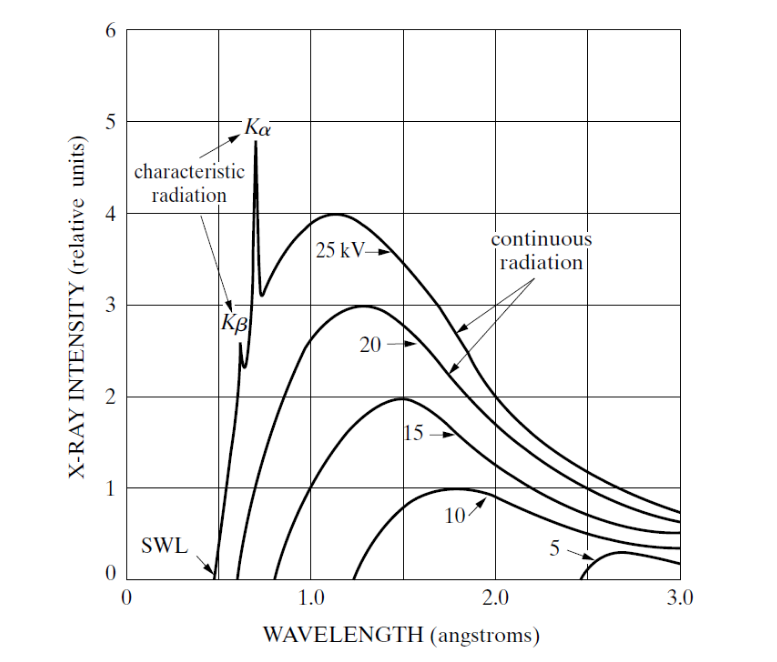
\includegraphics[width=0.8\textwidth]{Figures/fig1.png}
    \caption{X-ray emission spectra of Tungsten for different voltages. Notice that the characteristic peaks only show up after a voltage threshold}
    \label{fig:xrayemission}
\end{figure}
\end{enumerate}

\pagebreak{}

\subsection{Nomenclature of designation of characteristic X-ray lines}
Characteristic X-ray lines are uniquely labeled according to the metal used for their production. They are sorted into categories labeled as K, L, M, and so forth, arranged by increasing wavelength (or decreasing energy). Each letter corresponds to a principal quantum number, starting with n = 1, then n = 2,3,4 and so on. The K lines are the ones typically useful in X-ray diffraction experiments, since the lines corresponding to longer wavelengths are easily absorbed. The K set is comprised of many lines due to vacancies being filled by electrons from the L shell (K$\alpha$) or the M shell (K$\beta$). However, we are only concerned with the three strongest ones for our purposes: K$\alpha_1$, K$\alpha_2$ and K$\beta$. 

\begin{figure}[h]
    \centering
    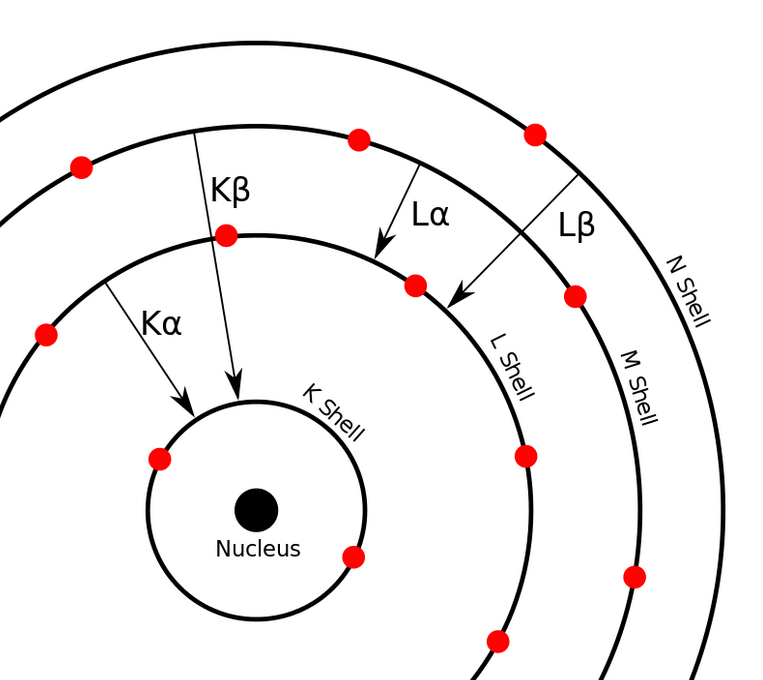
\includegraphics[width=0.5\textwidth]{Figures/Screenshot 2024-06-02 204357.png}
    \caption{Characteristic X-ray transitions [wiki photo]}
    \label{fig:characteristicxraytransitions}
\end{figure}

The reason behind the $\alpha_1$ and $\alpha_2$ components is fine structure (spin-orbit coupling). The two split components are referred to as a $doublet$. Their wavelengths are so close together such that they are not always observed and then we only talk about a K$\alpha$ line, a $singlet$. Note that it is easier for electrons to jump from an L shell to fill vacancies in the K shell. Hence, the K$\alpha$ lines are significantly stronger than the K$\beta$ lines (Fig.3). For any element, the $\alpha_1$ component is usually about twice as strong as the the $\alpha_2$ component \cite{bernarddeniscullity_2015_elements}. The K$\alpha_1$ line occurs due to the transition $2^2 P_{1 / 2} \rightarrow 1^2 S_{1 / 2}$, while the transition $2^2 P_{3 / 2} \rightarrow$ $1^2 S_{1 / 2}$ gives rise to the K$\alpha_2$ line. Recall the relevant  selection rules here: $\Delta l = \pm1$ and $\Delta j = 0,\pm1$. The $2^2 P_{3 / 2}$ state is statistically more populated by electrons than $2^2 P_{1 / 2}$ due to the two additional $m_j = \pm\frac{3}{2}$ states which causes the 2-to-1 ratio between $\alpha_1$ and $\alpha_2$. 

\begin{figure}[h]
    \centering
    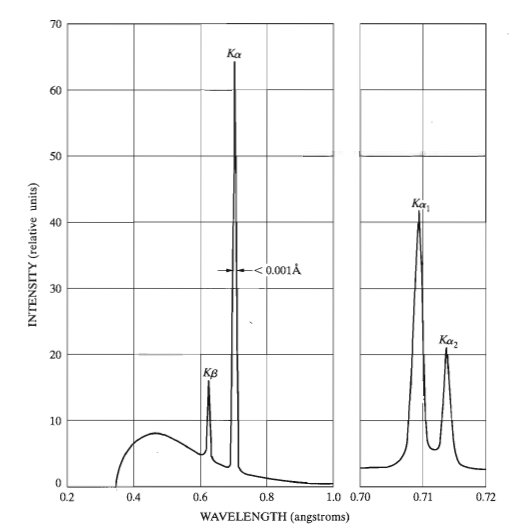
\includegraphics[width=0.5\linewidth]{Figures/image2.png}
    \caption{Spectrum of Molybdenum at 35 kV. Line widths not to scale. Resolved K$\alpha$ doublet is shown on an expanded wavelength scale at the right \cite{bernarddeniscullity_2015_elements}}
    \label{fig:mo35kv}
\end{figure}

This notation for spectral lines is referred to as Siegbahn notation, which is conventionally employed in X-ray spectroscopy and often preferred over more detailed notations like the term symbol notation.

\pagebreak{}

\subsection{Absorption of X-rays}
When x-rays interact with matter, they undergo both transmission and absorption. Röntgen's early findings revealed that the reduction in the intensity $I$ of an x-ray beam passing through a homogeneous substance is proportional to the distance covered $x$. Mathematically, this is described by the equation \cite{bernarddeniscullity_2015_elements}:

\begin{equation}
\label{eq:absorption}
    -\frac{dI}{I}= \mu dx
\end{equation}

the constant $\mu$ is the linear absorption coefficient and depends on the material, its density and the wavelength of the X-rays. Equation (2) can be solved by integration yielding: 
\begin{equation}
    I_x = I_0 e^{-(\mu/\rho)\rho x}
\end{equation}

The reason for inserting the density in the solution is that the quantity $\mu/\rho$, termed the \textit{mass absorption coefficient}, is the same regardless of the physical state of the material (gas, liquid or solid).

Analyzing the variation of the mass absorption coefficient provides information on how X-rays interact with atoms. The typical $\mu/\rho$ versus wavelength curve displays characteristic curves, known as branches, which are separated by sharp discontinuities (see Figure 6). This occurs because the primary cause of the reduction in the intensity of the incoming beam is true absorption, due to electronic transitions within the atoms of the substance, rather than scattering (random loss of intensity). Similarly to how an energetic incident electron can eject an inner-shell electron, an X-ray photon with sufficient energy can do the same

\begin{figure}[h]
    \centering
    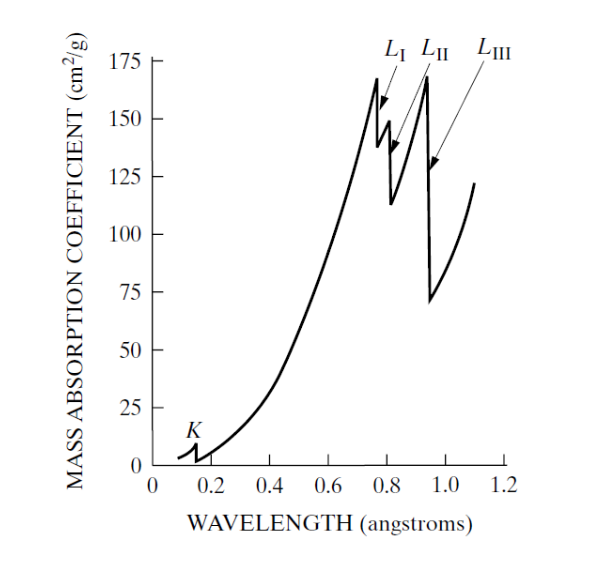
\includegraphics[width=0.5\linewidth]{Figures/image1.png}
    \caption{Absorption coefficient of lead, with K and L absorption edges \cite{bernarddeniscullity_2015_elements}}
    \label{fig:enter-label}
\end{figure}

The absorption profile displays not only the peaks corresponding to each critical energy value but also the small peaks of the fine structure of each level.
\\\\
Along each branch, the absorption coefficient varies with wavelength approximately following the relation \cite{bernarddeniscullity_2015_elements}:

\begin{equation}
    \mu/\rho = k\lambda^3 Z^3
\end{equation}
\\
Where $k$ is a constant with a different value for each branch of the curve, and $Z$ is the atomic number of the absorbent material. Consequently, short-wavelength X-rays are highly penetrating and are referred to as hard X-rays, while long-wavelength X-rays are easily absorbed and are known as soft X-rays. The shape of the graph in Figure 4 becomes clear when one considers that increasing frequency opens new absorption channels whenever a critical value is reached, corresponding to the minimum energy required to create a specific vacancy. Sometimes, instead of emitting the energy as an X-ray, the energy can be transferred to another electron, causing it to be ejected from the atom. This phenomenon is known as the Auger effect which happens mostly in lighter elements (Z$<$31).

\pagebreak{}

\subsection{Filtering of X-rays}
X-ray diffraction experiments typically require highly monochromatic radiation. However, as seen in Figure 5, the high voltage utilized in X-ray tubes causes emission of not only the intense K$\alpha$ line, but also the weaker K$\beta$ line and the continuous spectrum. Hence, the use of a \textit{filter} whose K absorption edge is between the K$\alpha$ and K$\beta$ wavelengths of the material. This will lead to the reduction of the intensity of the undesired lines relative to the K$\alpha$ line. 

\begin{figure}[h]
    \centering
    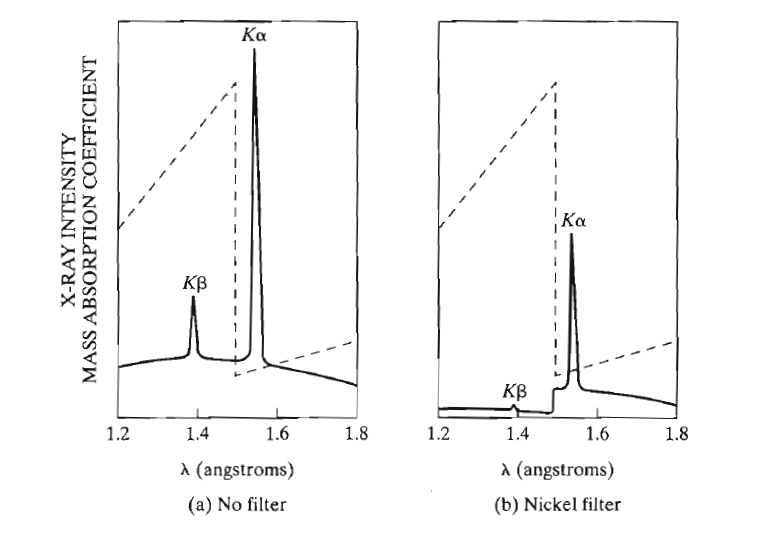
\includegraphics[width=0.5\linewidth]{Figures/image.png}
    \caption{Comparison of the spectra of copper radiation (a) before and (b) after passage through a nickel filter (schematic). The dashed line is the mass absorption coefficient of nickel. \cite{bernarddeniscullity_2015_elements}}
    \label{fig:enter-label}
\end{figure}

The filtration becomes better (i.e. the ratio of intensity of K$\beta$ to K$\alpha$ becomes lower) when the thickness of the filter increases. However, since the intensity of the K$\alpha$ line is affected, the process is not perfect. One must achieve a balance between a sufficient suppression of the K$\beta$ component and the inevitable weakening of the K$\alpha$ line. In practice, halving the original value of K$\alpha$ usually decreases the K$\beta$ to K$\alpha$ intensity ratio from 1/9 in the incident beam to around 1/500 in the transmitted beam, which is sufficiently low \cite{bernarddeniscullity_2015_elements}. 

\pagebreak{}

\subsection{Crystal systems and Miller indices}
\label{subsection:CrystalSystems}

An ideal crystal is formed by infinitely repeating identical groups of atoms, referred to as the basis. The mathematical points to which the basis is attached form the lattice. In three dimensions, the lattice can be defined by three translation vectors $\vec{a}_1$, $\vec{a}_2$, and $\vec{a}_3$, such that the atomic arrangement in the crystal appears identical when viewed from any point $\vec{r}$ as it does from any point $\pvec{r}'$ translated by an integral multiple of these vectors:
\begin{equation}
    \pvec{r}' = \vec{r} + u_1 \vec{a}_1 + u_2 \vec{a}_2 + u_3 \vec{a}_3
\end{equation}


Here, $u_1$, $u_2$, and $u_3$ are arbitrary integers. The set of points $\pvec{r}'$ defined by this equation for all $u_1$, $u_2$, and $u_3$ constitutes the lattice. The vectors $\vec{a}_i$ are called the \textit{primitive lattice vectors}. 

We now construct a new lattice, the \textit{reciprocal lattice}, which will turn out to be very useful in diffraction experiments. The primitive vectors of the reciprocal lattice are constructed as follows \cite{kittel_1955_solid}: 

\begin{equation}
\vec{b}_i=2 \pi \frac{\vec{a}_j \times \vec{a}_k}{\vec{a}_i \cdot\left(\vec{a}_j \times \vec{a}_k\right)}
\end{equation}

Equivalently, the reciprocal lattice is the set of all wave vectors $\vec{K}$ that give rise to plane waves that have the periodicity of the original lattice. Mathematically, this is described by the equation: 
\begin{equation}
    \exp(i\vec{K} \cdot (\vec{r}+\vec{R})) = \exp(i\vec{K} \cdot \vec{r})
\end{equation}
For a vector in the direct lattice $\vec{R}$ and any vector $\vec{r}$.
Simplifying further we get the condition:  
\begin{equation}
    \exp(i\vec{K} \cdot \vec{R}) = 1
\end{equation}

The convenience of the reciprocal lattice in diffraction theory becomes clear when we understand its geometrical relation with planes of atoms in the direct lattice. A lattice plane is characterized as a plane that includes a minimum of three non-collinear lattice points. Due to the translational symmetry inherent in the lattice, any such plane encompasses an infinite number of lattice points, thus forming a two-dimensional lattice within the plane. And of course we can define a \textit{family} of these lattice planes as sets of parallel and equally spaced lattice planes. For any set of lattice planes spaced by a distance $d$, there exist reciprocal lattice vectors that are perpendicular to these planes, with the shortest vectors having a length of $2\pi/d$. Conversely, for any given reciprocal vector $\vec{K}$, there is a corresponding set of lattice planes that are perpendicular to $\vec{K}$ and separated by a distance $d$, where the shortest reciprocal lattice vector parallel to $\vec{K}$ has a length of $2\pi/d$ \cite{ashcroft_1976_solid}. This shortest reciprocal lattice vector will be used to specify the orientation of the lattice plane. The \textit{Miller indices} of a lattice plane are the components of the shortest reciprocal lattice vector which is perpendicular to that plane. As an example: if we have a reciprocal lattice with a basis $\vec{b}_1, \vec{b}_2, \vec{b}_3$, the plane $h,k,l$ will be perpendicular to the vector $h\vec{b}_1 + k\vec{b}_2 + l\vec{b}_3$.

\pagebreak{}

\subsection{Bragg's law}

Bragg's Law is fundamental to understanding X-ray diffraction in crystals. It relates the wavelength of the incident X-rays to the diffraction angle and the spacing between planes in the crystal lattice.

Consider X-rays of wavelength $\lambda$ incident on a crystal lattice at an angle $\theta$. Bragg thought of the crystal as a series of parallel planes separated by a distance $d$. When X-rays strike these planes, they are reflected according to the laws of reflection. For constructive interference (which gives rise to the observed diffraction pattern), the path difference between rays reflected from successive planes must be an integer multiple of the wavelength $\lambda$. 

Consider two parallel planes $A$ and $B$ separated by a distance $d$. X-rays hitting plane $A$ at point $P$ and plane $B$ at point $Q$ will be reflected. The path difference between the two rays can be found as follows. Let the incident ray $PO$ and the reflected ray $OR$ make an angle $\theta$ with the plane of the crystal. The perpendicular distance from point $P$ to the plane B along the incident ray and from point $Q$ to the plane $A$ along the reflected ray both contribute to the path difference. This extra distance traveled by the ray reflecting off the lower plane is:
\begin{equation}
    PQ+QR = 2d\sin\theta
\end{equation}
For constructive interference, the path difference must be an integer multiple of the wavelength $\lambda$:
\begin{equation}
	\label{eq:Bragg}
    2d \sin \theta = n \lambda
\end{equation}
where $n$ is an integer known as the order of diffraction. This is the equation known as Bragg's law.


\begin{figure}[h]
    \centering
    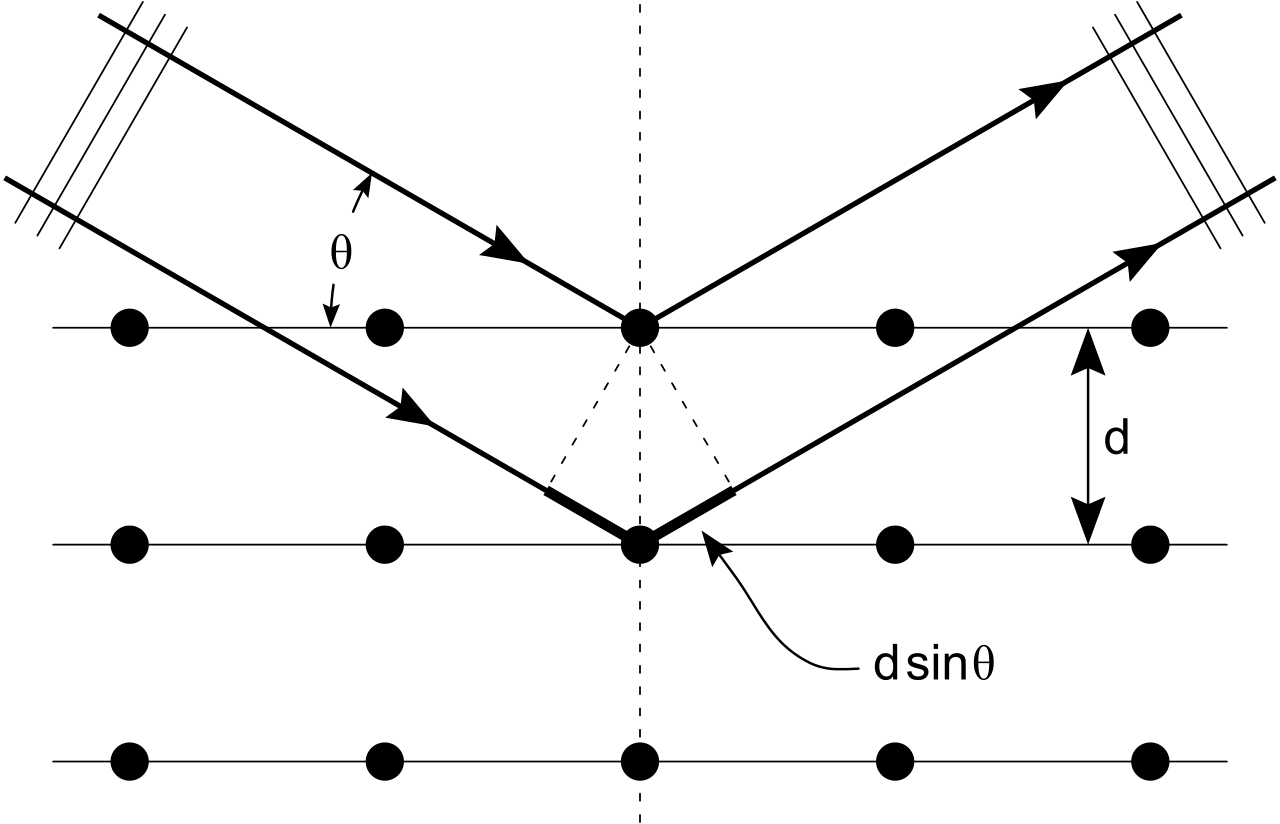
\includegraphics[width=0.5\linewidth]{Figures/Bragg_diffraction_2.svg.png}
    \caption{Bragg diffraction: Two beams with identical wavelength and phase approach a crystalline solid and are scattered off two different atoms within it. The lower beam traverses an extra length of $2d\sin\theta$. Constructive interference occurs when this length is equal to an integer multiple of the wavelength of the radiation \cite{wikipediacontributors_2019_braggs}.}
    \label{fig:enter-label}
\end{figure}

\pagebreak{}

\subsection{Lattice Spacing and Constants of the 7 Crystal systems}

In subsection [\ref{subsection:CrystalSystems}], we discussed the concept of miller indices, and how they can specify orientations of
crystal planes in a lattice. So, it is no surprise that the lattice spacing of a crystal can be calculated using the miller indices of a plane, in addition to the lattice constants of the crystal. The equations for all 7 crystal systems are
shown in Appendix [\ref{appendix:Equations}].

\begin{figure}[h]
	\centering
	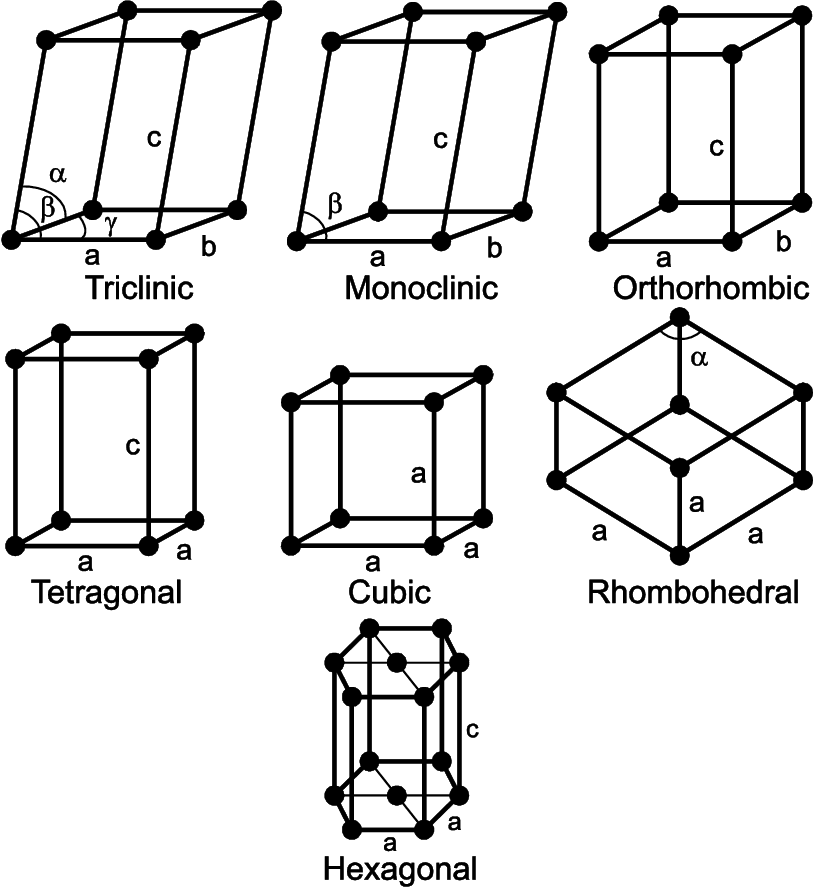
\includegraphics[width=0.5\textwidth]{Figures/UnitCells.png}
	\caption{The 7 crystal systems. \cite{shirokanev_2019_the}}
	\label{fig:crystalsystems}
\end{figure}

\subsection{Penetration Depth of X-rays}

Incident X-Rays on a sample are absorbed by the material, and the intensity of the transmitted X-Rays will intuitively decrease as the depth of the material increases. 
Therefore, knowing penetration depth is crucial in choosing sample dimensions. The absorption fraction $A(x)$ is expressed in terms of the linear absorption coefficient $\mu$ (used in [\ref{eq:absorption}]) and the depth $x$ as follows:

\begin{equation}
	A(x) = 1 - e^{-\mu x \left( \frac{1}{\sin\omega} + \frac{1}{\sin 2\theta - \omega} \right)}
\end{equation}

where $x$ is the distance the X-rays have traveled through the material, $\theta$ is the diffraction angle, and $\omega$ is the angle of incidence.

Also, the penetration depth $d$ is the depth in the material at which the intensity of the X-rays is reduced to $1/e$ or $~ 37\%$ of the initial intensity. This is given by:

\begin{equation}
	d = \left(\frac{\mu}{\sin\omega} + \frac{\mu}{\sin 2\theta - \omega}\right)^{-1}
\end{equation}

The following table shows the penetration depths of X-rays in various materials:


\begin{table}[h]
	\centering
	\begin{tabular}{|c|c|cc|cc|cc|}
	\hline
	\multirow{2}{*}{\textbf{Element (Z)}} &
	  \multirow{2}{*}{\textbf{Density ($\rho$) {[}g/cm³{]}}} &
	  \multicolumn{2}{c|}{\textbf{Co}} &
	  \multicolumn{2}{c|}{\textbf{Cu}} &
	  \multicolumn{2}{c|}{\textbf{Mo}} \\ \cline{3-8} 
	 &
	   &
	  \multicolumn{1}{c|}{$\omega = 1^{\circ}$} &
	  $\omega = 15^{\circ}$ &
	  \multicolumn{1}{c|}{$\omega = 1^{\circ}$} &
	  $\omega = 15^{\circ}$ &
	  \multicolumn{1}{c|}{$\omega = 1^{\circ}$} &
	  $\omega = 15^{\circ}$ \\ \hline
	C (6)   & 2.27  & \multicolumn{1}{c|}{9.64}  & 17.37 & \multicolumn{1}{c|}{15.35} & 117.9 & \multicolumn{1}{c|}{169.2} & 1300  \\ \hline
	Al (13) & 2.70  & \multicolumn{1}{c|}{0.83}  & 6.38  & \multicolumn{1}{c|}{1.29}  & 9.91  & \multicolumn{1}{c|}{12.70} & 97.9  \\ \hline
	Si (14) & 2.33  & \multicolumn{1}{c|}{0.77}  & 5.95  & \multicolumn{1}{c|}{1.20}  & 9.23  & \multicolumn{1}{c|}{11.75} & 90.3  \\ \hline
	Fe (26) & 7.86  & \multicolumn{1}{c|}{0.38}  & 2.89  & \multicolumn{1}{c|}{0.067} & 0.52  & \multicolumn{1}{c|}{0.58}  & 4.49  \\ \hline
	Cu (29) & 8.92  & \multicolumn{1}{c|}{0.24}  & 1.88  & \multicolumn{1}{c|}{0.37}  & 2.82  & \multicolumn{1}{c|}{0.39}  & 2.89  \\ \hline
	Zn (30) & 7.14  & \multicolumn{1}{c|}{0.28}  & 2.13  & \multicolumn{1}{c|}{0.42}  & 3.21  & \multicolumn{1}{c|}{0.45}  & 3.43  \\ \hline
	Zr (40) & 6.51  & \multicolumn{1}{c|}{0.12}  & 0.99  & \multicolumn{1}{c|}{0.19}  & 1.48  & \multicolumn{1}{c|}{1.60}  & 12.31 \\ \hline
	W (74)  & 19.25 & \multicolumn{1}{c|}{0.035} & 0.27  & \multicolumn{1}{c|}{0.052} & 0.40  & \multicolumn{1}{c|}{0.092} & 0.70  \\ \hline
	\end{tabular}
	\label{tab:penetrationdepth}
	\caption{Penetration depth ($\mu$) of elements subjected to Cobalt (Co), Copper (Cu), and Molybdenum (Mo) X-rays at different angles ($\omega$) of incidence. All values are in $\mu$m, and the absorption is $63 \%$. \cite{lotharspie_2019_moderne}}
\end{table}



\pagebreak{}

\subsection{Structure of polycrystalline samples and heteroepitaxial thin films}

Single crystals develop under specific conditions, whereas the usual solid state of an element or compound is polycrystalline. As implied by the term, a polycrystalline solid, or polycrystal, consists of numerous crystals. The characteristics of a polycrystal differ significantly from those of a single crystal. The individual crystals within a polycrystal are commonly called grains, 
and the interfaces between these grains are referred to as grain boundaries. These grains are randomly oriented, with different sizes and shapes. In [\ref{subsection:Task1}], we used a bulk polycrystalline sample of Si and ZnO. However, in [\ref{subsection:Task2}], we used thin films of ZnO grown on sapphire substrates; a heteroepitaxial thin film. 

Heteroepitaxy is a process in which a thin film is grown on a substrate with a different lattice constant. The lattice mismatch between the film and the substrate can be quantified using the equation:

\begin{equation}
	\label{eq:latticemismatch}
	\frac{\Delta a}{a} = \frac{a_{\text{substrate}} - a_{\text{film}}}{a_{\text{substrate}}}
\end{equation}

If this lattice mismatch is small enough, the film can grow in a \textit{psuedomorphic} fashion; where it tries to match the lattice constant of the substrate. The figure below illustrates said process:

\begin{figure}[h]
	\centering
	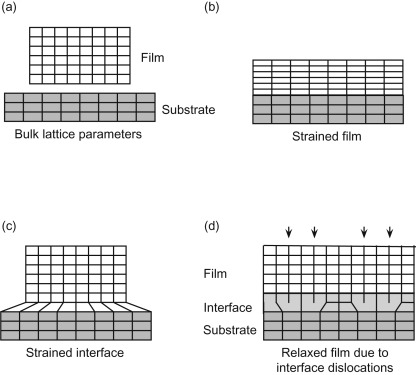
\includegraphics[width=0.5\textwidth]{Figures/Heteroepitaxy.jpg}
	\caption{(a) Schematic of bulk lattice parameters, or atomic spacings, of the film and substrate materials if they were not constrained in any way. (b) Typical strain in a film, where the entire film is constrained by the substrate, which is much thicker than the film. This is psuedomorphic growth (c) An unusual case where all of the strain is at the interface, for example when mechanically soft layers are used for compliance at the interface. d) A relaxed film where dislocations form between the film and substrate (below the arrows shown) to minimize the strain in the film. \cite{buschow_2001_encyclopedia}}
	\label{fig:epitaxy}
\end{figure}

The film undergoes a volumetric strain that accumulates with each added layer until it reaches a critical thickness. When the thickness exceeds this critical point, the elastic strain in the film is alleviated by the creation of dislocations.
These dislocation are classified into two types: edge and screw dislocations. Mathmetically, these disclocations can be described via the use of the Burgers vector. By moving in a 360$^{\circ}$ loop around the dislocation, there will be difference in the starting point and the end point, which is the Burgers vector. This is illustrated below:

\begin{figure}[h]
	\centering
	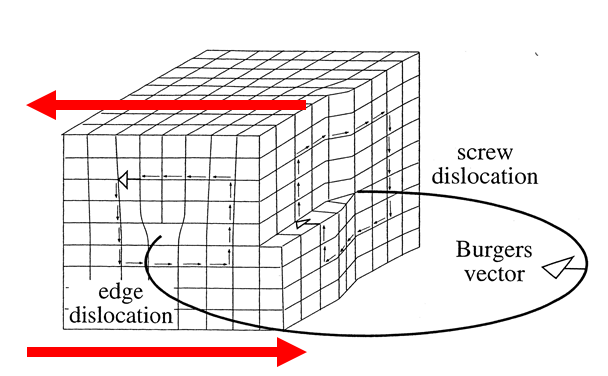
\includegraphics[width=0.4\textwidth]{Figures/dislocation.png}
	\caption{The Figure shows both edge and screw dislocations in an indealized cubic lattice. The edge dislocation is on the front face and the screw dislocation is on the right face. Burgers vectors are denoted with white-tipped arrows, and point in the same direction for the two dislocations shown. Red arrows indicate applied shear. \cite{passchier_2013_microtectonics} \cite{_2016_relation}}
	\label{fig:burgersvector}
\end{figure}

Dislocations naturally arrange themselves into the most stable configurations to achieve thermodynamic stability; edge-type dislocations typically group together. 
These clusters are called grain boundaries and represent two-dimensional defects that mark the borders between two monocrystalline regions, or crystallites, which are rotated relative to each other.
Edge-type dislocations generally cause a twist in the crystallites and screw-type dislocations can result in a tilt.

\pagebreak{}

\subsection{Errors in goniometer measurement and methods for elimination of errors}

Our X-Ray machine looks like the following:

\begin{figure}[h]
	\centering
	\includegraphics[width=0.5\textwidth]{Figures/Diffractometer.jpg}
	\caption{Main components of the X-Ray Diffractometer.}
	\label{fig:xraymachine}
\end{figure}

To determine the lattice constants, what we measure in the experiment is $\theta$. But, what we need for interplanar distances and miller indices is Bragg's law, which is in terms of $\sin \theta$.
Meaning the precision of the lattice constants is dependent on $\sin \theta$. This is actually advantageous as values of $\theta$ closer to 90$^{\circ}$ will have higher precision, as shown below:

\begin{figure}[h]
	\centering
	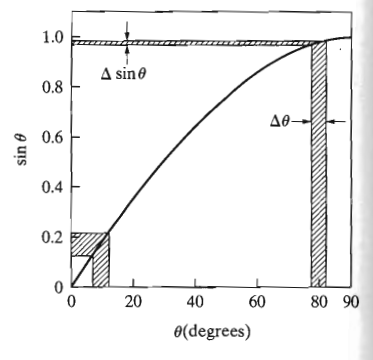
\includegraphics[width=0.3\textwidth]{Figures/sintheta.png}
	\caption{The relationship between $\sin \theta$ and $\theta$.}
	\label{fig:sintheta}
\end{figure}

So, by differentating braggs law one can see that:

\begin{equation}
	\label{eq:error1}
	\frac{\Delta d}{d} = \frac{\Delta \lambda}{\lambda} - \cot \theta \Delta \theta
\end{equation}

Using the equation for a cubic system in [\ref{appendix:Equations}], and ignoring $\lambda$:

\begin{equation}
	\label{eq:error2}
	\frac{\Delta a}{a}= \frac{\Delta d}{d} = -cot \theta \Delta \theta
\end{equation}

The main sources of error in goniometer measurements are:

\begin{enumerate}
    \item \textbf{Instrument misalignment.} Specifically, the incident beam's center must align with the diffractometer axis and the 0° position of the detector slit.
    \item \textbf{Use of a flat specimen instead of one that conforms to the focusing circle.} To minimize this error, despite a reduction in intensity, decrease the specimen's irradiated width using an incident beam with minimal horizontal divergence.
    \item \textbf{Specimen absorption.} Thin specimens with low absorption are preferable.
    \item \textbf{Specimen displacement from the diffractometer axis ([\ref{fig:peakshift}]).} This is often the largest single source of error, causing an error in \(d\) as given by:
       \[
       \frac{\Delta d}{d} = -\frac{D \cos^2 \theta}{R \sin \theta}
       \]
       where \(D\) is the specimen displacement parallel to the diffraction-plane normal (positive when the displacement is in front of the axis) and \(R\) is the diffractometer radius.
    \item \textbf{Vertical divergence of the incident beam.} Minimize this error, despite a reduction in intensity, by adjusting the detector slit to reduce the vertical opening.
\end{enumerate}

\pagebreak{}

\begin{figure}[h]
	\centering
	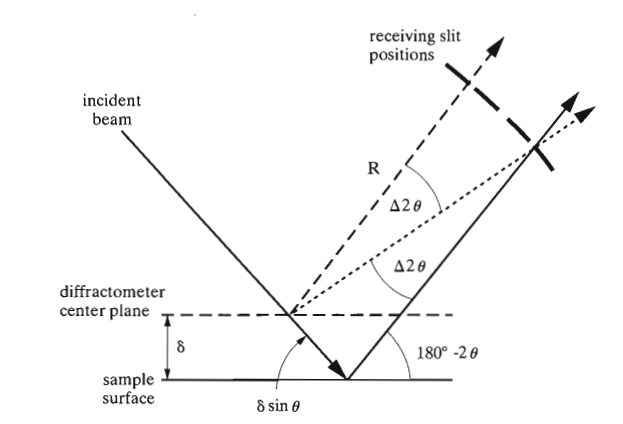
\includegraphics[width=0.4\textwidth]{Figures/peakshift.png}
	\caption{Shift of peak position due to sample displacement}
	\label{fig:peakshift}
\end{figure}

for errors (2) and (3):

\begin{equation}
	\label{eq:error1}
	\frac{\Delta d}{d} = \cos^2 \theta
\end{equation}

for error (4):

\begin{equation}
	\label{eq:error4}
	\frac{\Delta d}{d} = \frac{\cos^2 \theta}{\sin \theta}
\end{equation}

Often, the effect of (5) is included in the extrapolation function such that:
 
\begin{equation}
	\label{eq:error3}
	\frac{\Delta d}{d} = \frac{\cos^2 \theta}{\sin \theta} + \frac{\cos^2 \theta}{\theta}
\end{equation}

This is is termed the Nelson-Riley function. \cite{bernarddeniscullity_2015_elements}

So, using [\ref{eq:error1}], [\ref{eq:error2}], [\ref{eq:error3}], one can fit for the lattice parameters using:

\begin{align*}
	\label{eq:fit}
	\frac{\Delta a}{a_0} &= \frac{\Delta d}{d} = f_{\text{error}}(\theta)
	\rightarrow a = a_0 + a_0 \cdot f_{\text{error}}(\theta)
\end{align*}
\pagebreak{}

\section{Analysis}

\subsection{Task 1}
\label{subsection:Task1}

In task 1, we measured the XRD diffraction patterns of Si and ZnO in 2$\theta$ - $\omega$ mode.

\subsubsection{Bragg Peaks}

\begin{figure}[h]
	\centering
	\begin{subfigure}{\textwidth}
		\centering
		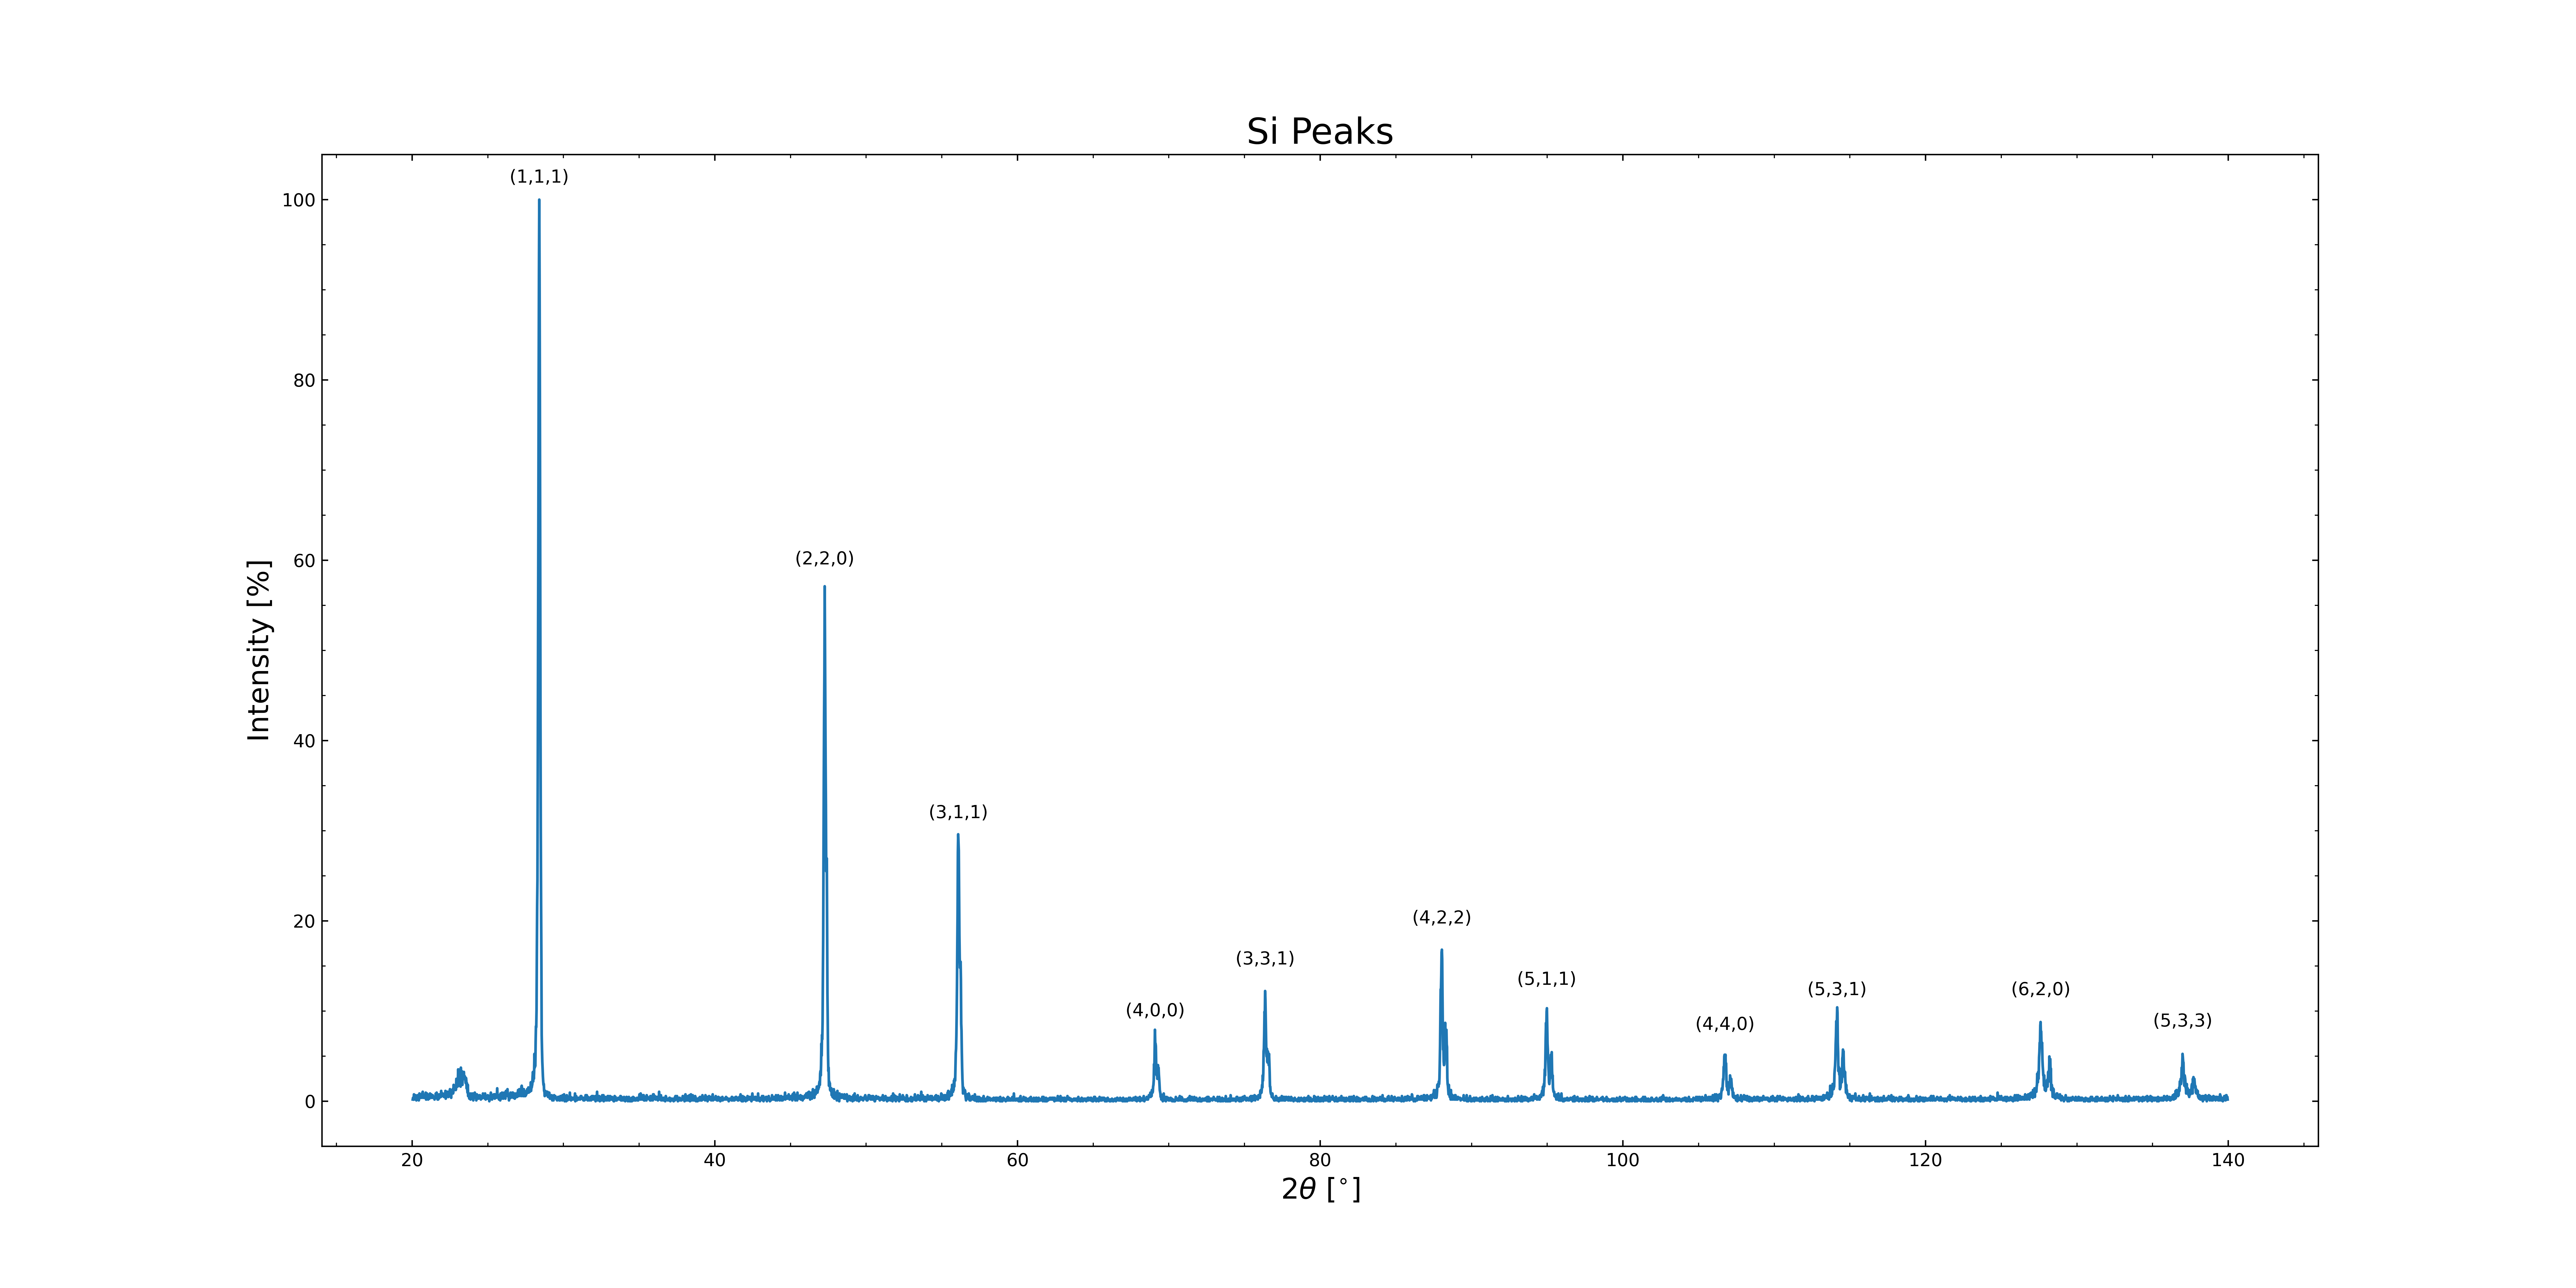
\includegraphics[width=0.7\textwidth]{Figures/SiPeaks.png}
		\caption{Si Bragg peaks labelled by miller indices acquired from the PC-PDF database.}
		\label{fig:SiPeaks}
	\end{subfigure}

	\begin{subfigure}{\textwidth}
		\centering
		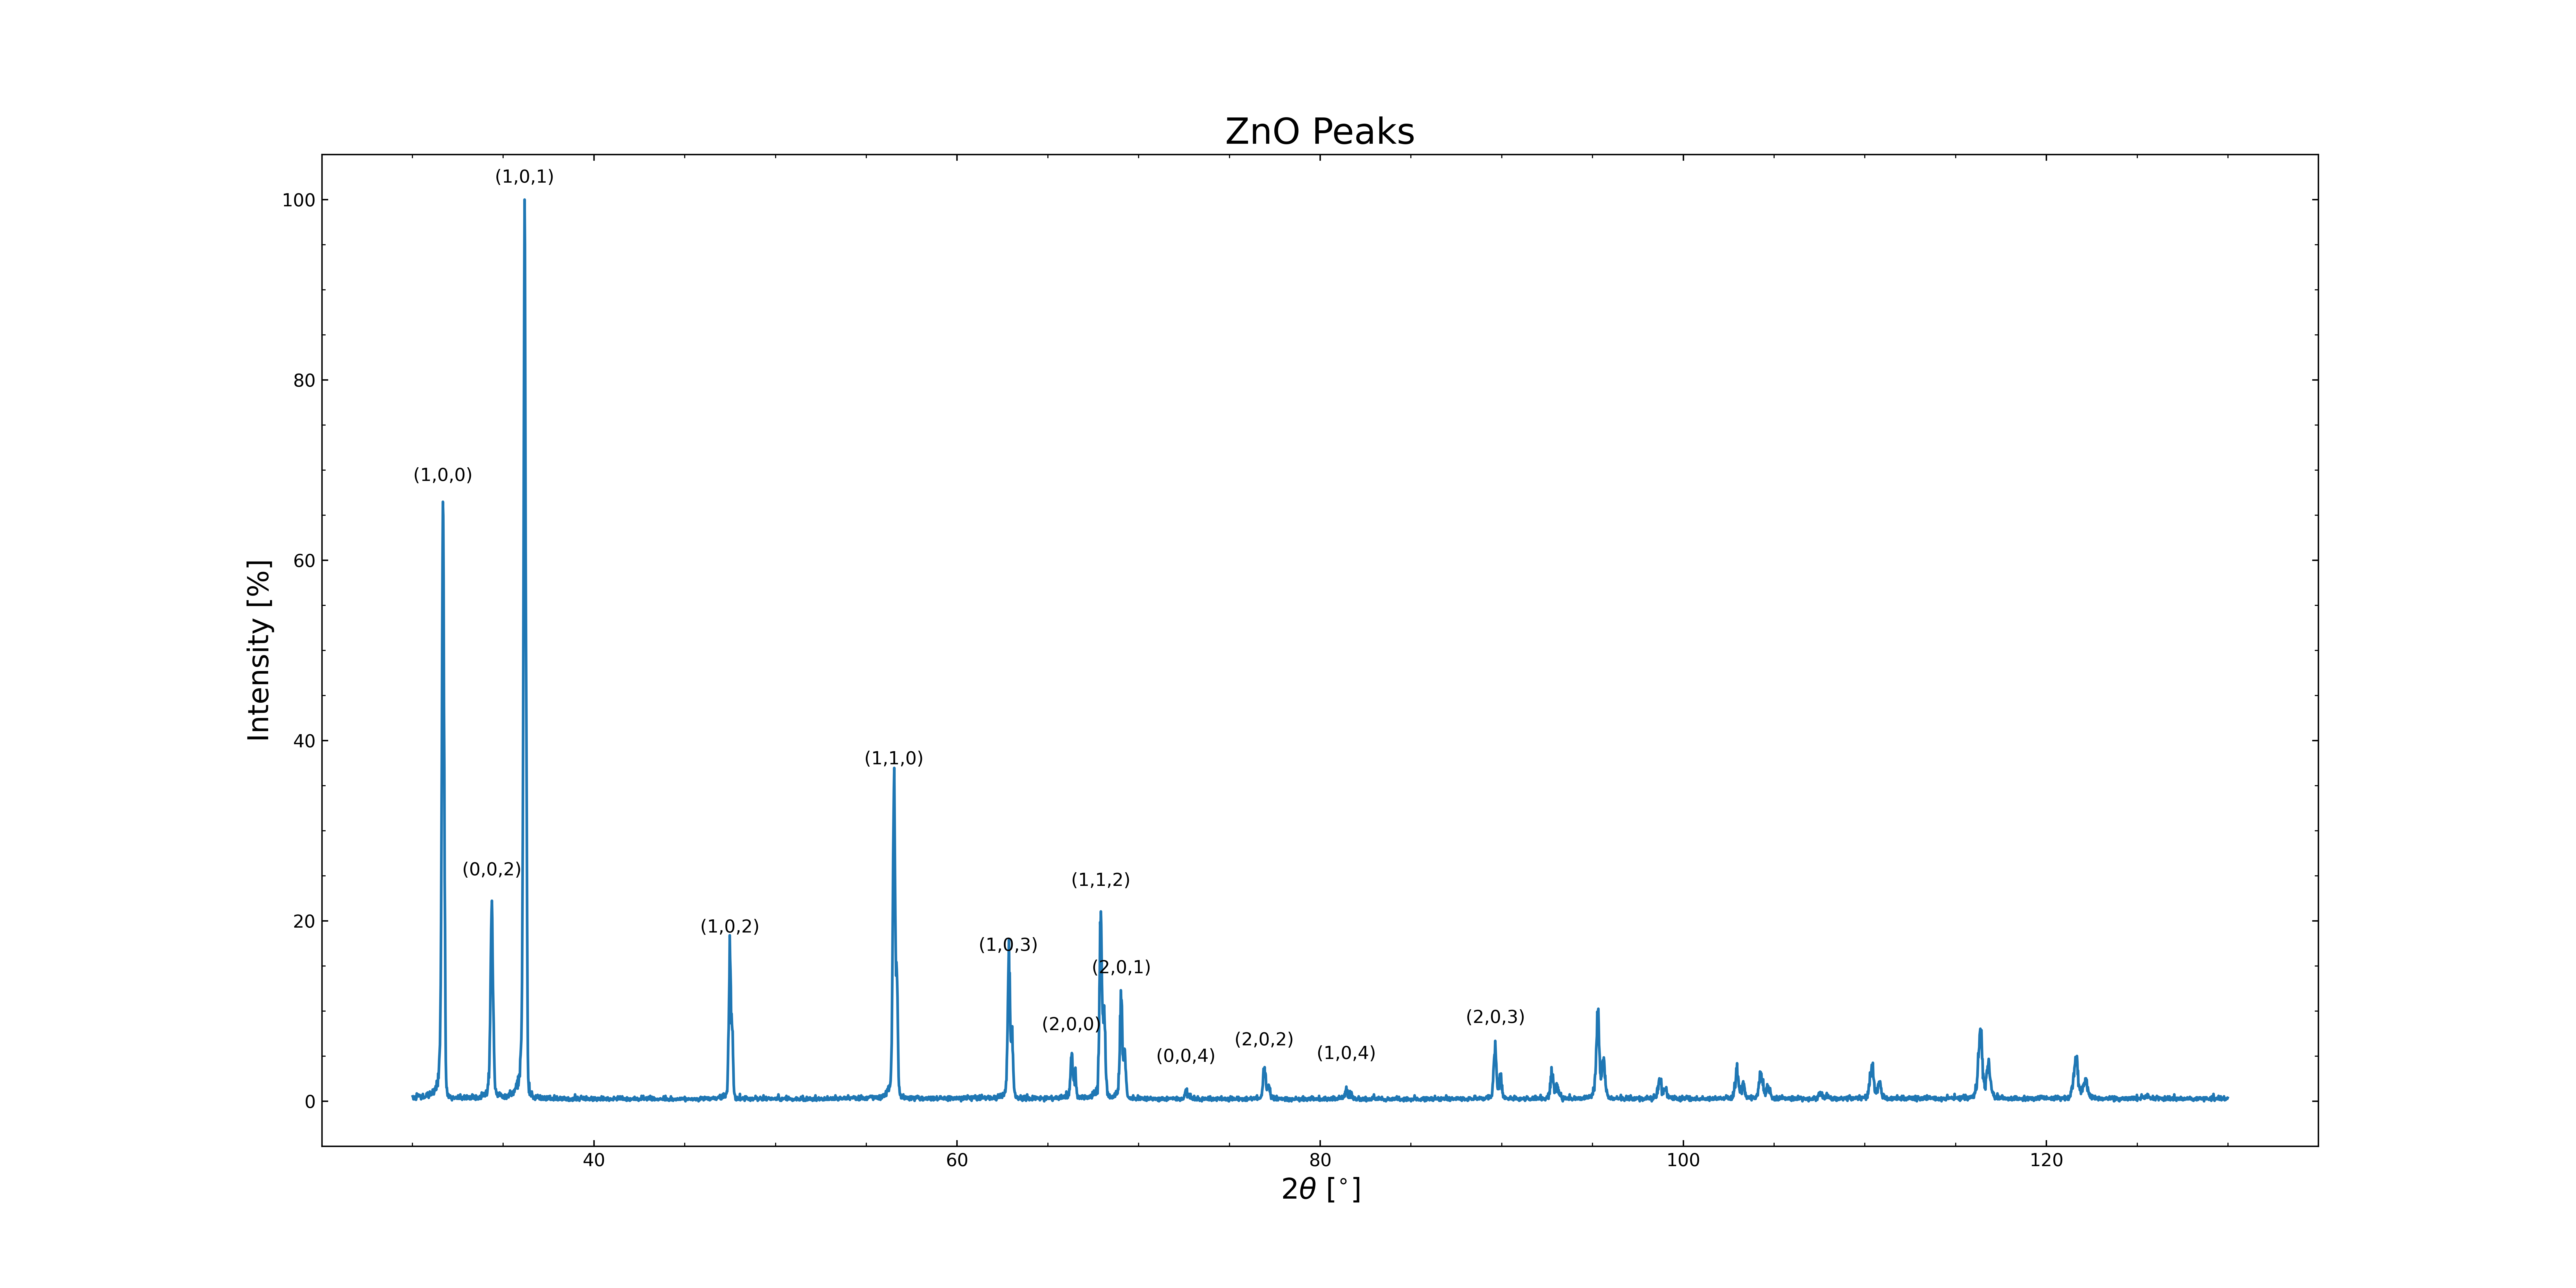
\includegraphics[width=0.7\textwidth]{Figures/ZnOPeaks.png}
		\caption{ZnO Bragg peaks labelled by miller indices acquired from the PC-PDF database.}
		\label{fig:ZnOPeaks}
	\end{subfigure}
	\caption{Bragg peaks of Si and ZnO.}
	\label{fig:BraggPeaks}
\end{figure}


The peaks in Figure [\ref{fig:SiPeaks}] were found by matching the $ 2 \theta $ values of the peaks from the PC-PDF database with the peaks in the XRD pattern. 
The peaks matched well, but some peaks were not present in the PC-PDF file (notably the one in the beginning), and hence were not labelled.


	Similarly to Si, the peaks in Figure [\ref{fig:ZnOPeaks}] were found by matching the $ 2 \theta $ values of the peaks from the PC-PDF database with the peaks in the XRD pattern. 
Again, the peaks matched well, but some peaks were not present in the PC-PDF file (notably towards the end), and hence were not labelled.

\pagebreak{}

\subsubsection{Unit Cells}

\begin{figure}[h]
	\centering
	\begin {subfigure}{0.35\textwidth}
		\centering
		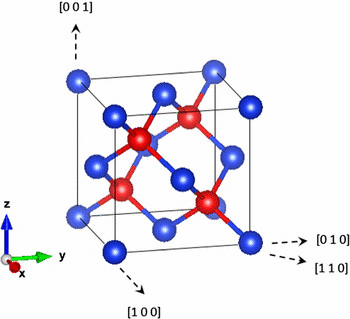
\includegraphics[width=0.9\textwidth]{Figures/SiUnitCell.png}
		\caption{Si unit cell. Red spheres are Si atoms from a different FCC lattice. \cite{samadi_2019_design}}
		\label{fig:SiUnitCell}
	\end{subfigure}
	\hfill
	\begin {subfigure}{0.6\textwidth}
		\centering
		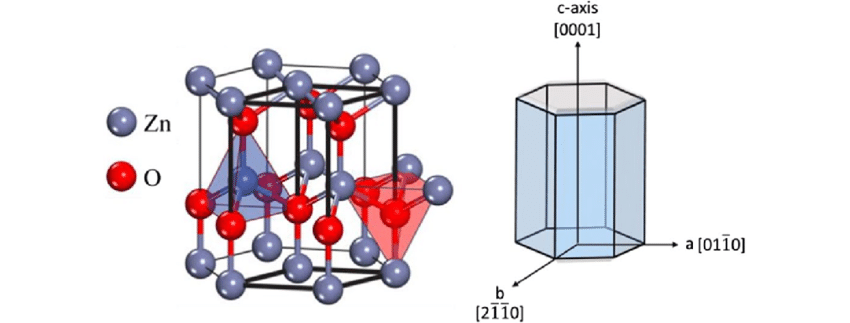
\includegraphics[width=\textwidth]{Figures/ZnOUnitCell.png}
		\caption{ZnO unit cell. \cite{urata_2016_higher}}
		\label{fig:ZnOUnitCell}
	\end{subfigure}
	\caption{Unit cells of Si and ZnO.}
	\label{fig:UnitCells}
\end{figure}

Si has a face-centered cubic (FCC) unit cell, as shown in Figure [\ref{fig:SiUnitCell}]. The lattice constant of Si was found to be $ \SI{5.4309}{\angstrom}$ by the PC-PDF database.
ZnO has a hexagonal wurzite unit cell, as shown in Figure [\ref{fig:ZnOUnitCell}]. The lattice constants of ZnO were found to be $a = \SI{3.2499}{\angstrom}$ and $c =  \SI{5.2066}{\angstrom}$ by the PC-PDF database.

For a cubic unit cell, the relation between the lattice constant $a$ and the $d$-spacing is given by equation [\ref{eq:cubic}]. This can be slightly modified using Braggs law (equation [\ref{eq:Bragg}]) to give equation:
\begin{equation}
	\label{eq:cubicmodified}
	d = \frac{\lambda \sqrt{h^2 + k^2 + l^2}}{2\sin(\theta)}
\end{equation}

We can do the same for a hexagonal unit cell, using equation [\ref{eq:hexagonal}] and Braggs law (equation [\ref{eq:Bragg}]) but under certain conditions to make the equation workable.

For $h=k=0$:
\begin{equation}
	\label{eq:hexmodified}
	d = \frac{\lambda l}{2\sin(\theta)}
\end{equation}

For $l=0$:
\begin{equation}
	\label{eq:hexmodified2}
	d = \frac{\lambda \sqrt{h^2 + hk + k^2}}{\sqrt{3}\sin(\theta)}
\end{equation}

This is done to find our experimental values of the lattice constants of Si and ZnO. Since we know $\lambda = \SI{1.54045}{\angstrom}$, and the angle $\theta$ is given in the data, then one could fit for the lattice parameters using 
the 3 error-correcting equations [\ref{eq:error1}], [\ref{eq:error2}], and [\ref{eq:error3}].

\pagebreak{}

\subsubsection{Fitting}

	For Si, the following 3 fits were done:

\begin{figure}[h]
	\centering
	\begin {subfigure}{0.3\textwidth}
		\centering
		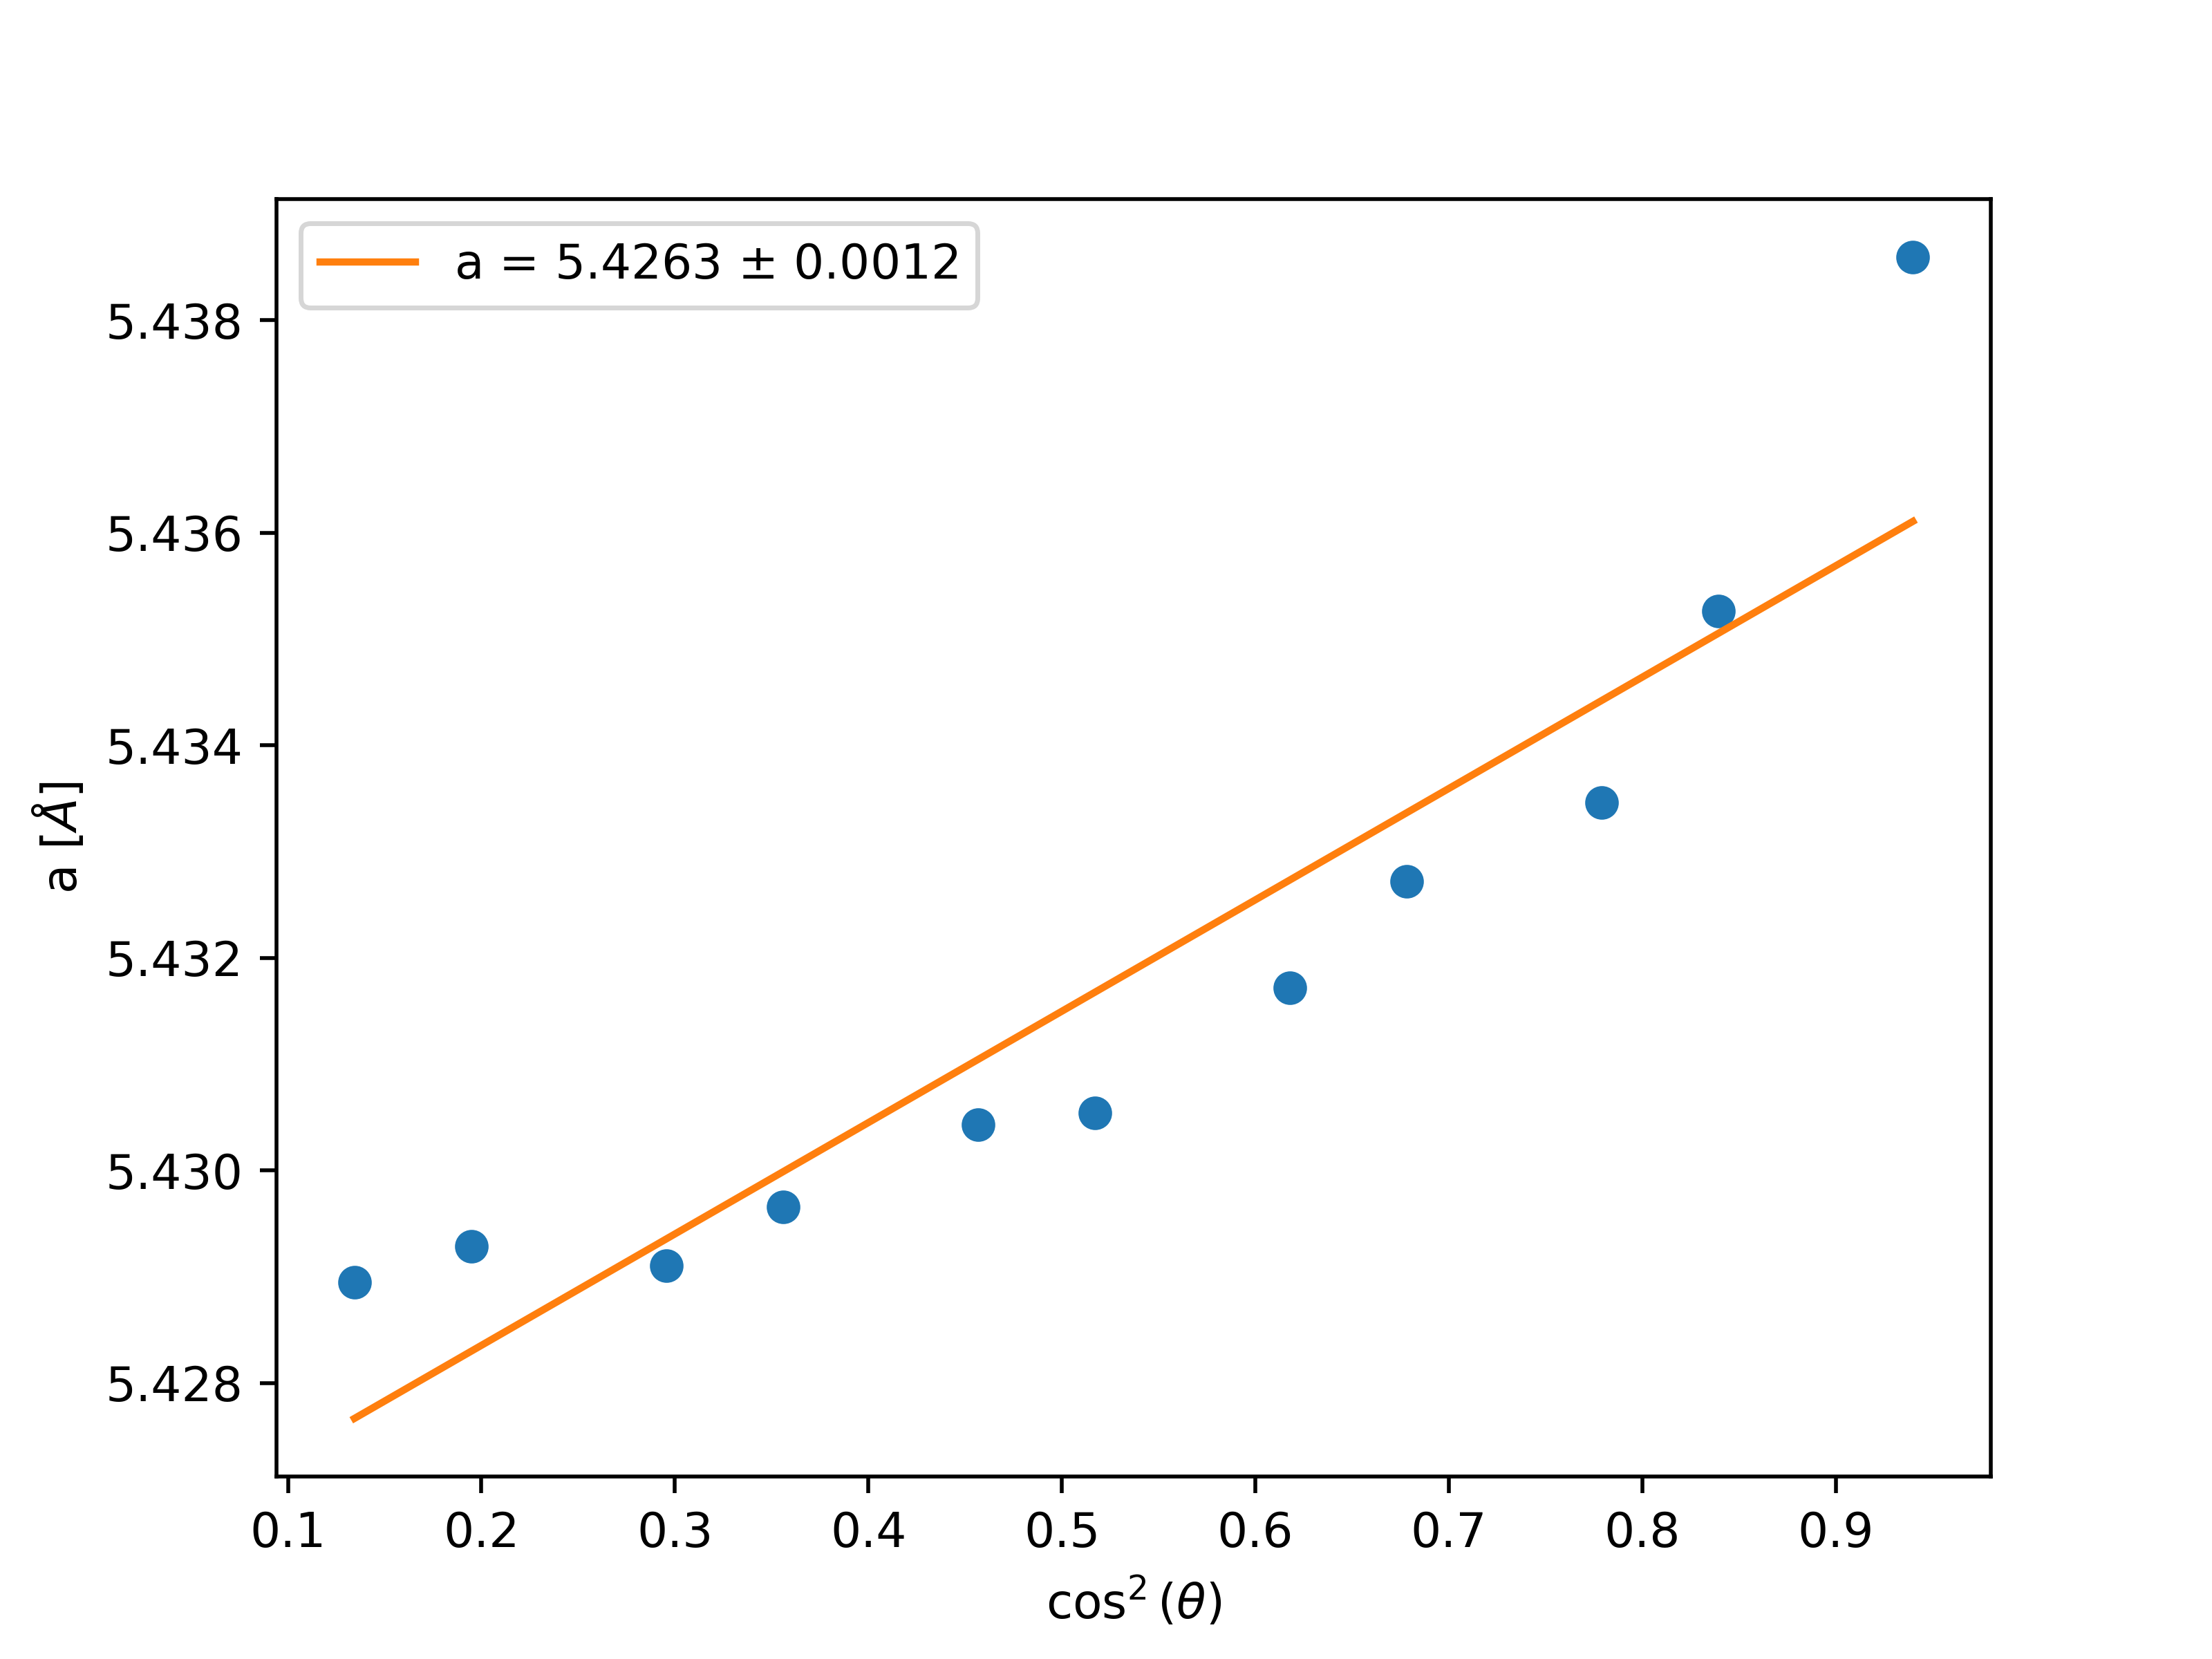
\includegraphics[width=\textwidth]{Figures/SiCos.png}
		\caption{Fit 1: $a=5.4263 \pm  \SI{0.0012}{\angstrom} $}
		\label{fig:SiFit1}
	\end{subfigure}
	\hfill
	\begin {subfigure}{0.3\textwidth}
		\centering
		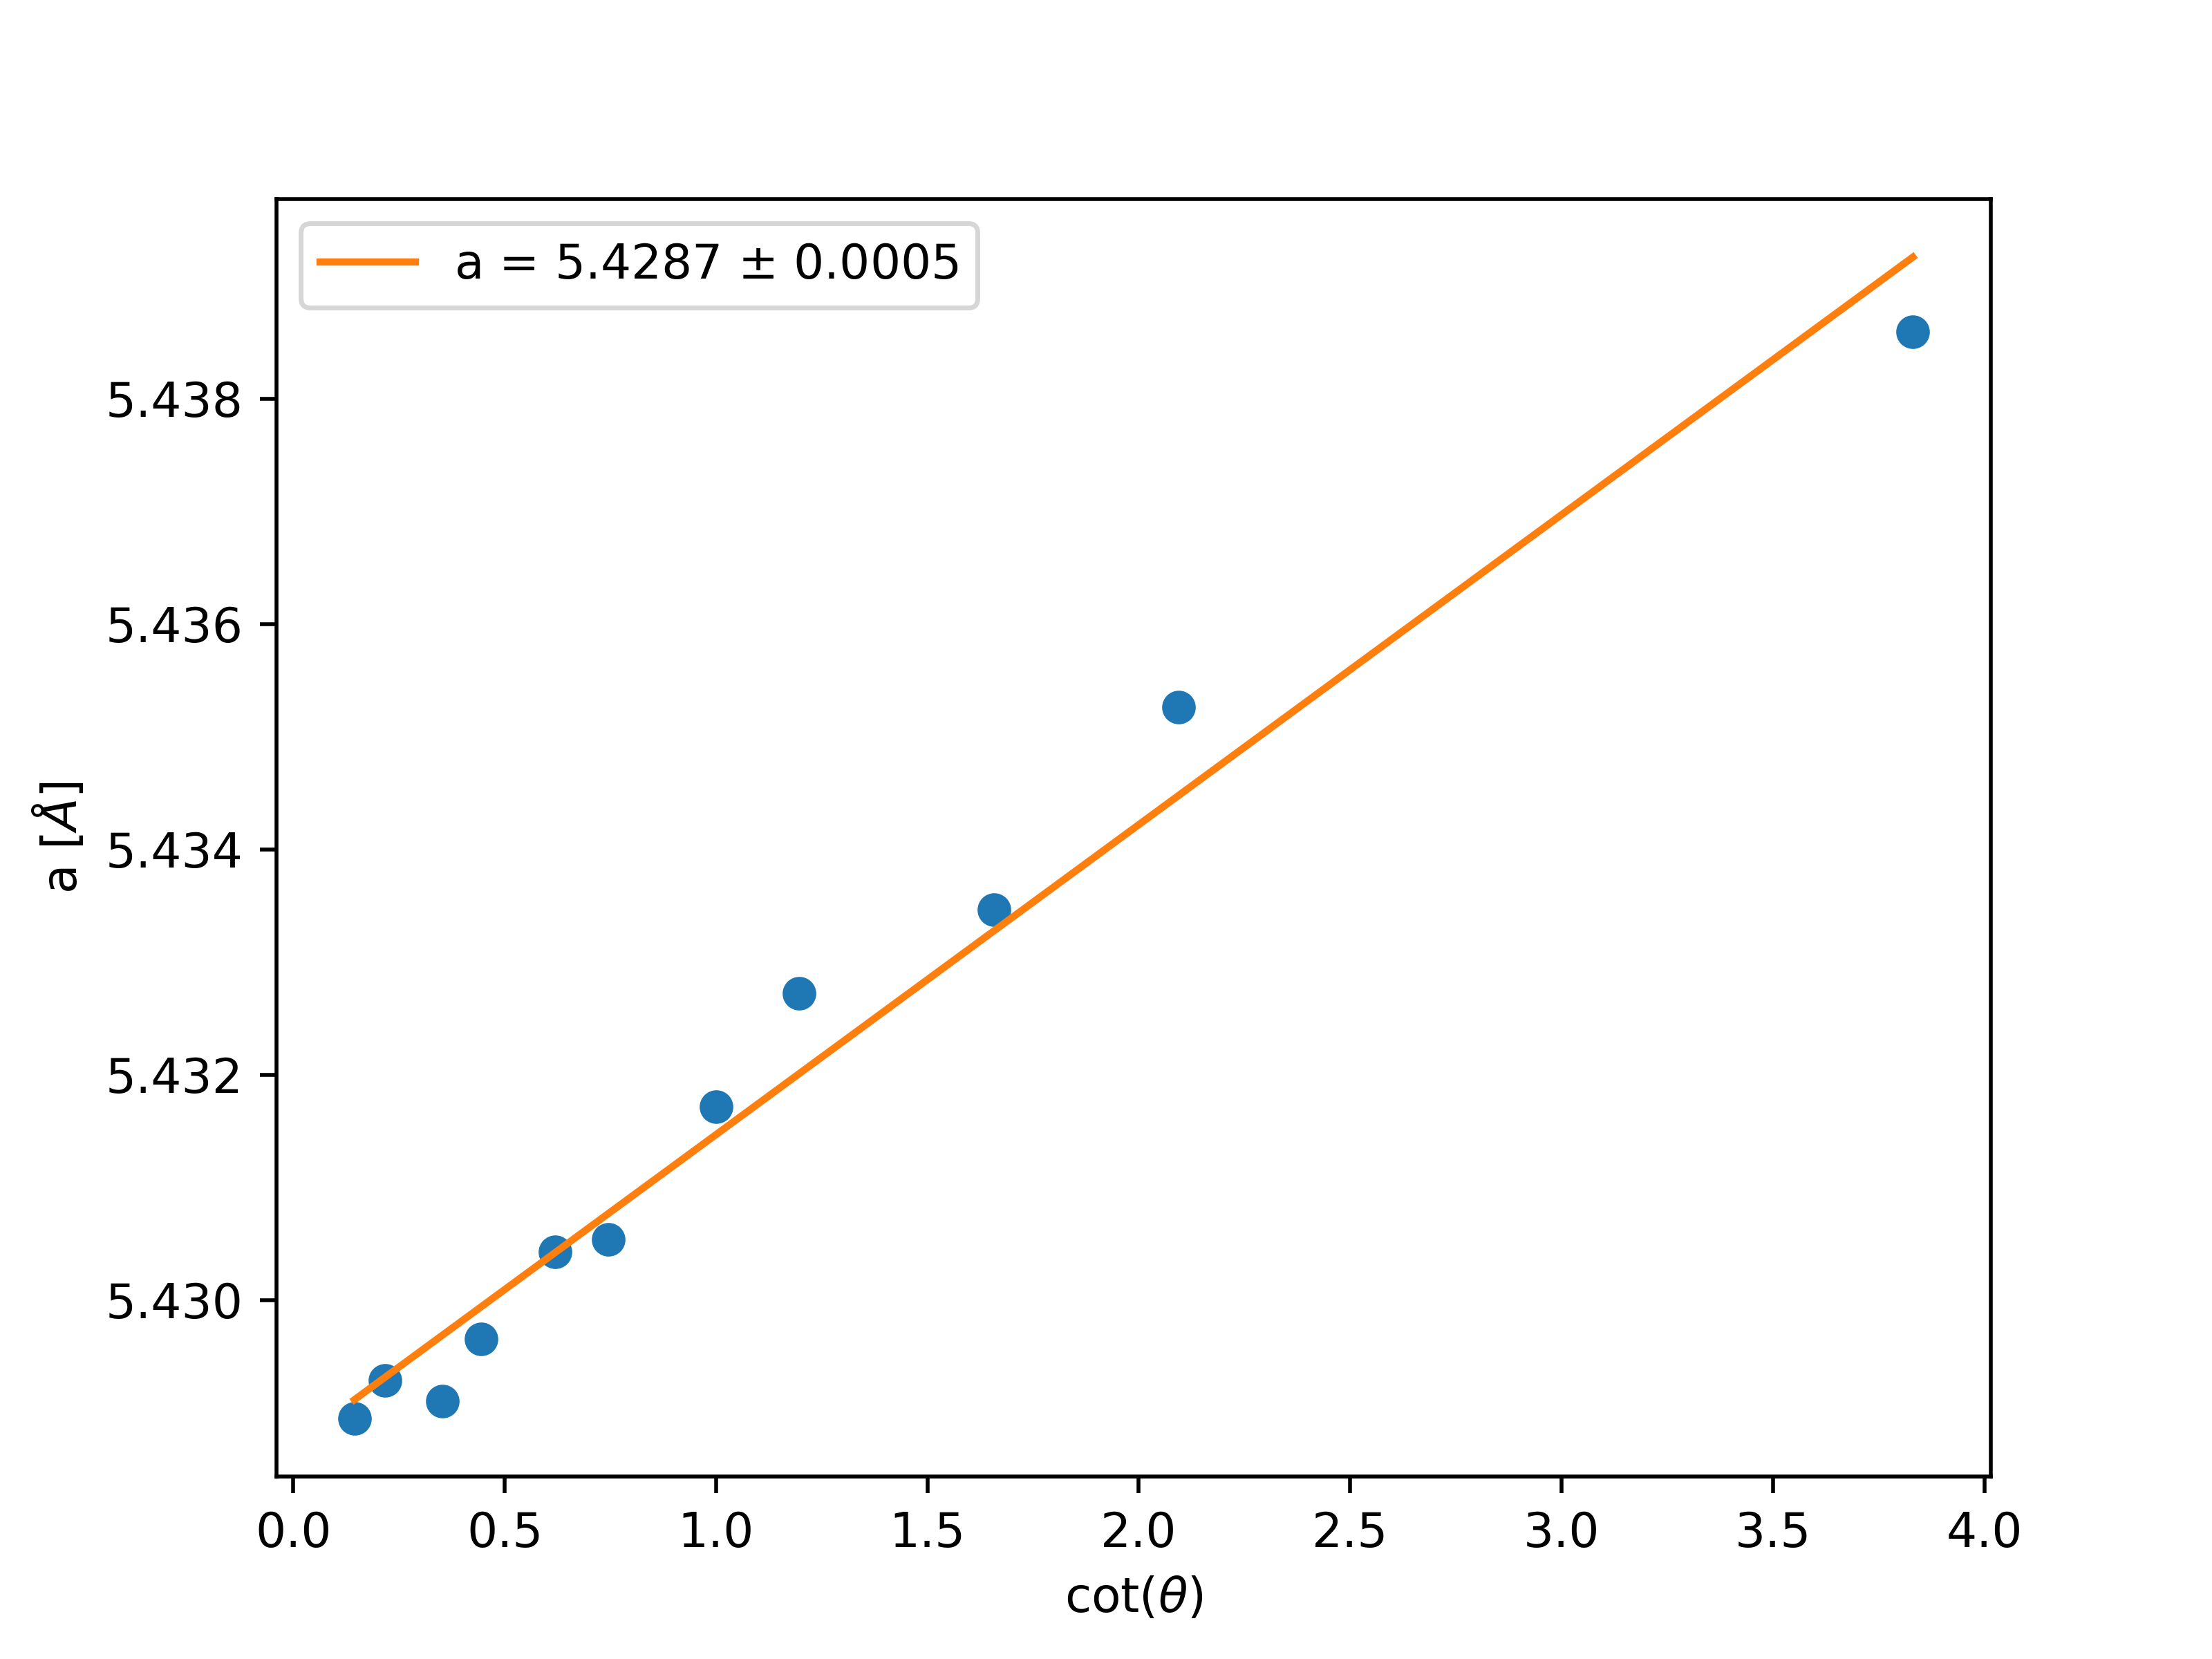
\includegraphics[width=\textwidth]{Figures/SiCot.png}
		\caption{Fit 2: $a=5.4287 \pm  \SI{0.0005}{\angstrom} $}
		\label{fig:SiFit2}
	\end{subfigure}
	\hfill
	\begin {subfigure}{0.3\textwidth}
		\centering
		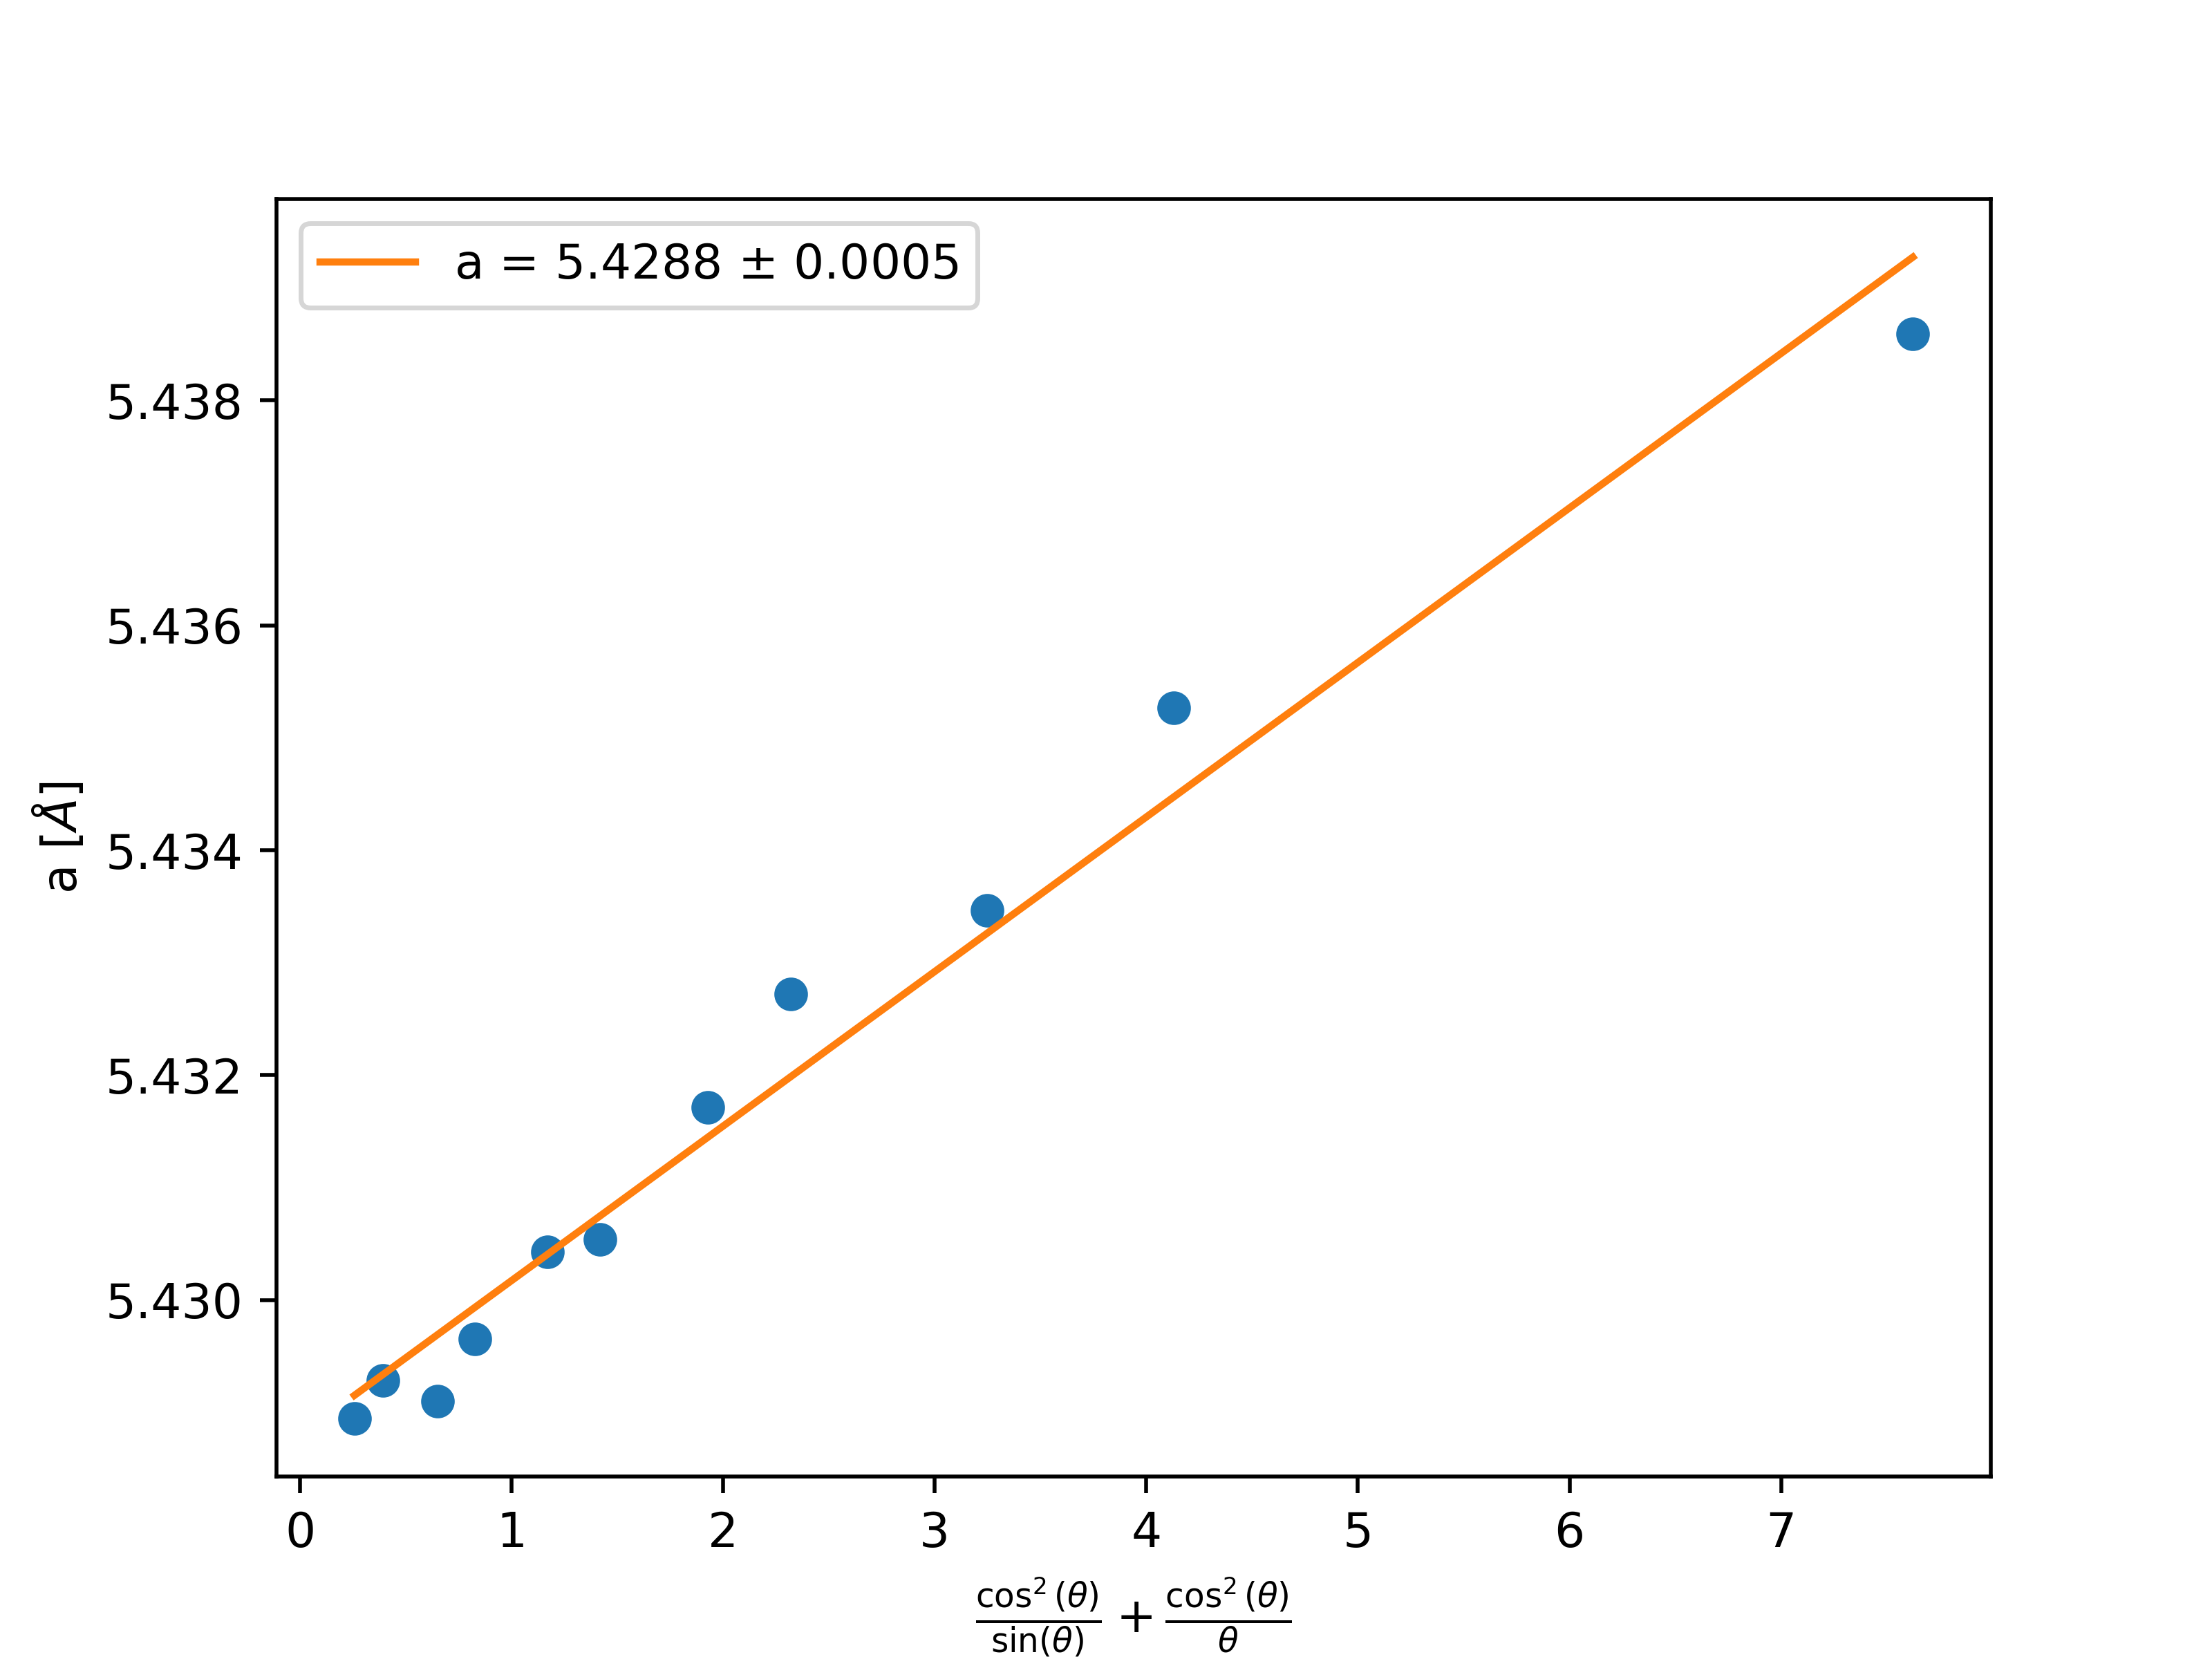
\includegraphics[width=\textwidth]{Figures/SiNelson.png}
		\caption{Fit 3: $a=5.4288 \pm  \SI{0.0005}{\angstrom} $}
		\label{fig:SiFit3}
	\end{subfigure}
	\caption{Fits for Si.}
	\label{fig:SiFits}
\end{figure}

The third fit against the Nelson-Riley function was the best fit, with the lattice constant being $~ 0.04 \%$ off from the PC-PDF value.



For ZnO, the following 6 fits were done:

\begin{figure}[h]
	\centering
	\begin {subfigure}{0.3\textwidth}
		\centering
		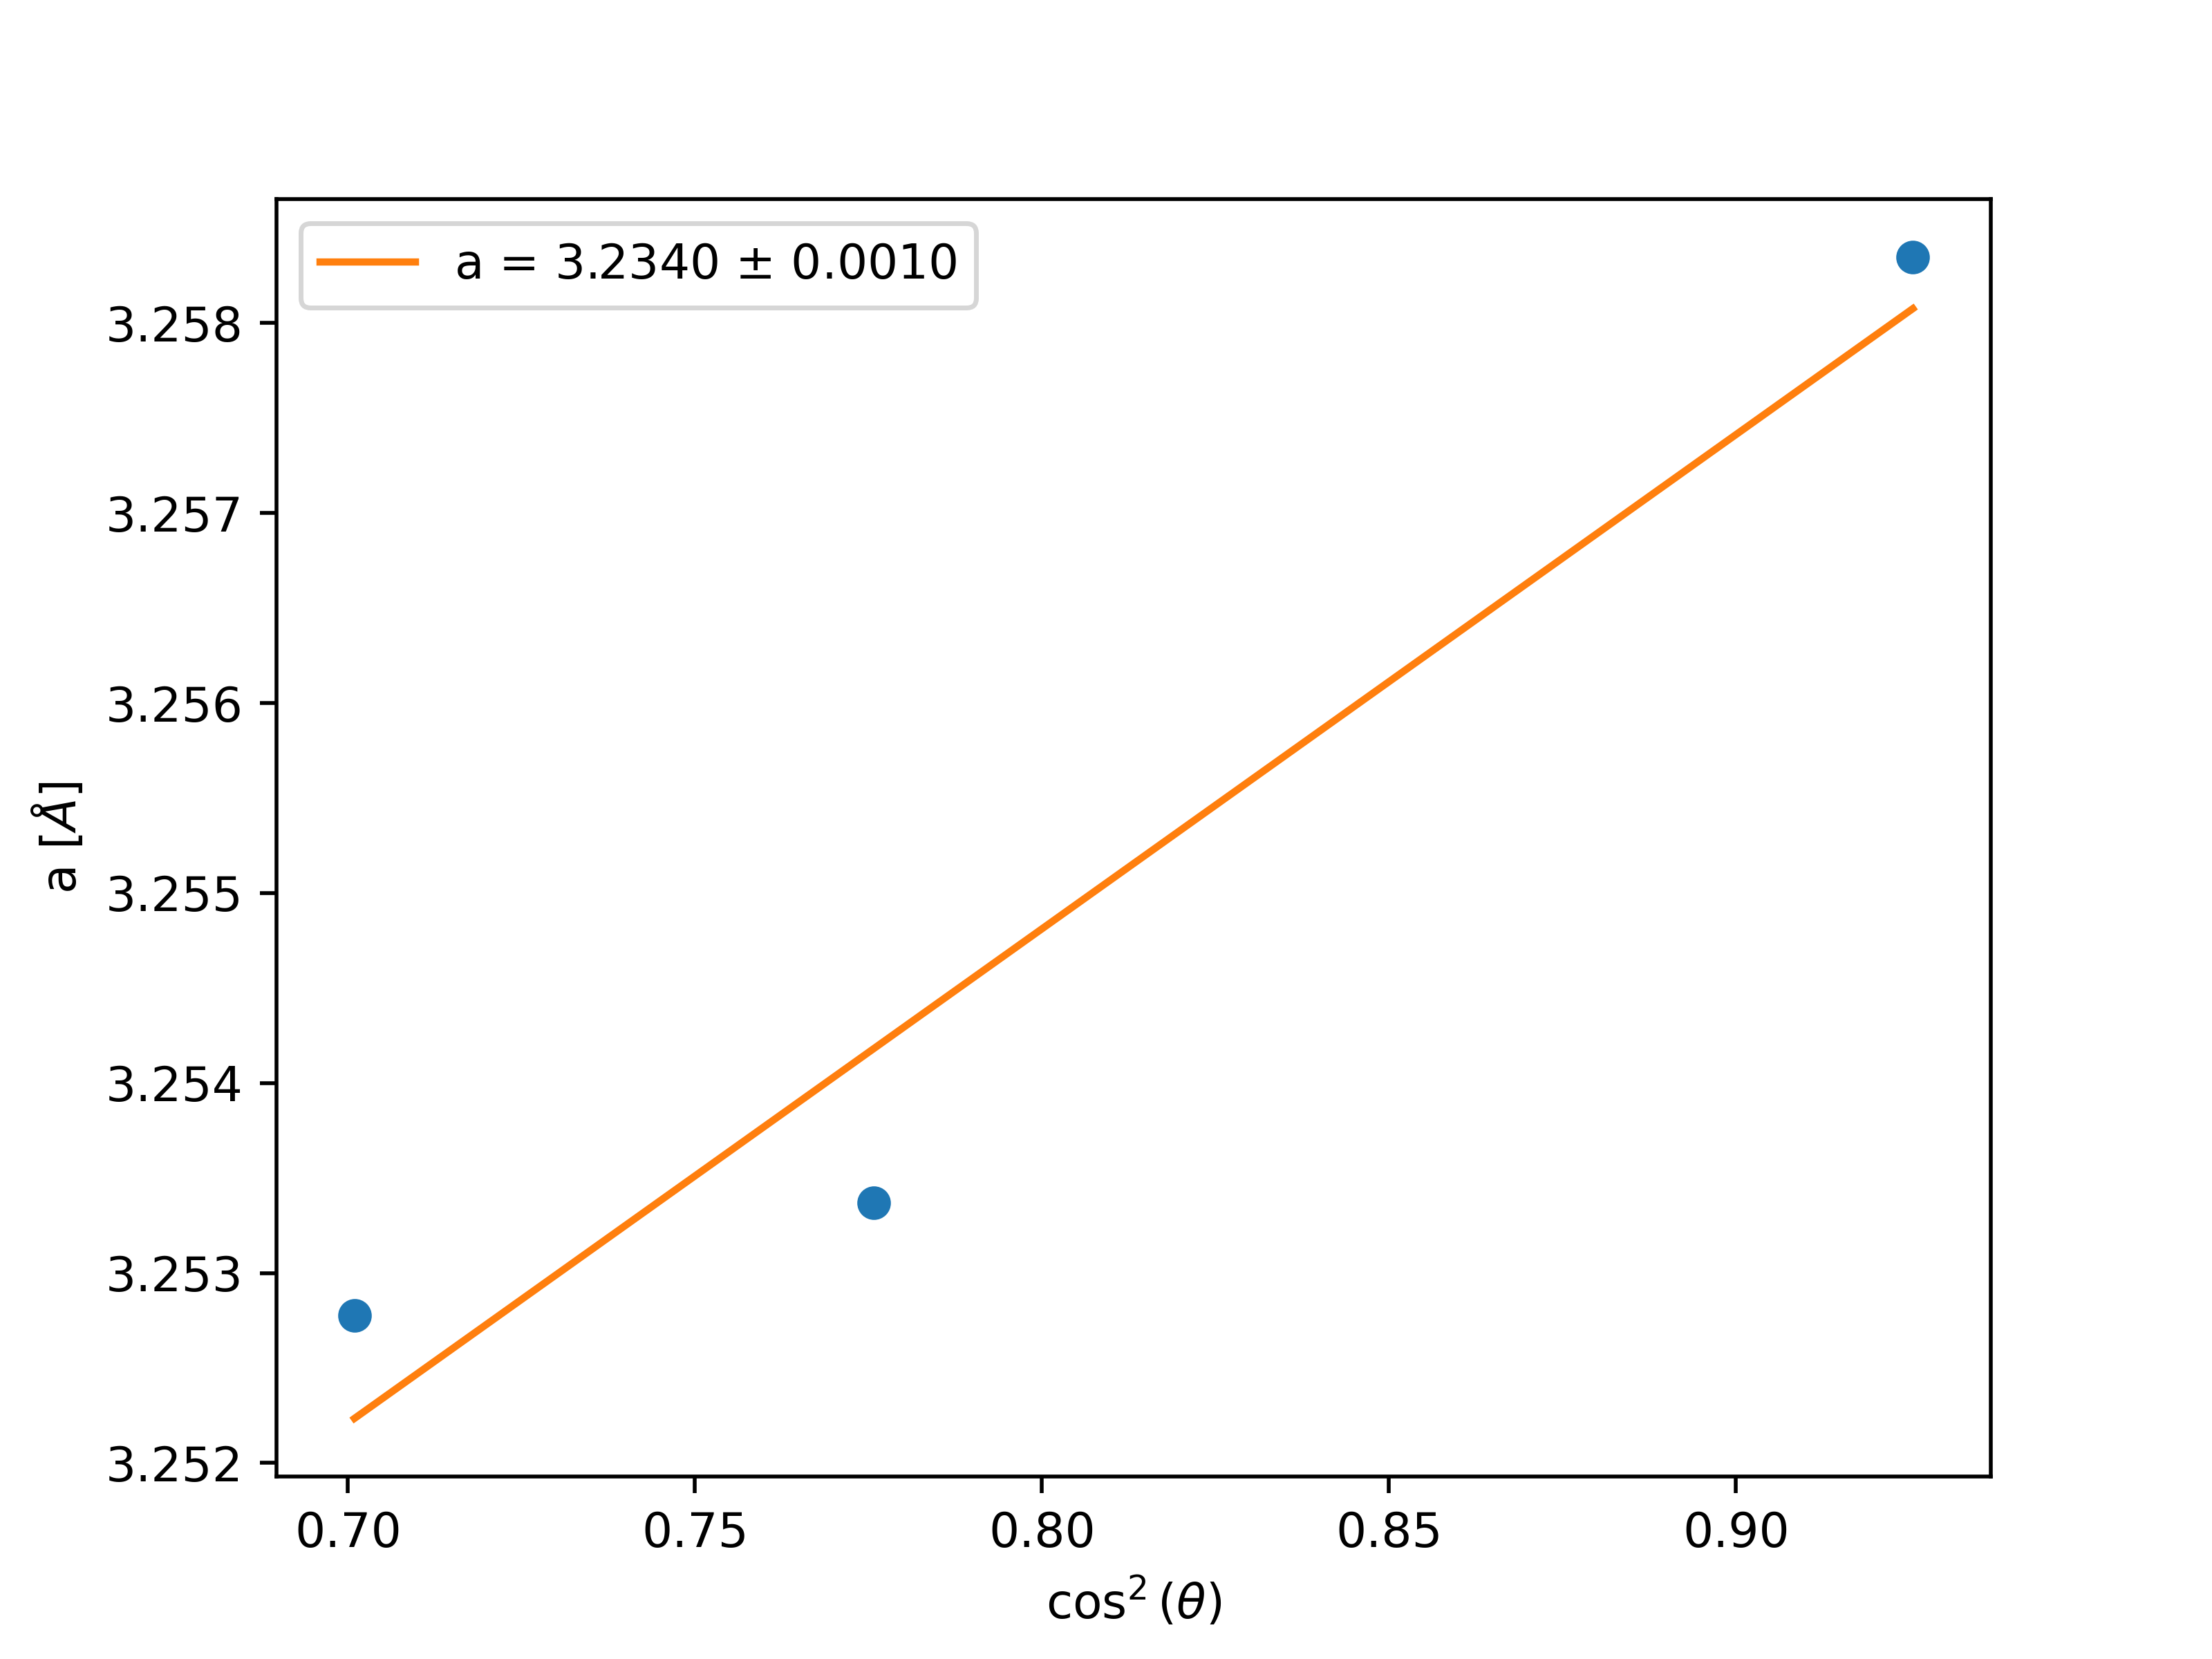
\includegraphics[width=\textwidth]{Figures/ZnOCosA.png}
		\caption{Fit 1: $a=3.2490 \pm \SI{0.0010}{\angstrom} $}
		\label{fig:ZnOFit1}
	\end{subfigure}
	\hfill
	\begin {subfigure}{0.3\textwidth}
		\centering
		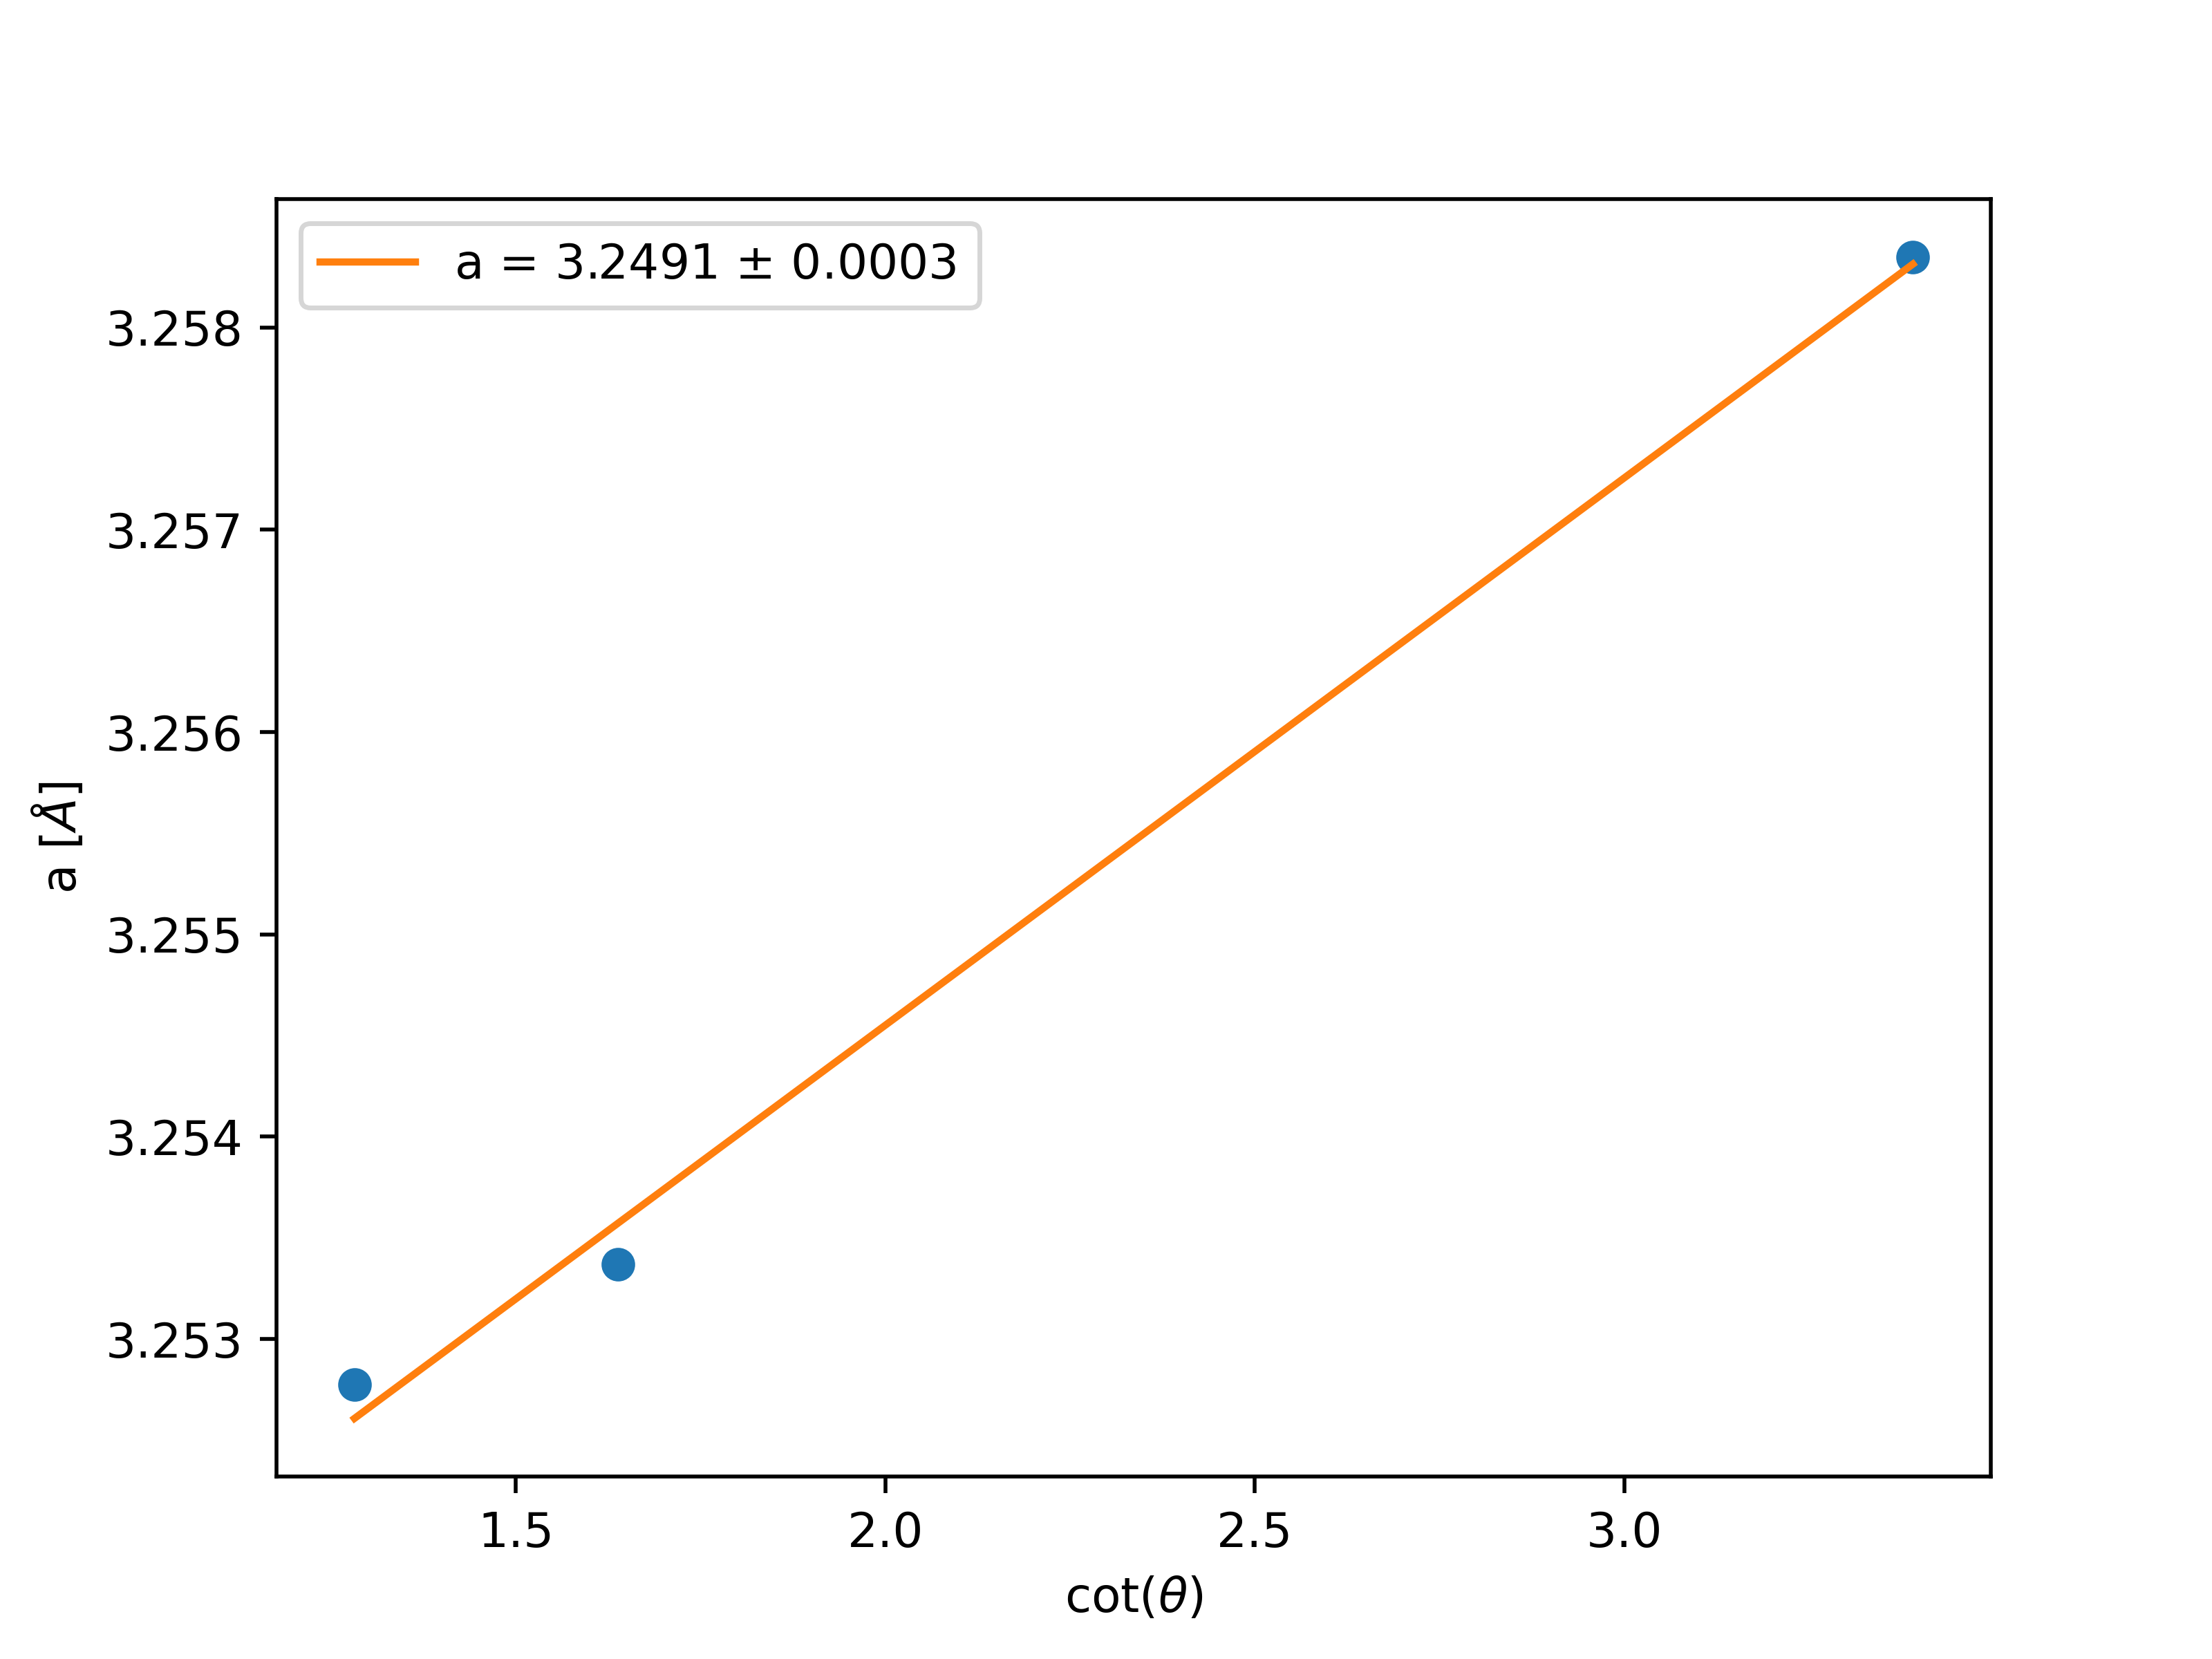
\includegraphics[width=\textwidth]{Figures/ZnOCotA.png}
		\caption{Fit 2: $a=3.2491 \pm \SI{0.0083}{\angstrom} $}
		\label{fig:ZnOFit2}
	\end{subfigure}
	\hfill
	\begin {subfigure}{0.3\textwidth}
		\centering
		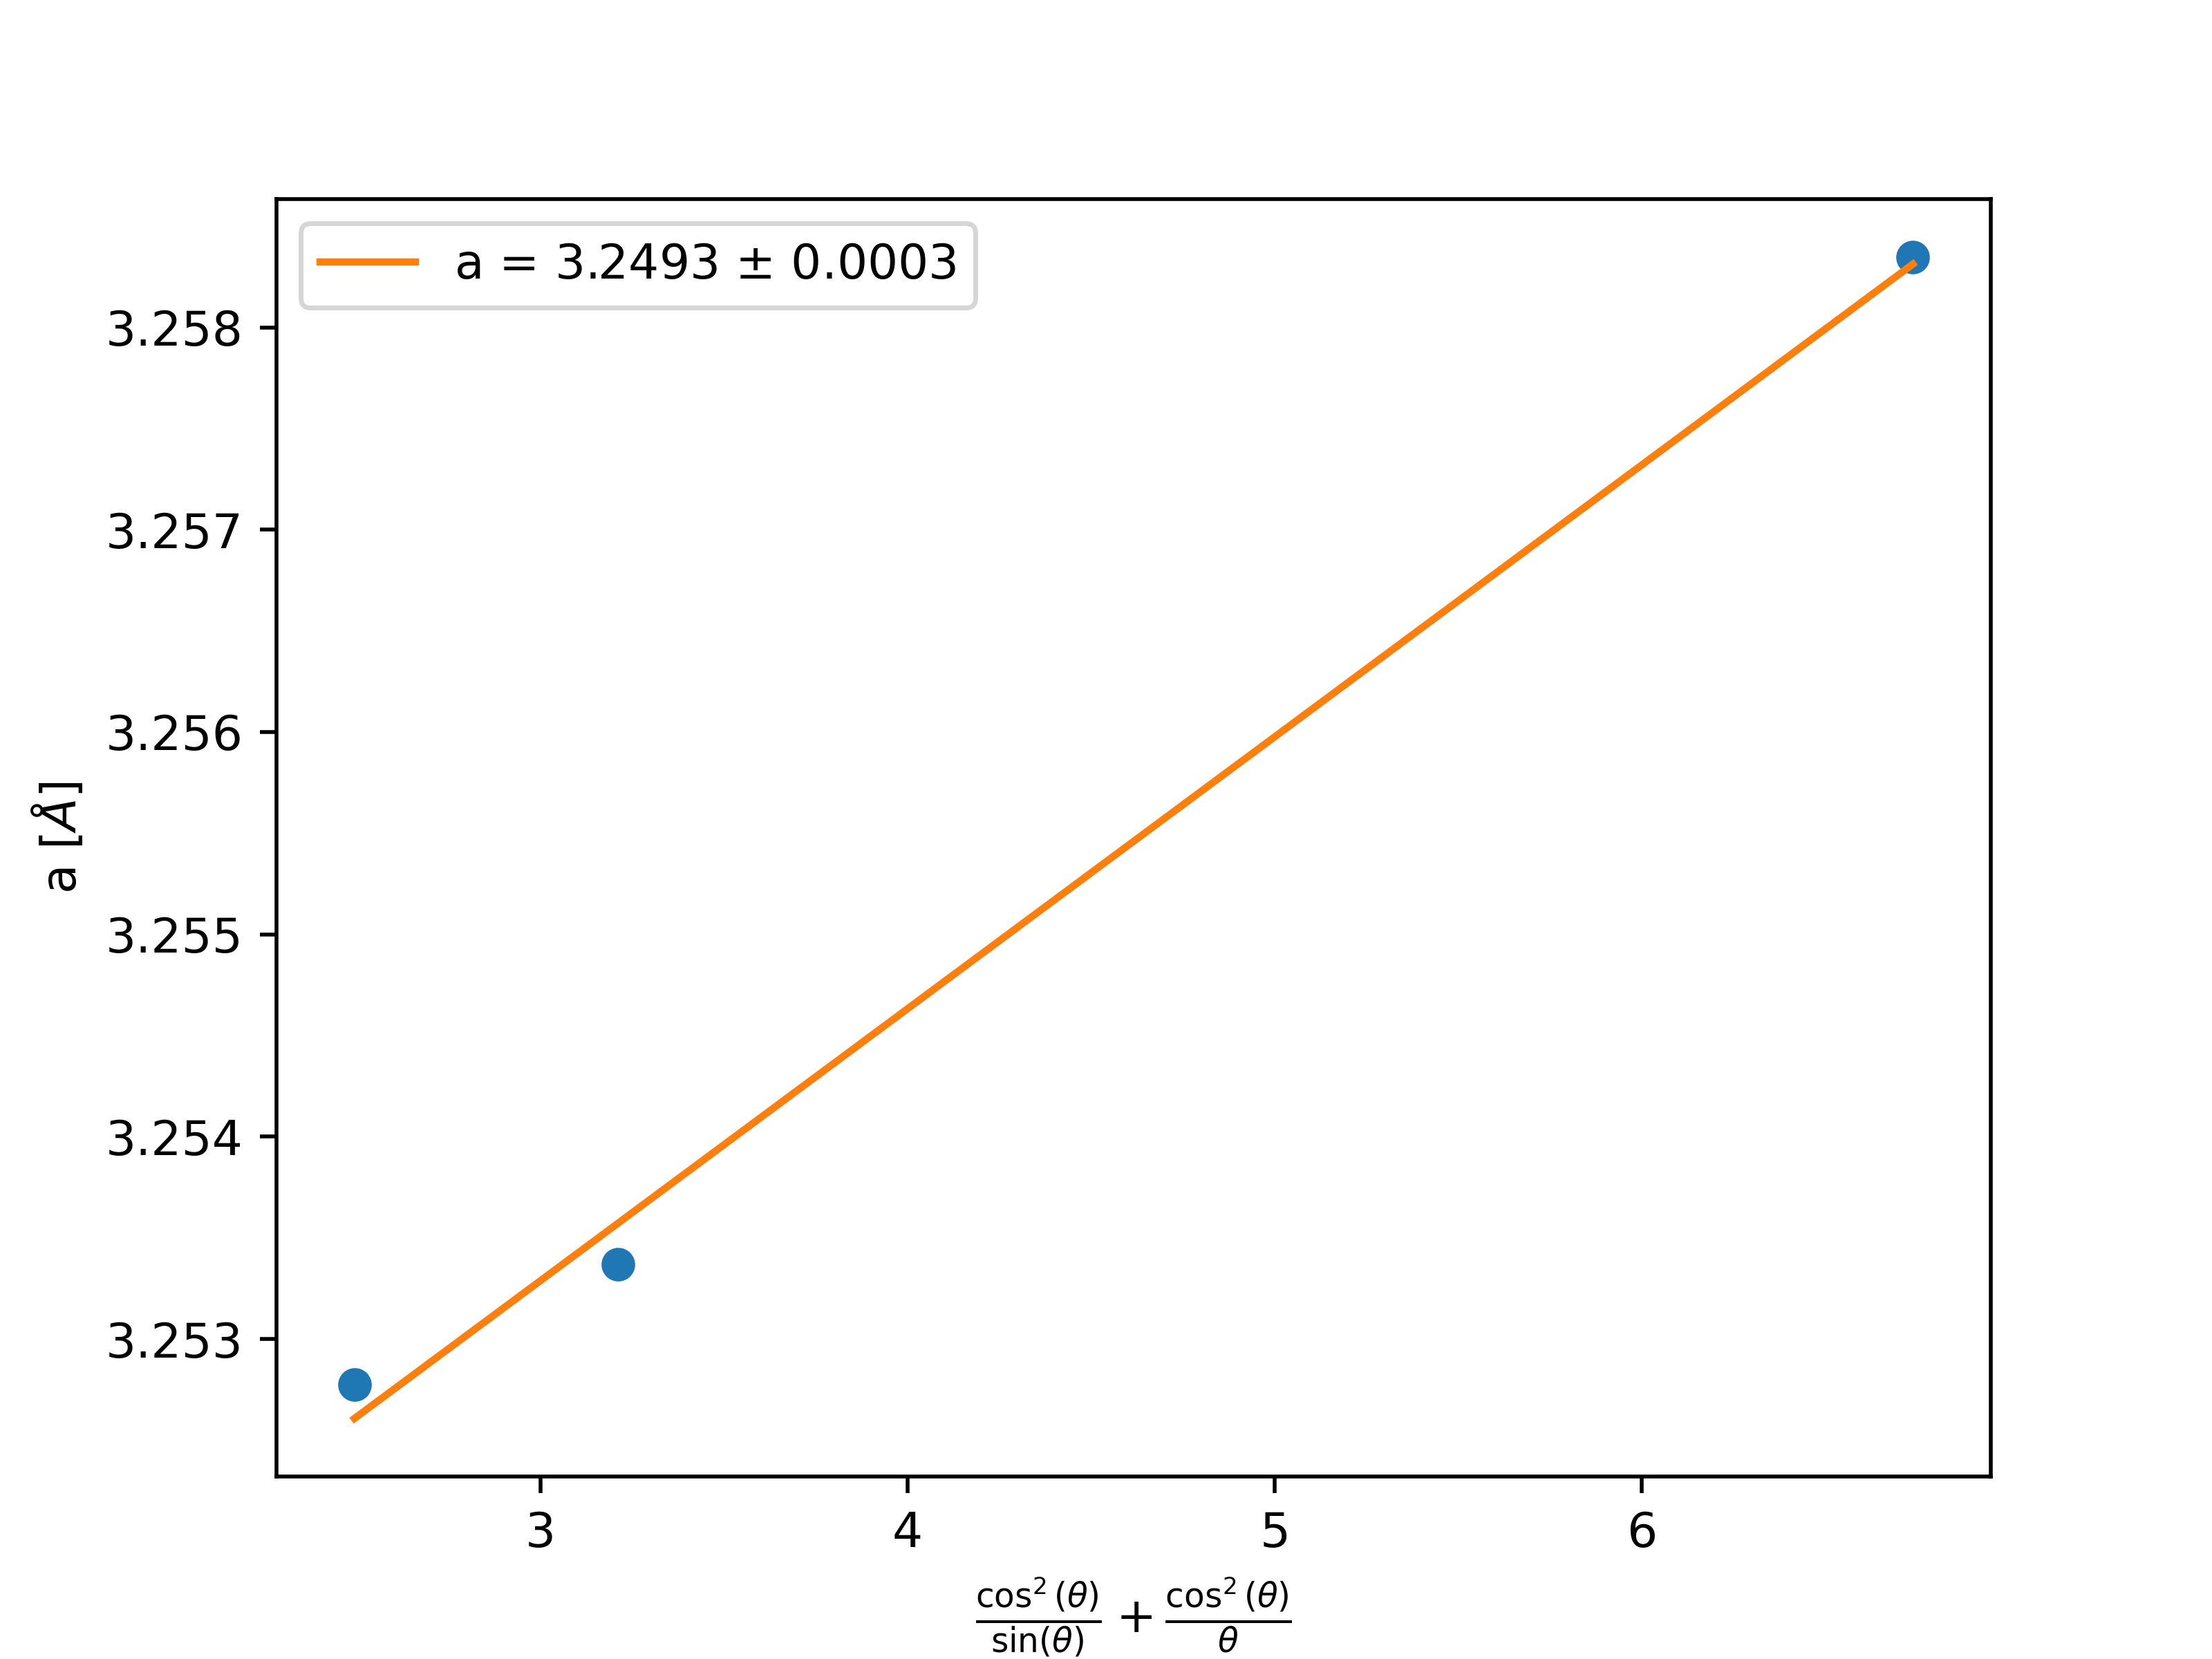
\includegraphics[width=\textwidth]{Figures/ZnONelsonA.png}
		\caption{Fit 3: $a=3.2493 \pm \SI{0.0003}{\angstrom} $}
		\label{fig:ZnOFit3}
	\end{subfigure}
	\begin {subfigure}{0.3\textwidth}
		\centering
		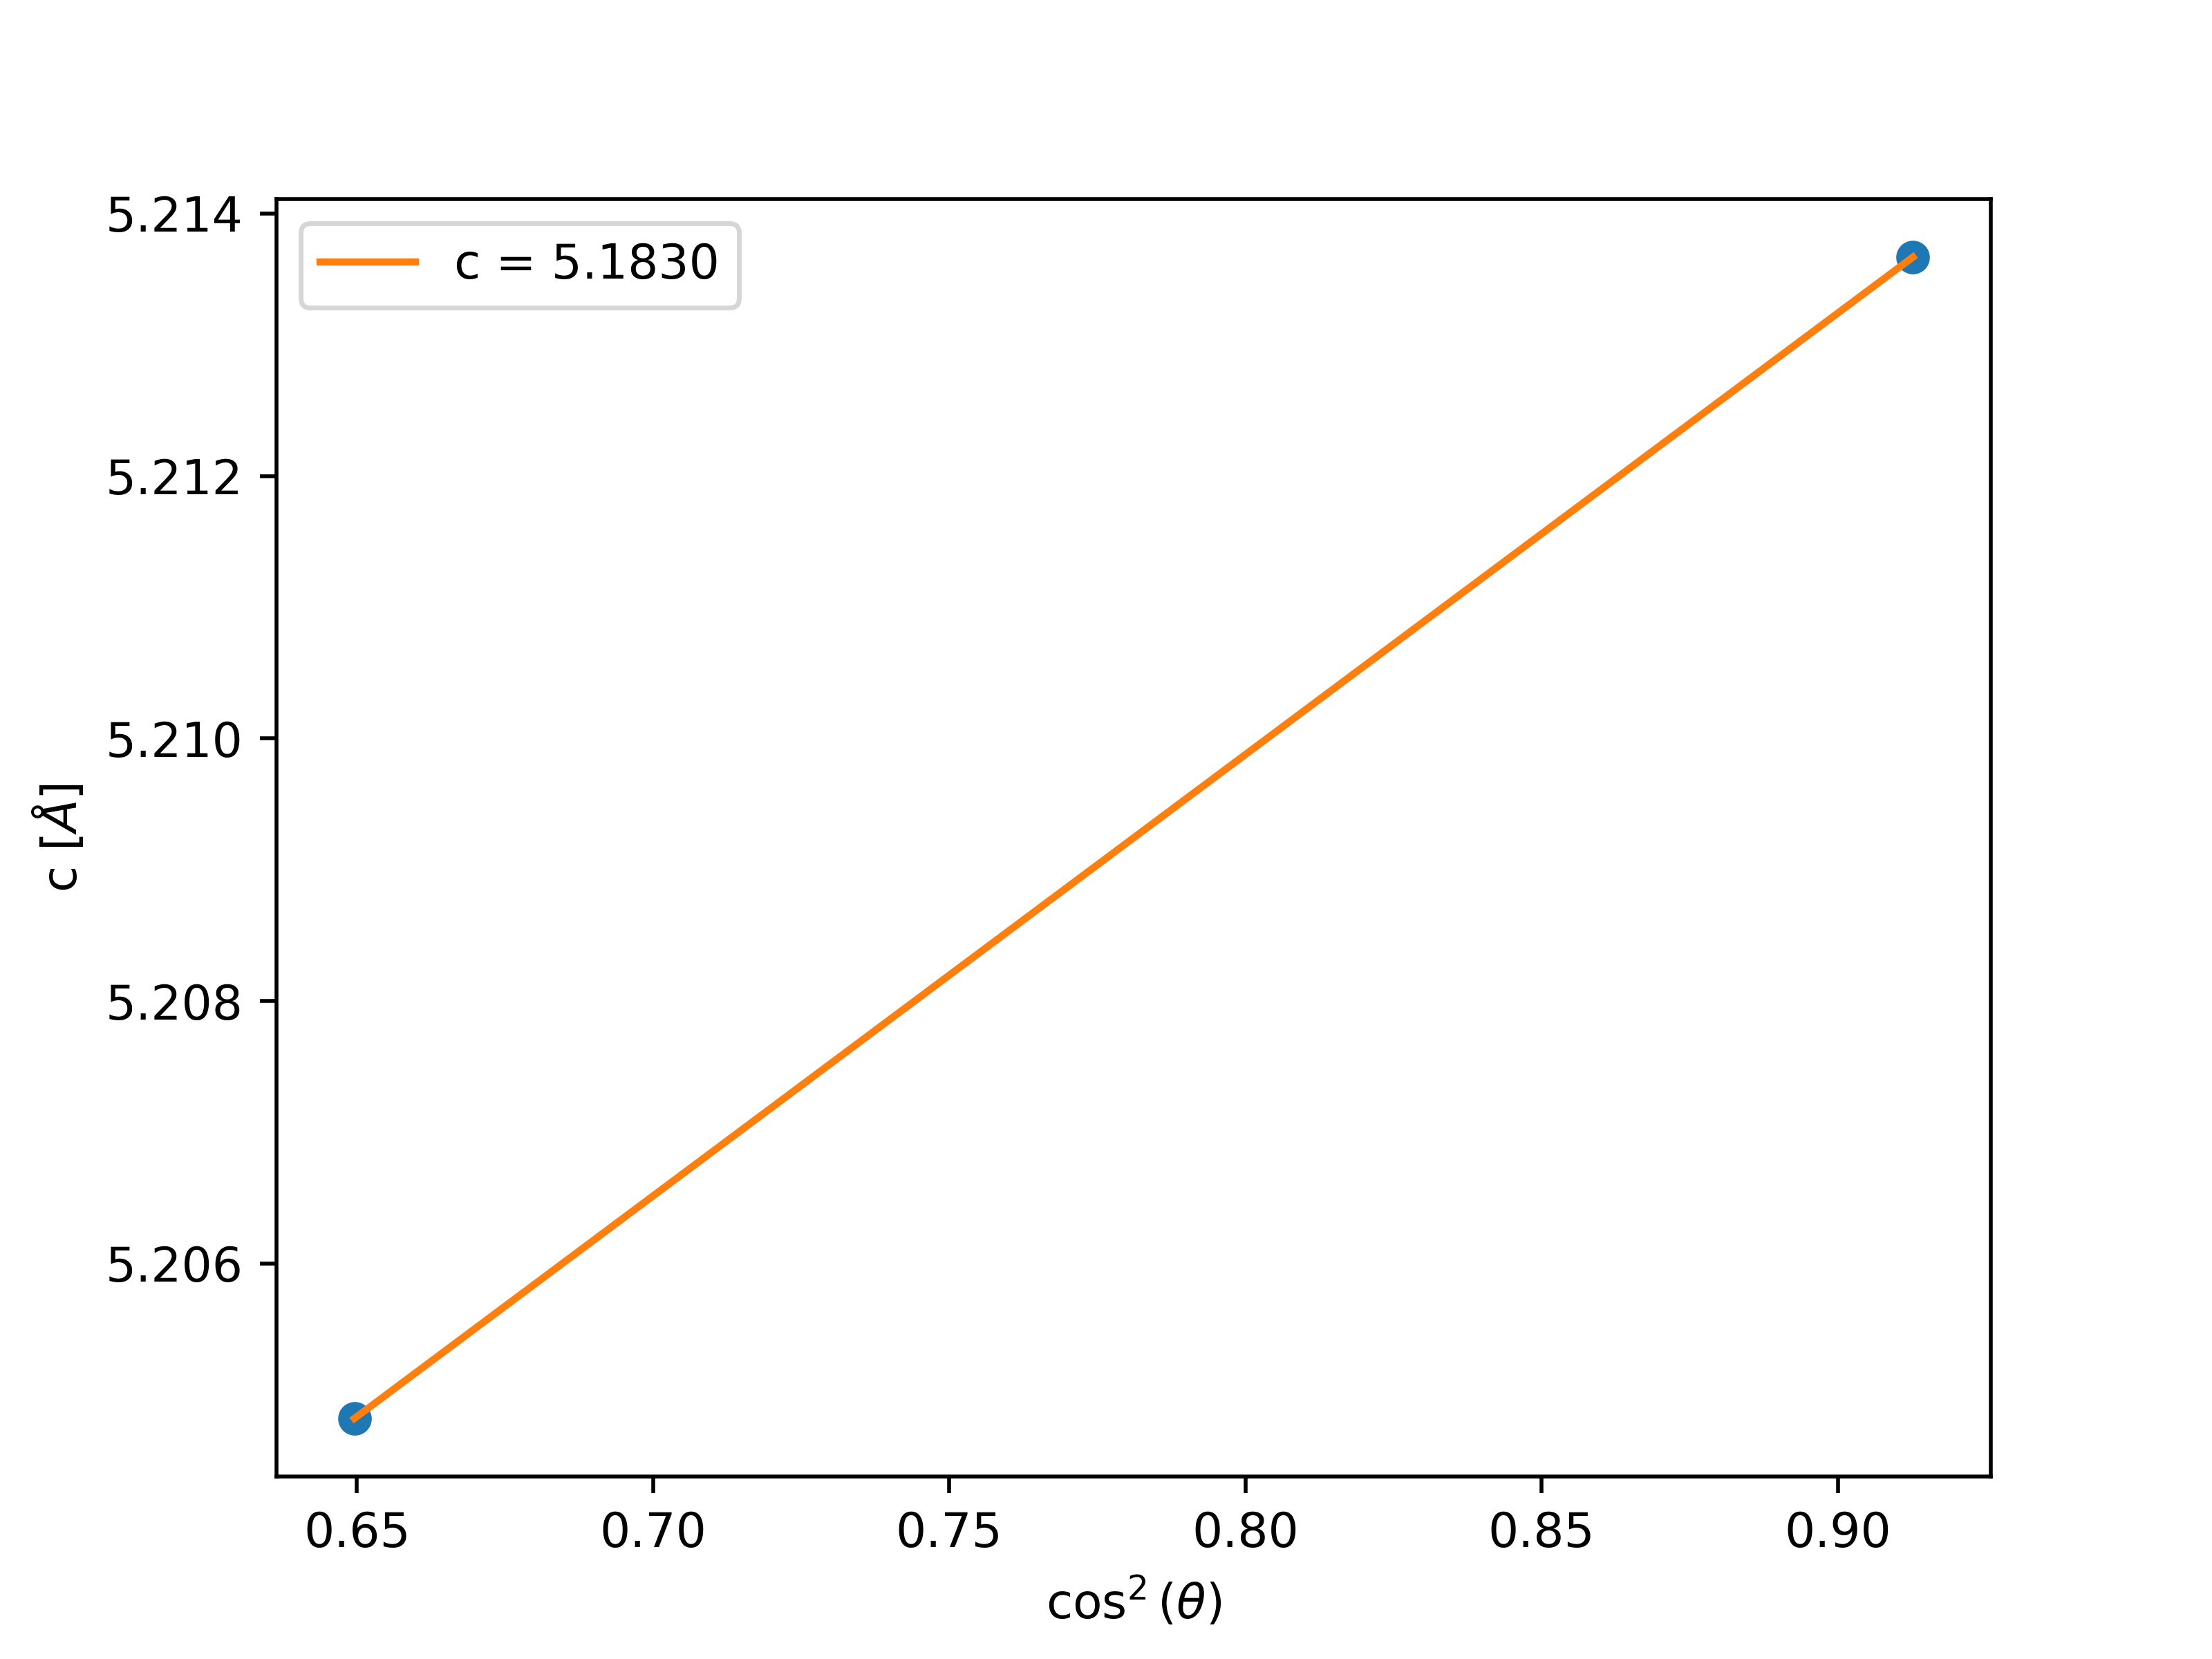
\includegraphics[width=\textwidth]{Figures/ZnOCosC.png}
		\caption{Fit 4: $c=\SI{5.1830}{\angstrom}$} 
		\label{fig:ZnOFit4}
	\end{subfigure}
	\hfill
	\begin {subfigure}{0.3\textwidth}
		\centering
		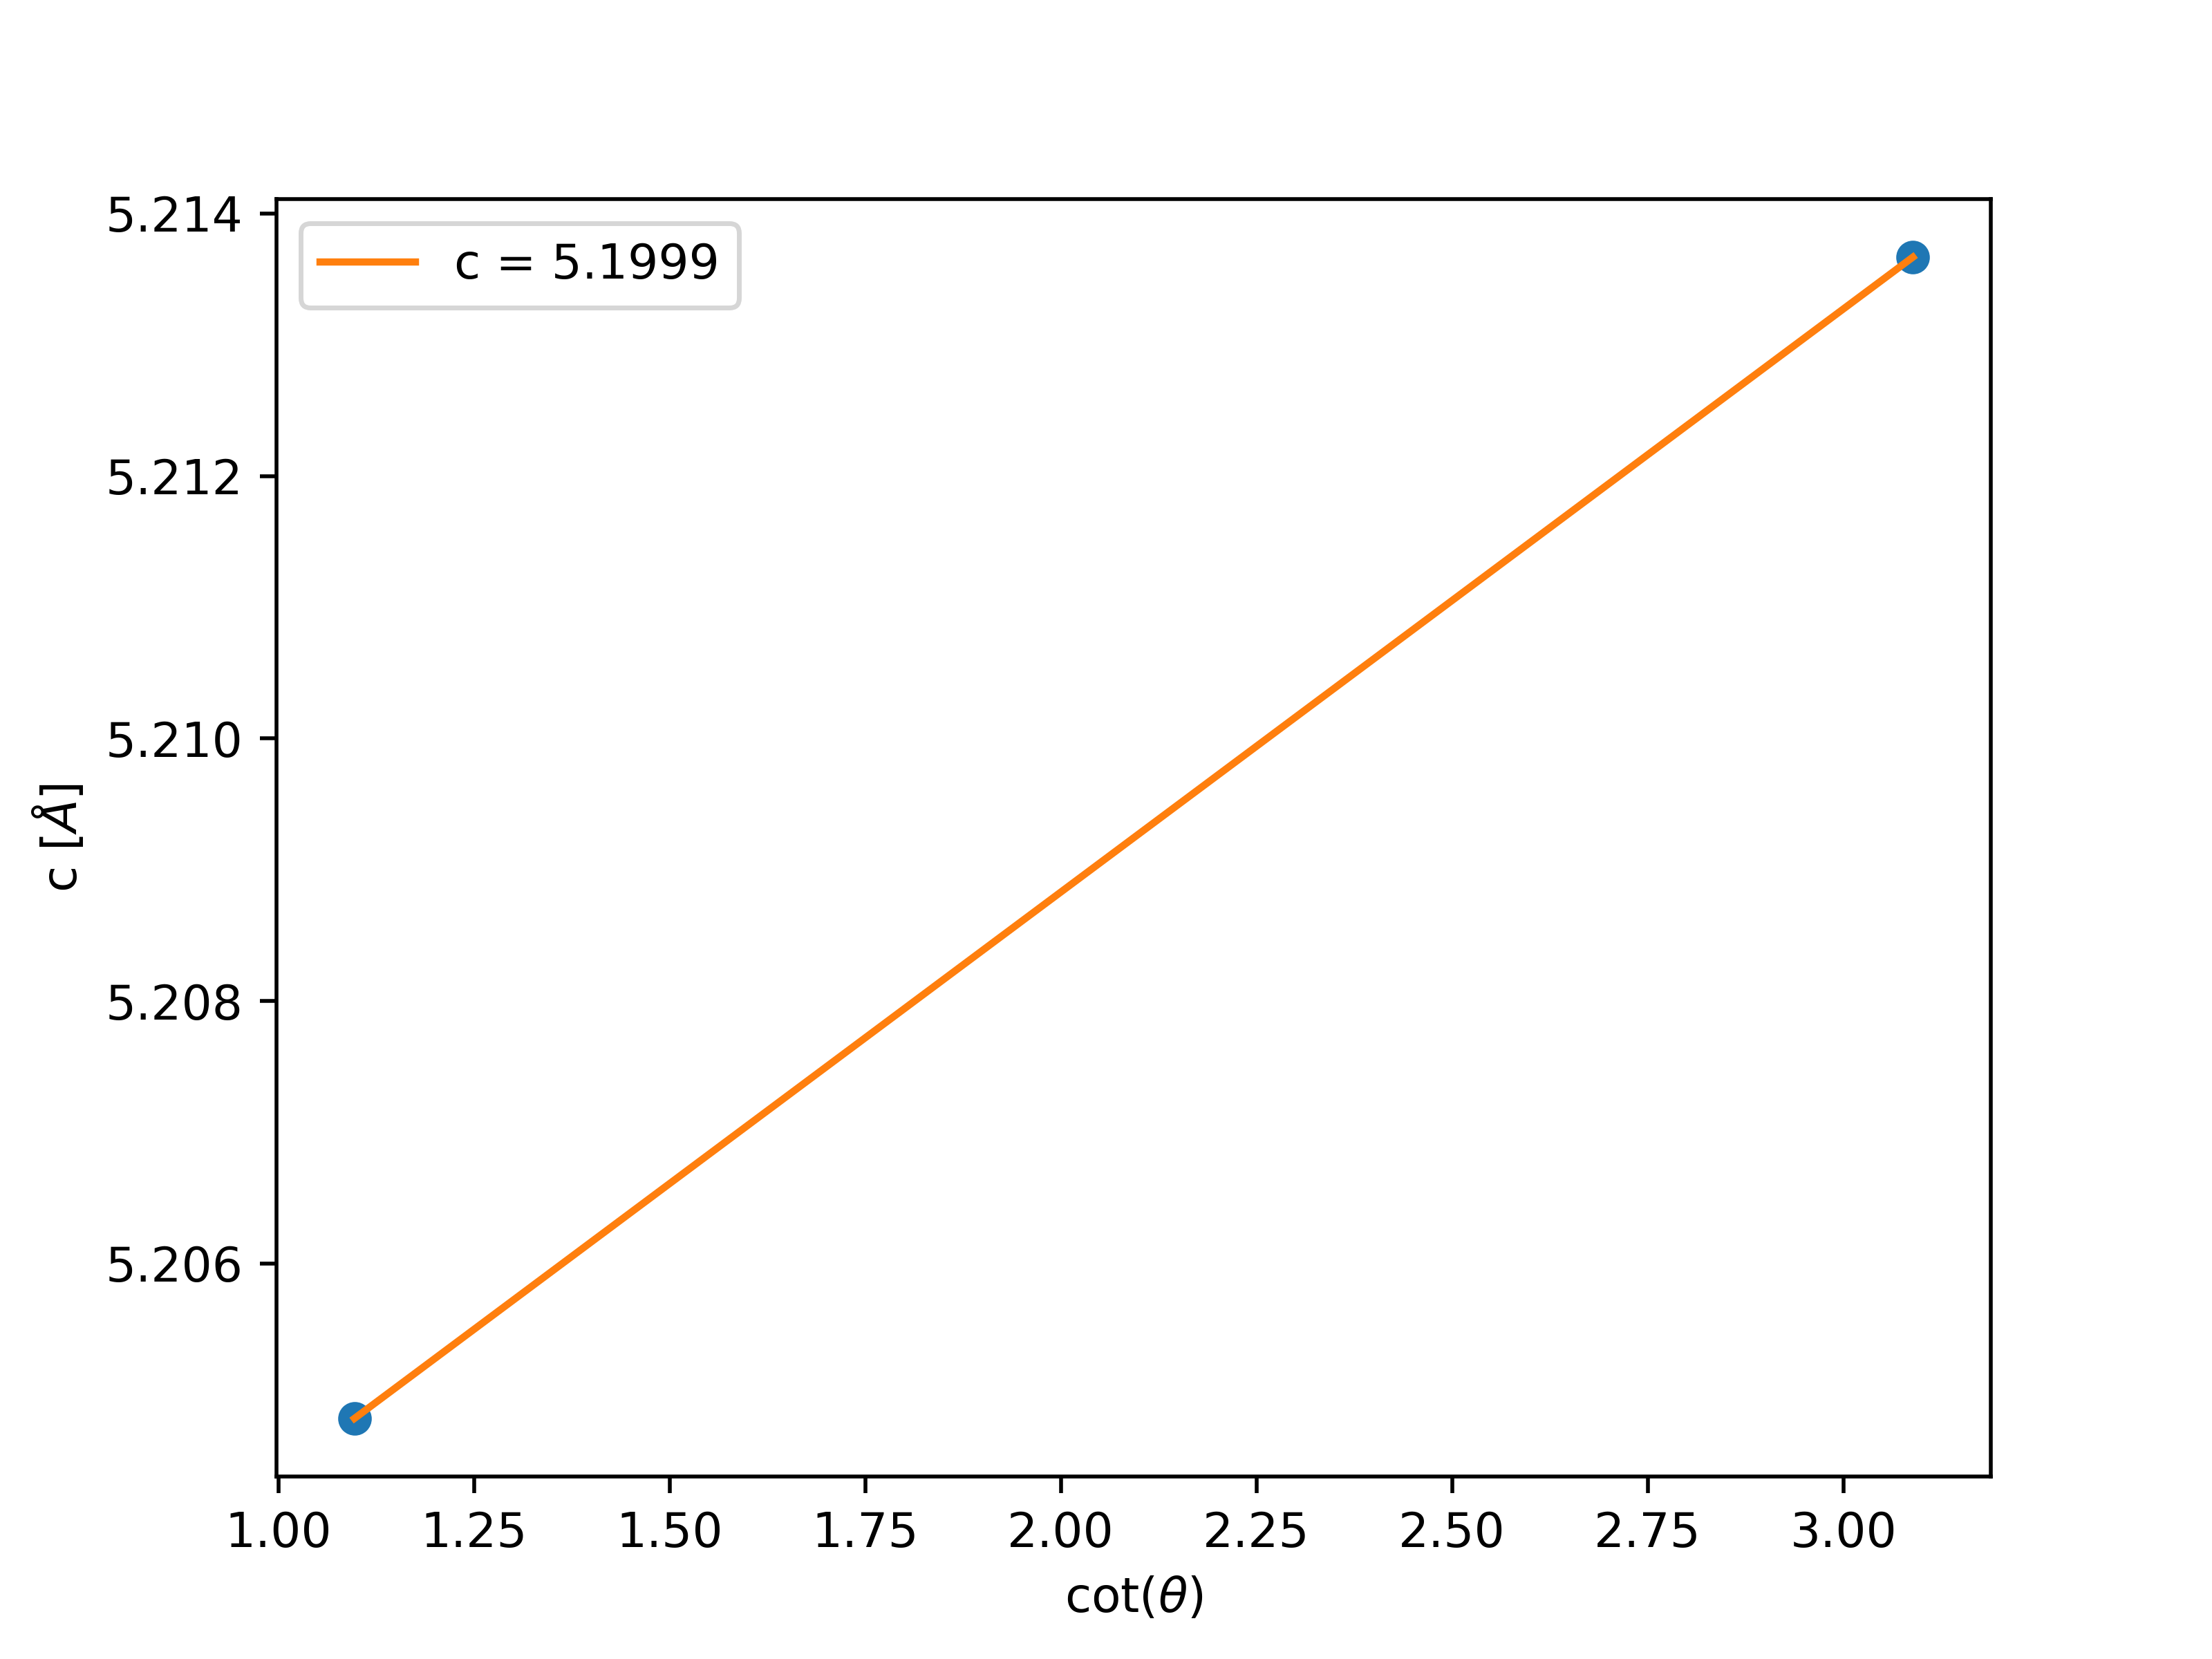
\includegraphics[width=\textwidth]{Figures/ZnOCotC.png}
		\caption{Fit 5: $c=\SI{5.1999}{\angstrom}$}
		\label{fig:ZnOFit5}
	\end{subfigure}
	\hfill
	\begin {subfigure}{0.3\textwidth}
		\centering
		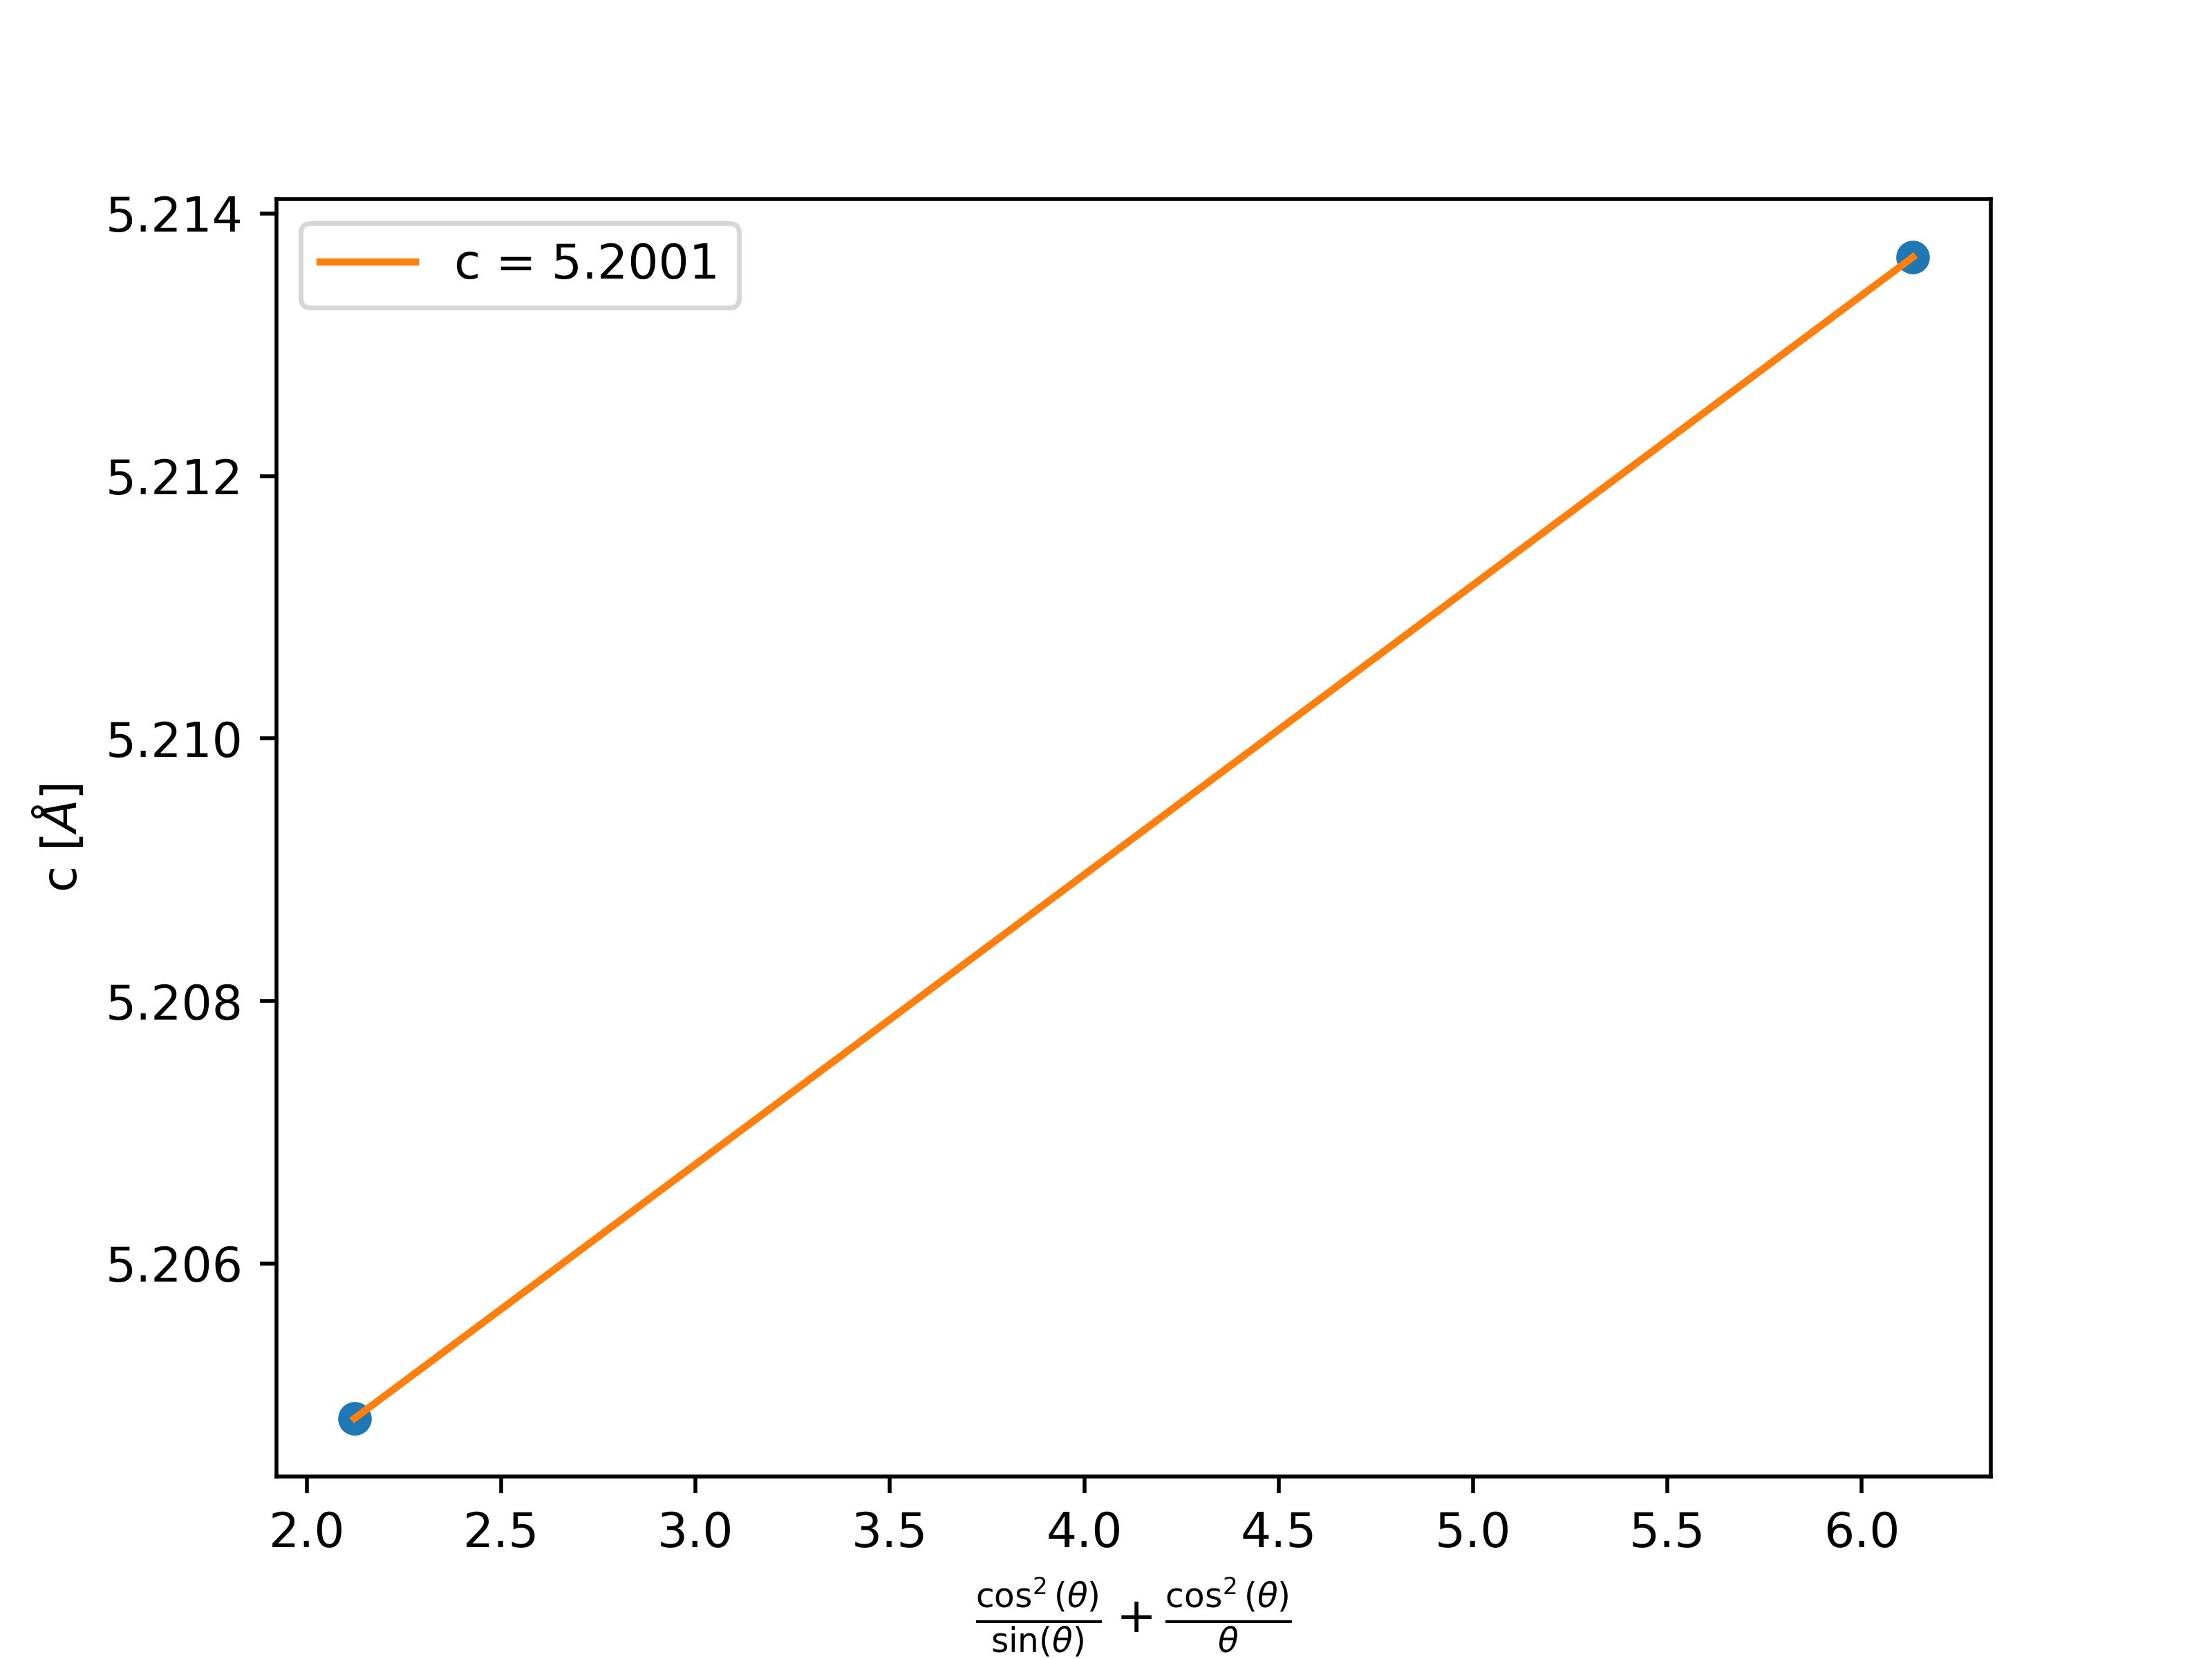
\includegraphics[width=\textwidth]{Figures/ZnONelsonC.png}
		\caption{Fit 6: $c=\SI{5.2001}{\angstrom}$}
		\label{fig:ZnOFit6}
	\end{subfigure}
\caption{Fits for ZnO.}
\label{fig:ZnOFits}
\end{figure}

Once again, the third fit against the Nelson-Riley function was the best fit, with the lattice constant $a=\SI{3.2493}{\angstrom}$
being $~ 0.02 \%$ off from the PC-PDF value, and the lattice constant $c=\SI{5.2001}{\angstrom}$ being $~ 0.1 \%$ off from the PC-PDF value. 


	For sapphire, the fit used many points and had pretty low uncertainty, in addition to the lattice constant being quite close to the PC-PDF value.
For ZnO, the fit for the $a$ parameter used only 3 points while the fit for the $c$ parameter used 2. While 3 points is enough to make a line and find its intercept, its usually better to have more points for accuracy. However, our data did not allow for that. Furthermore, It does not make sense to a line against only 2 points, as one can draw any line between two points. This is why $c$ is noticably less accurate than $a$, and why it has no uncertainty. 
However, the report did specify to use a best fit line, and this is what was done. Maybe what should be done instead is a statistical analysis with an average and a standard deviation which might be more accurate.

\pagebreak{}

\subsection{Task 2}
\label{subsection:Task2}

\subsubsection{Spectral Lines}

	In this task we analyze the diffraction patterns generated by the $2\theta - \omega$ and $\omega$ scans of two ZnO thin films grown on a-plane and r-plane oriented sapphire substrates. We compare the results to the previous task where a powder sample was used. The peaks of the a-grown sapphire substrate and the corresponding sample are shown in the figures below. The lines marking the peaks are purple for Cu-K$\beta$, red for Cu-K$\alpha$1, green for Cu-K$\alpha$2 and blue for Tungsten. This peak assignment was done using the Spectral Lines tool in the Data Viewer software. 



\begin{figure}[h]
    \centering
    \begin{subfigure}[b]{0.45\textwidth}
        \centering
        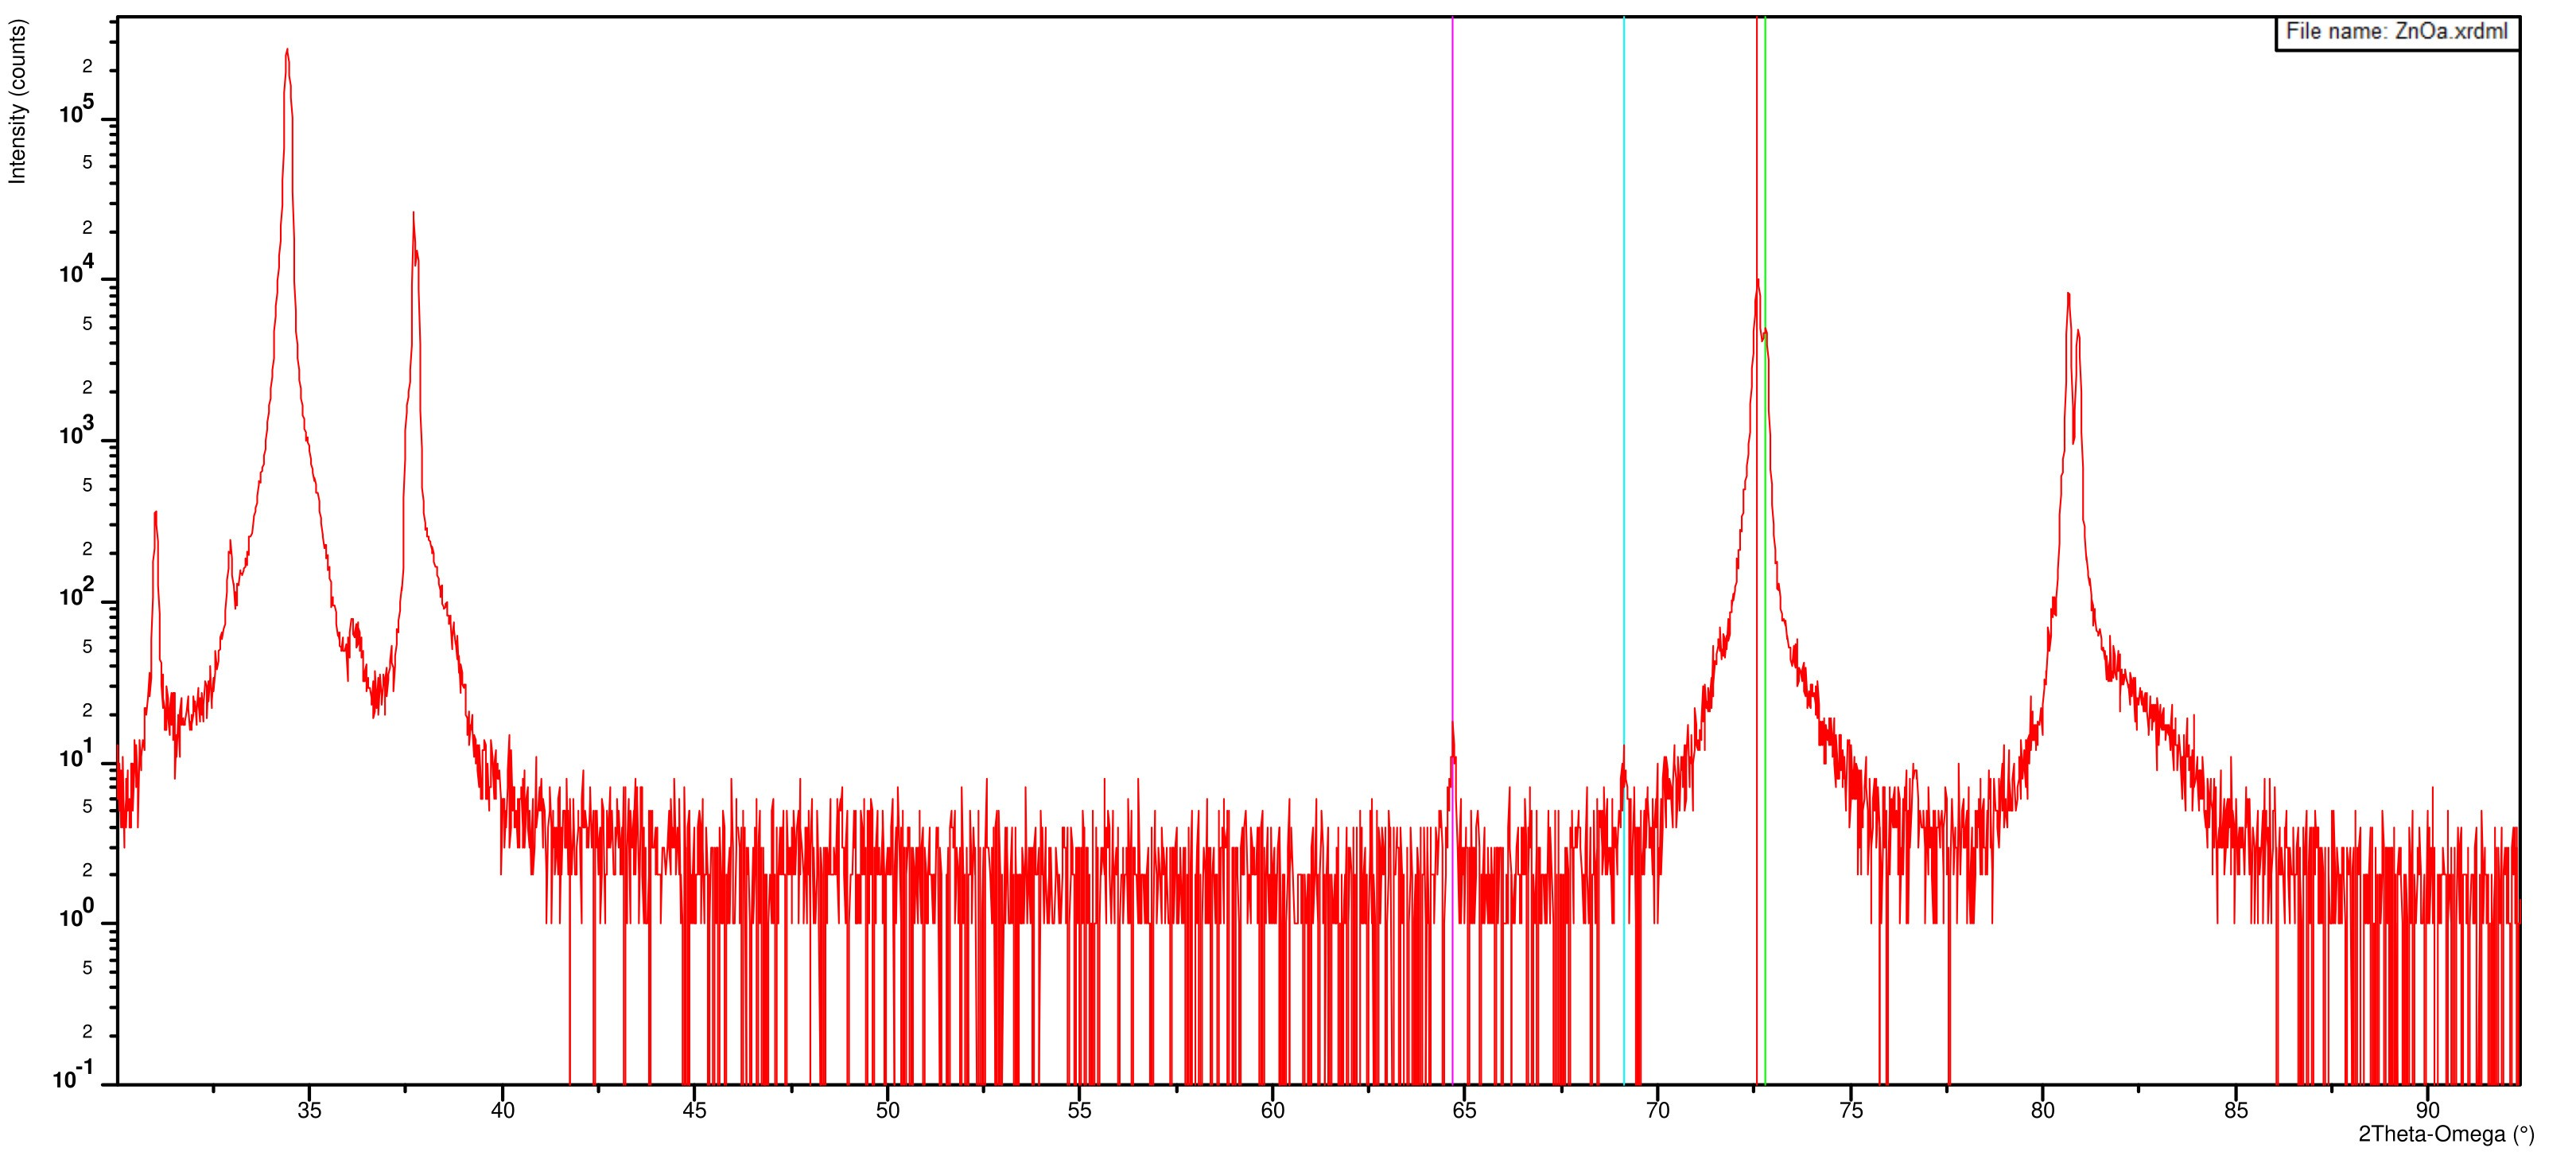
\includegraphics[width=\textwidth]{Figures/a-plane-sapphire-peaks.jpg} % Replace with your image file
        \caption{a-plane sapphire peaks}
        \label{fig:subfig1}
    \end{subfigure}
    \hfill
    \begin{subfigure}[b]{0.45\textwidth}
        \centering
        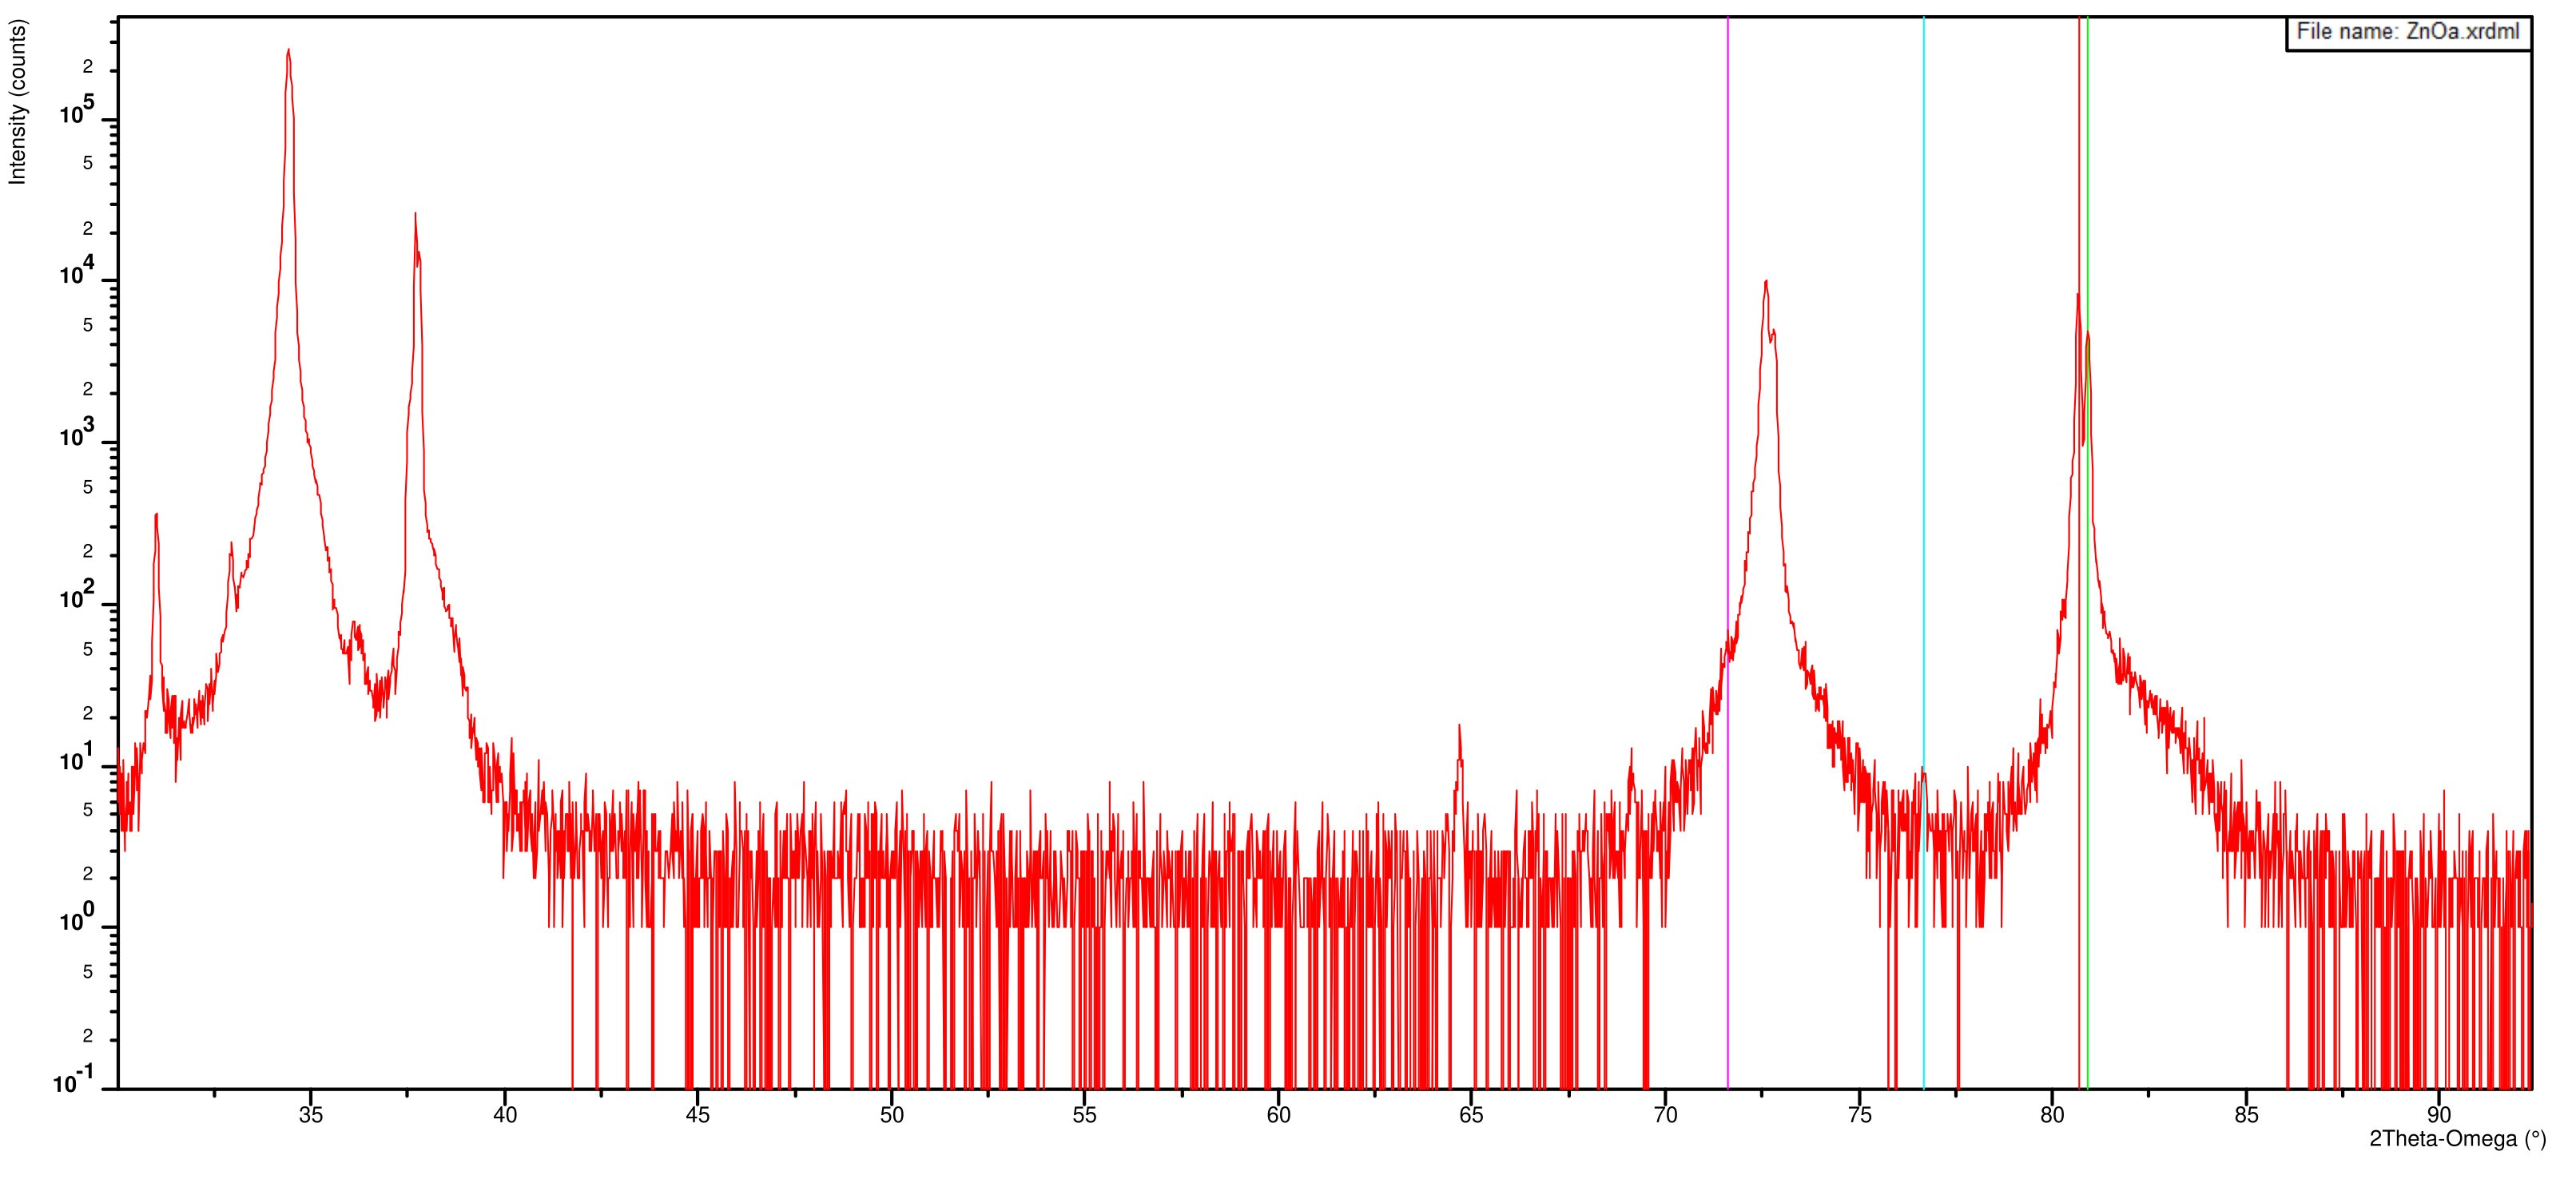
\includegraphics[width=\textwidth]{Figures/a-plane-ZnO-peaks.jpg} % Replace with your image file
        \caption{a-plane ZnO peaks}
        \label{fig:subfig2}
    \end{subfigure}
    
    \vspace{1em} % Add some vertical space between the rows

    \begin{subfigure}[b]{0.45\textwidth}
        \centering
        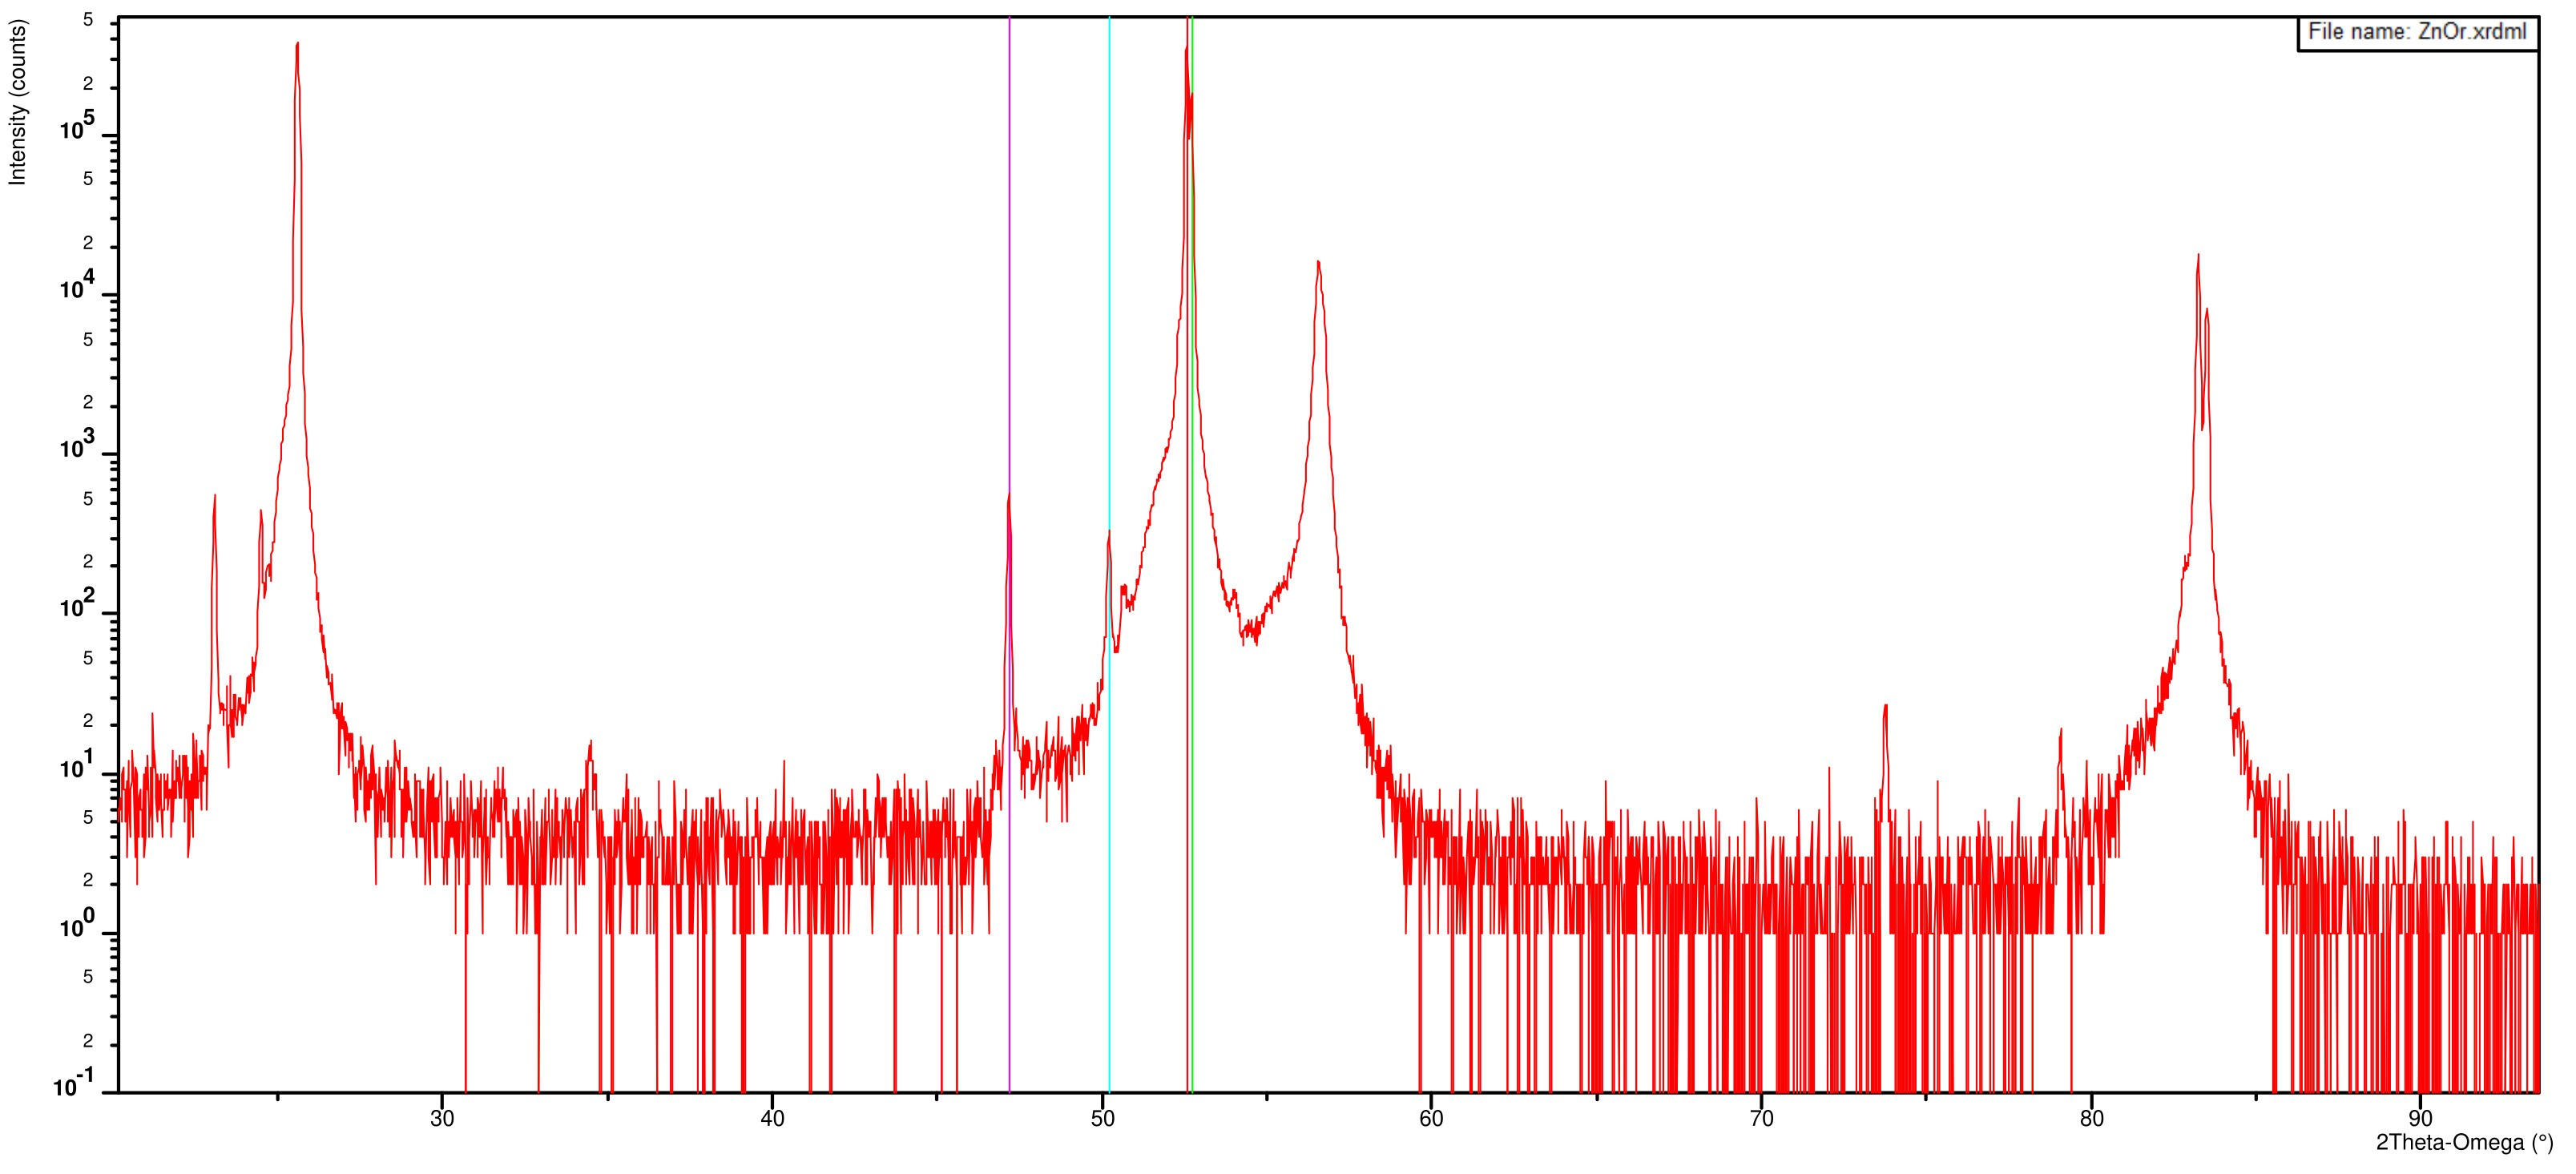
\includegraphics[width=\textwidth]{Figures/r-plane-sapphire-peaks.jpg} % Replace with your image file
        \caption{r-plane sapphire peaks}
        \label{fig:subfig3}
    \end{subfigure}
    \hfill
    \begin{subfigure}[b]{0.45\textwidth}
        \centering
        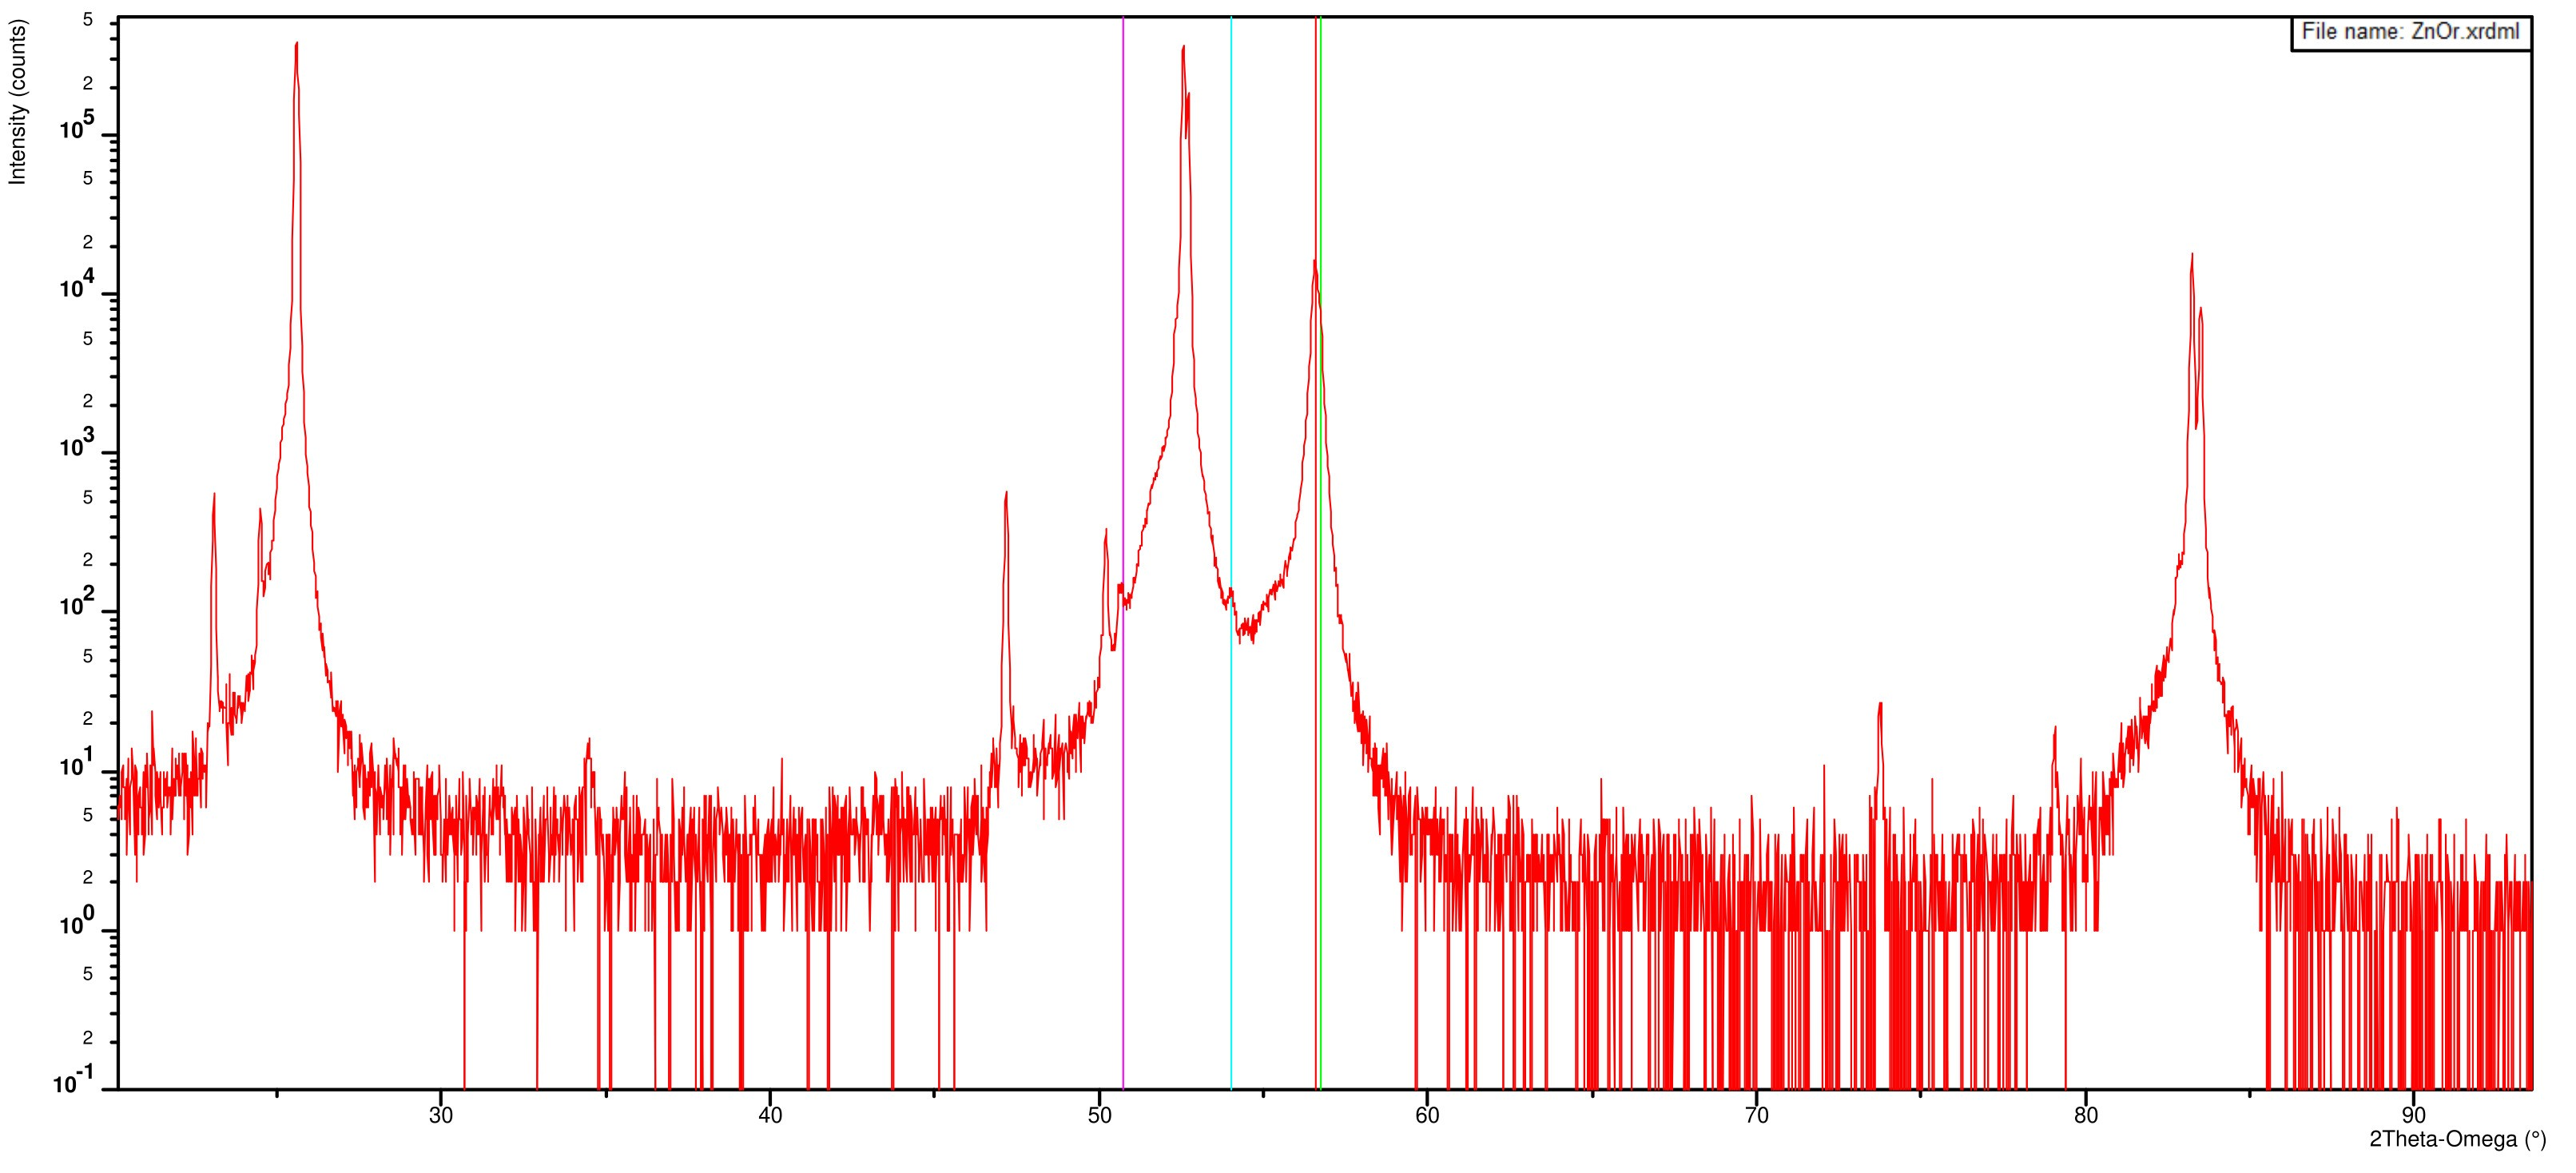
\includegraphics[width=\textwidth]{Figures/r-plane-ZnO-peaks.jpg} % Replace with your image file
        \caption{r-plane ZnO peaks}
        \label{fig:subfig4}
    \end{subfigure}

    \caption{Peaks of diffraction patterns from the $2\theta - \omega$ scans of the ZnO thin film}
    \label{fig:grouped}
\end{figure}

For powder samples more peaks show up since the grains have random orientations. In the $2\theta - \omega$ scans, we only observe peaks that correspond to crystallographic planes parallel to the surface of the sample (Thin films have specific orientations). This can be seen when comparing to Figure [\ref{fig:BraggPeaks}]. The thin film peaks are more intense because there is no destructive interference between different indices, since diffraction happens due to the same set of planes. We also notice a broadening of the peaks in the powder sample compared to the thin film sample. 


	We can find the crystallographic growth direction of the thin films using the Miller indices of the ZnO peaks. The peaks we observe for the thin film have miller indices of the form (00l) in the a-plane sapphire case. Hence, the film grows in the [0001] direction. Similarly, the r-plane sapphire thin film growth direction is [1100].
\pagebreak{}
\subsubsection{Rocking curves}
An $\omega$ scan is performed for the peak with the highest $2\theta$ value for both the substrate and the thin film. The FWHM of the rocking curves is determined. The following curevs were obtained: 

\begin{figure}[h]
    \centering
    \begin{subfigure}[b]{0.45\textwidth}
        \centering
        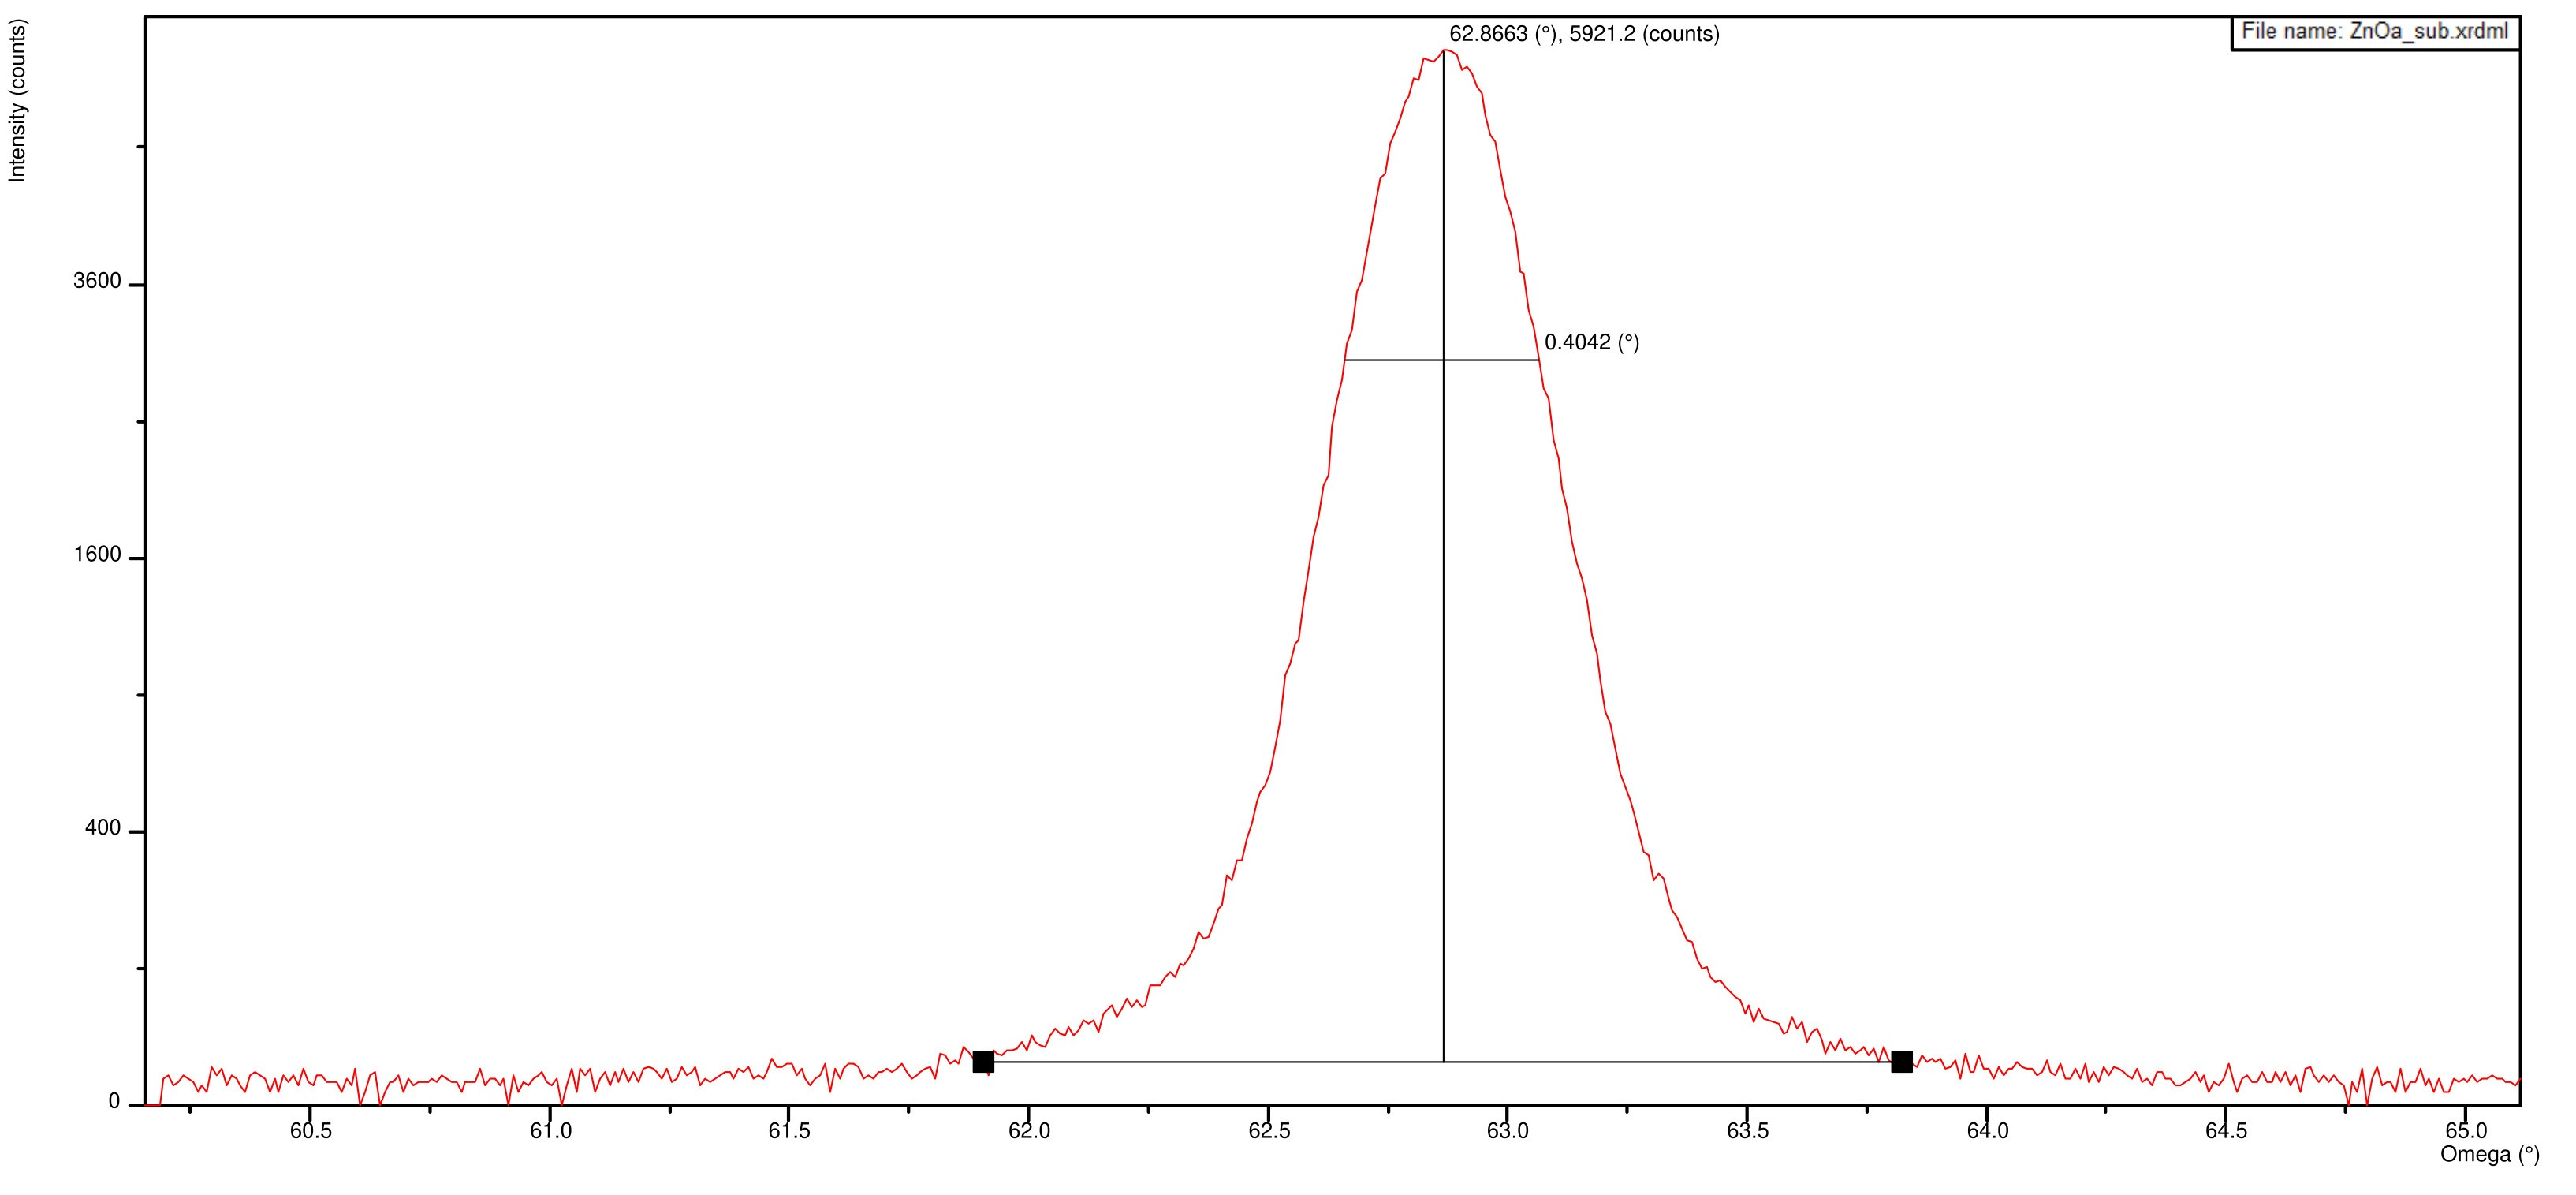
\includegraphics[width=\textwidth]{Figures/w-scan-a-plane-sapphire-peaks.jpg} % Replace with your image file
        \caption{a-plane ZnO peak}
        \label{fig:subfig1}
    \end{subfigure}
    \hfill
    \begin{subfigure}[b]{0.45\textwidth}
        \centering
        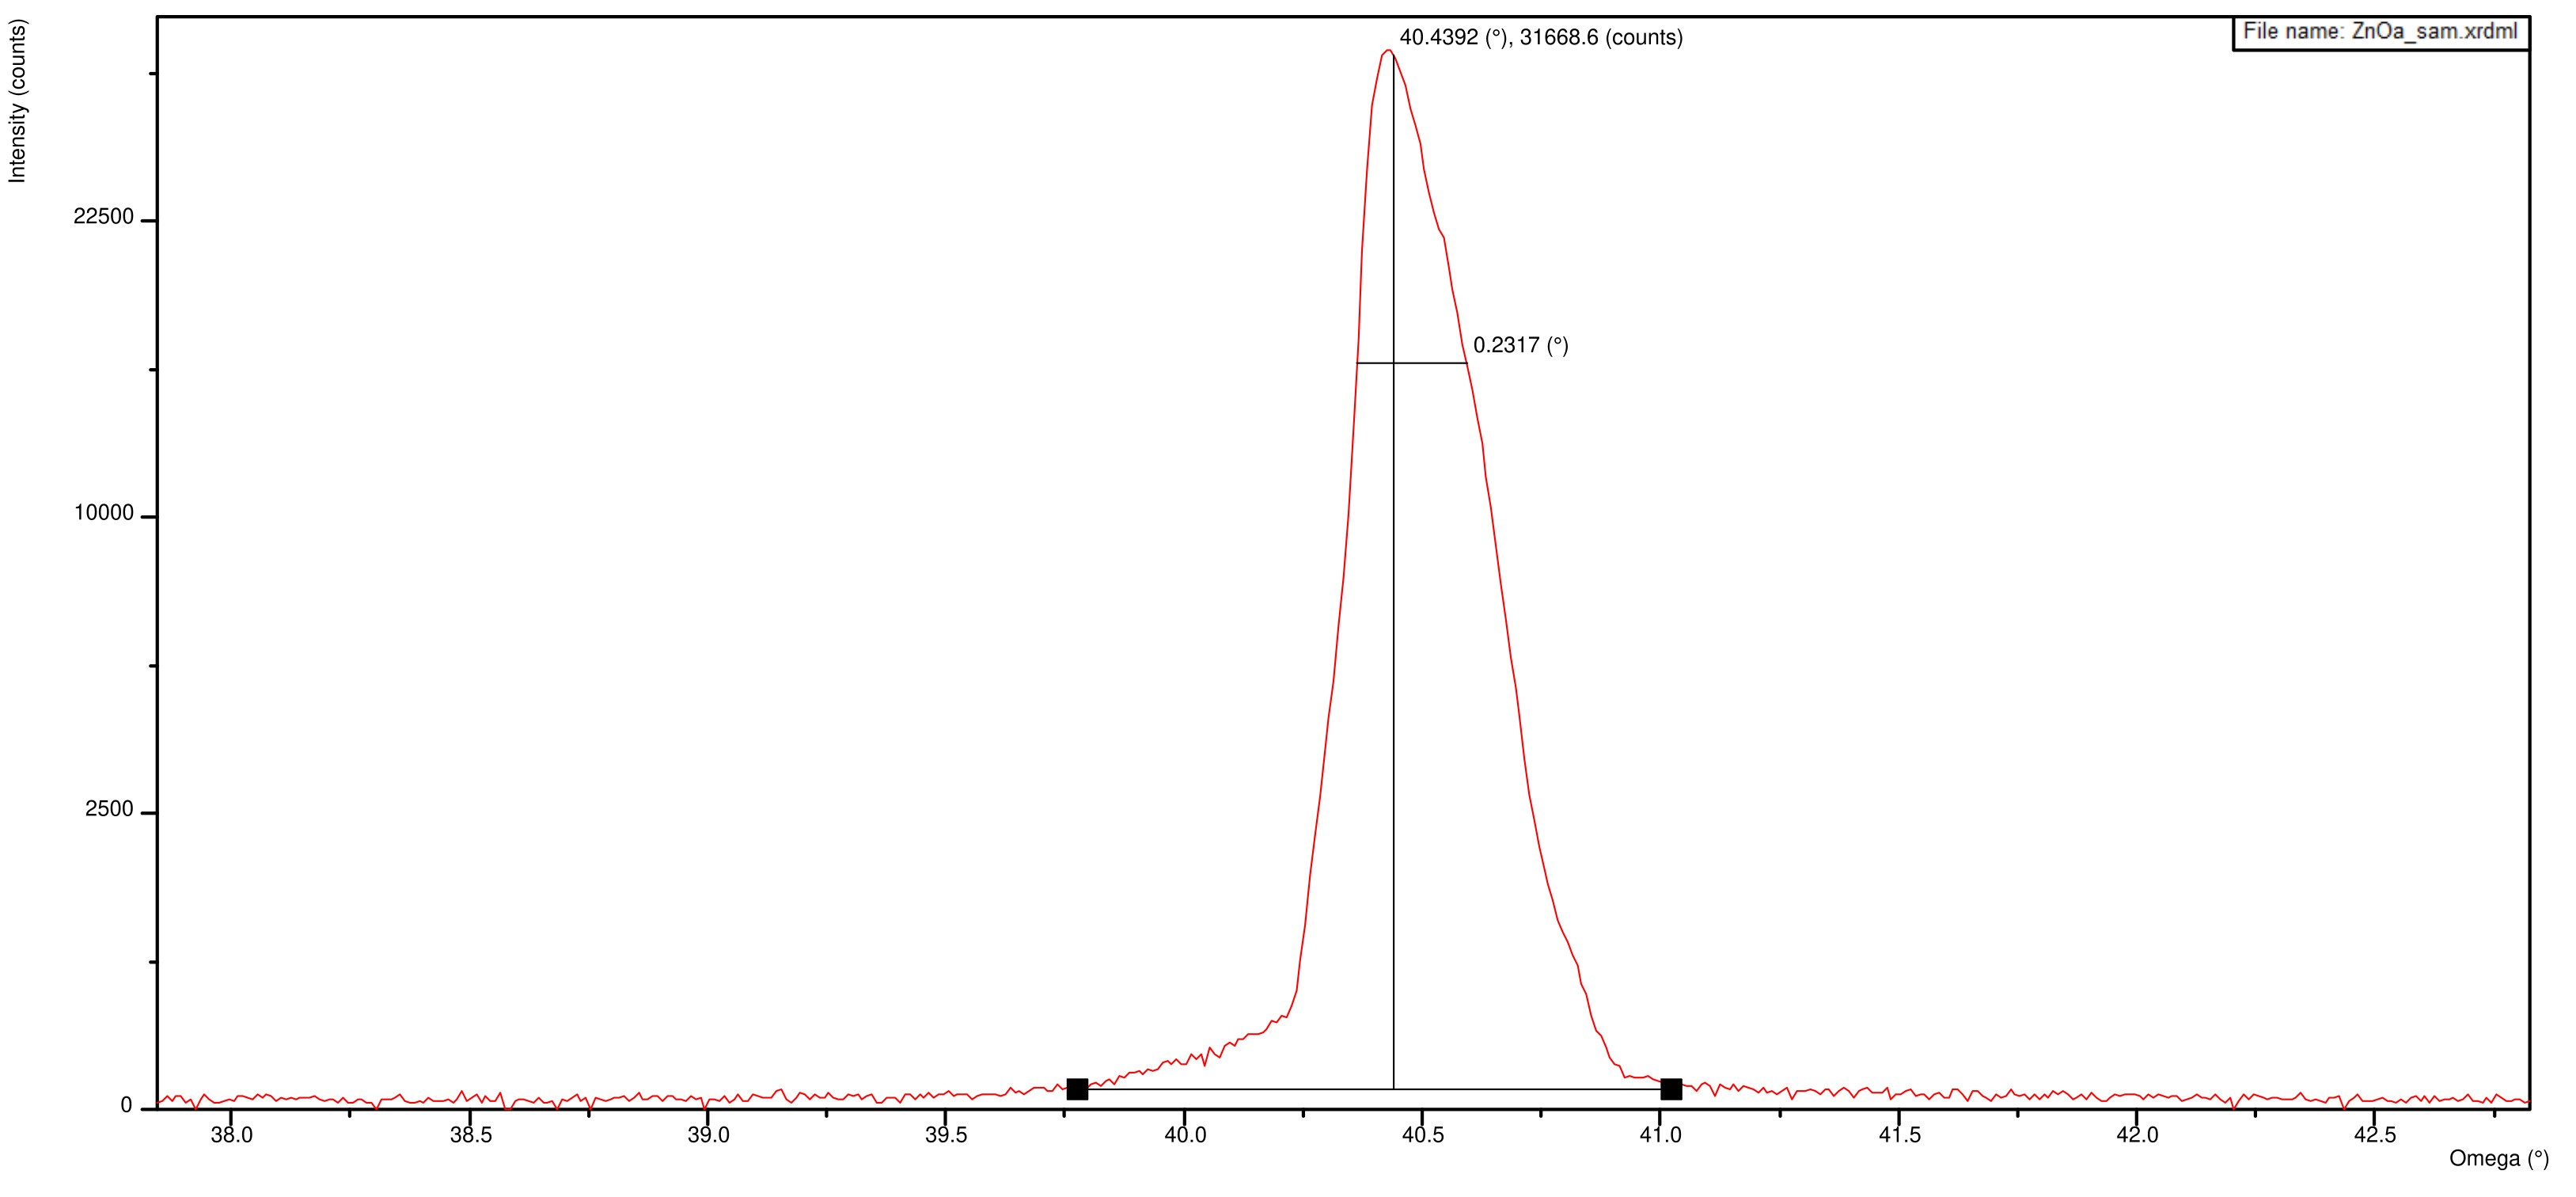
\includegraphics[width=\textwidth]{Figures/w-scan-ZnO-on-a-plane-sapphire-peaks.jpg} % Replace with your image file
        \caption{a-plane sapphire peak}
        \label{fig:subfig2}
    \end{subfigure}
    
    \vspace{1em} % Add some vertical space between the rows

    \begin{subfigure}[b]{0.45\textwidth}
        \centering
        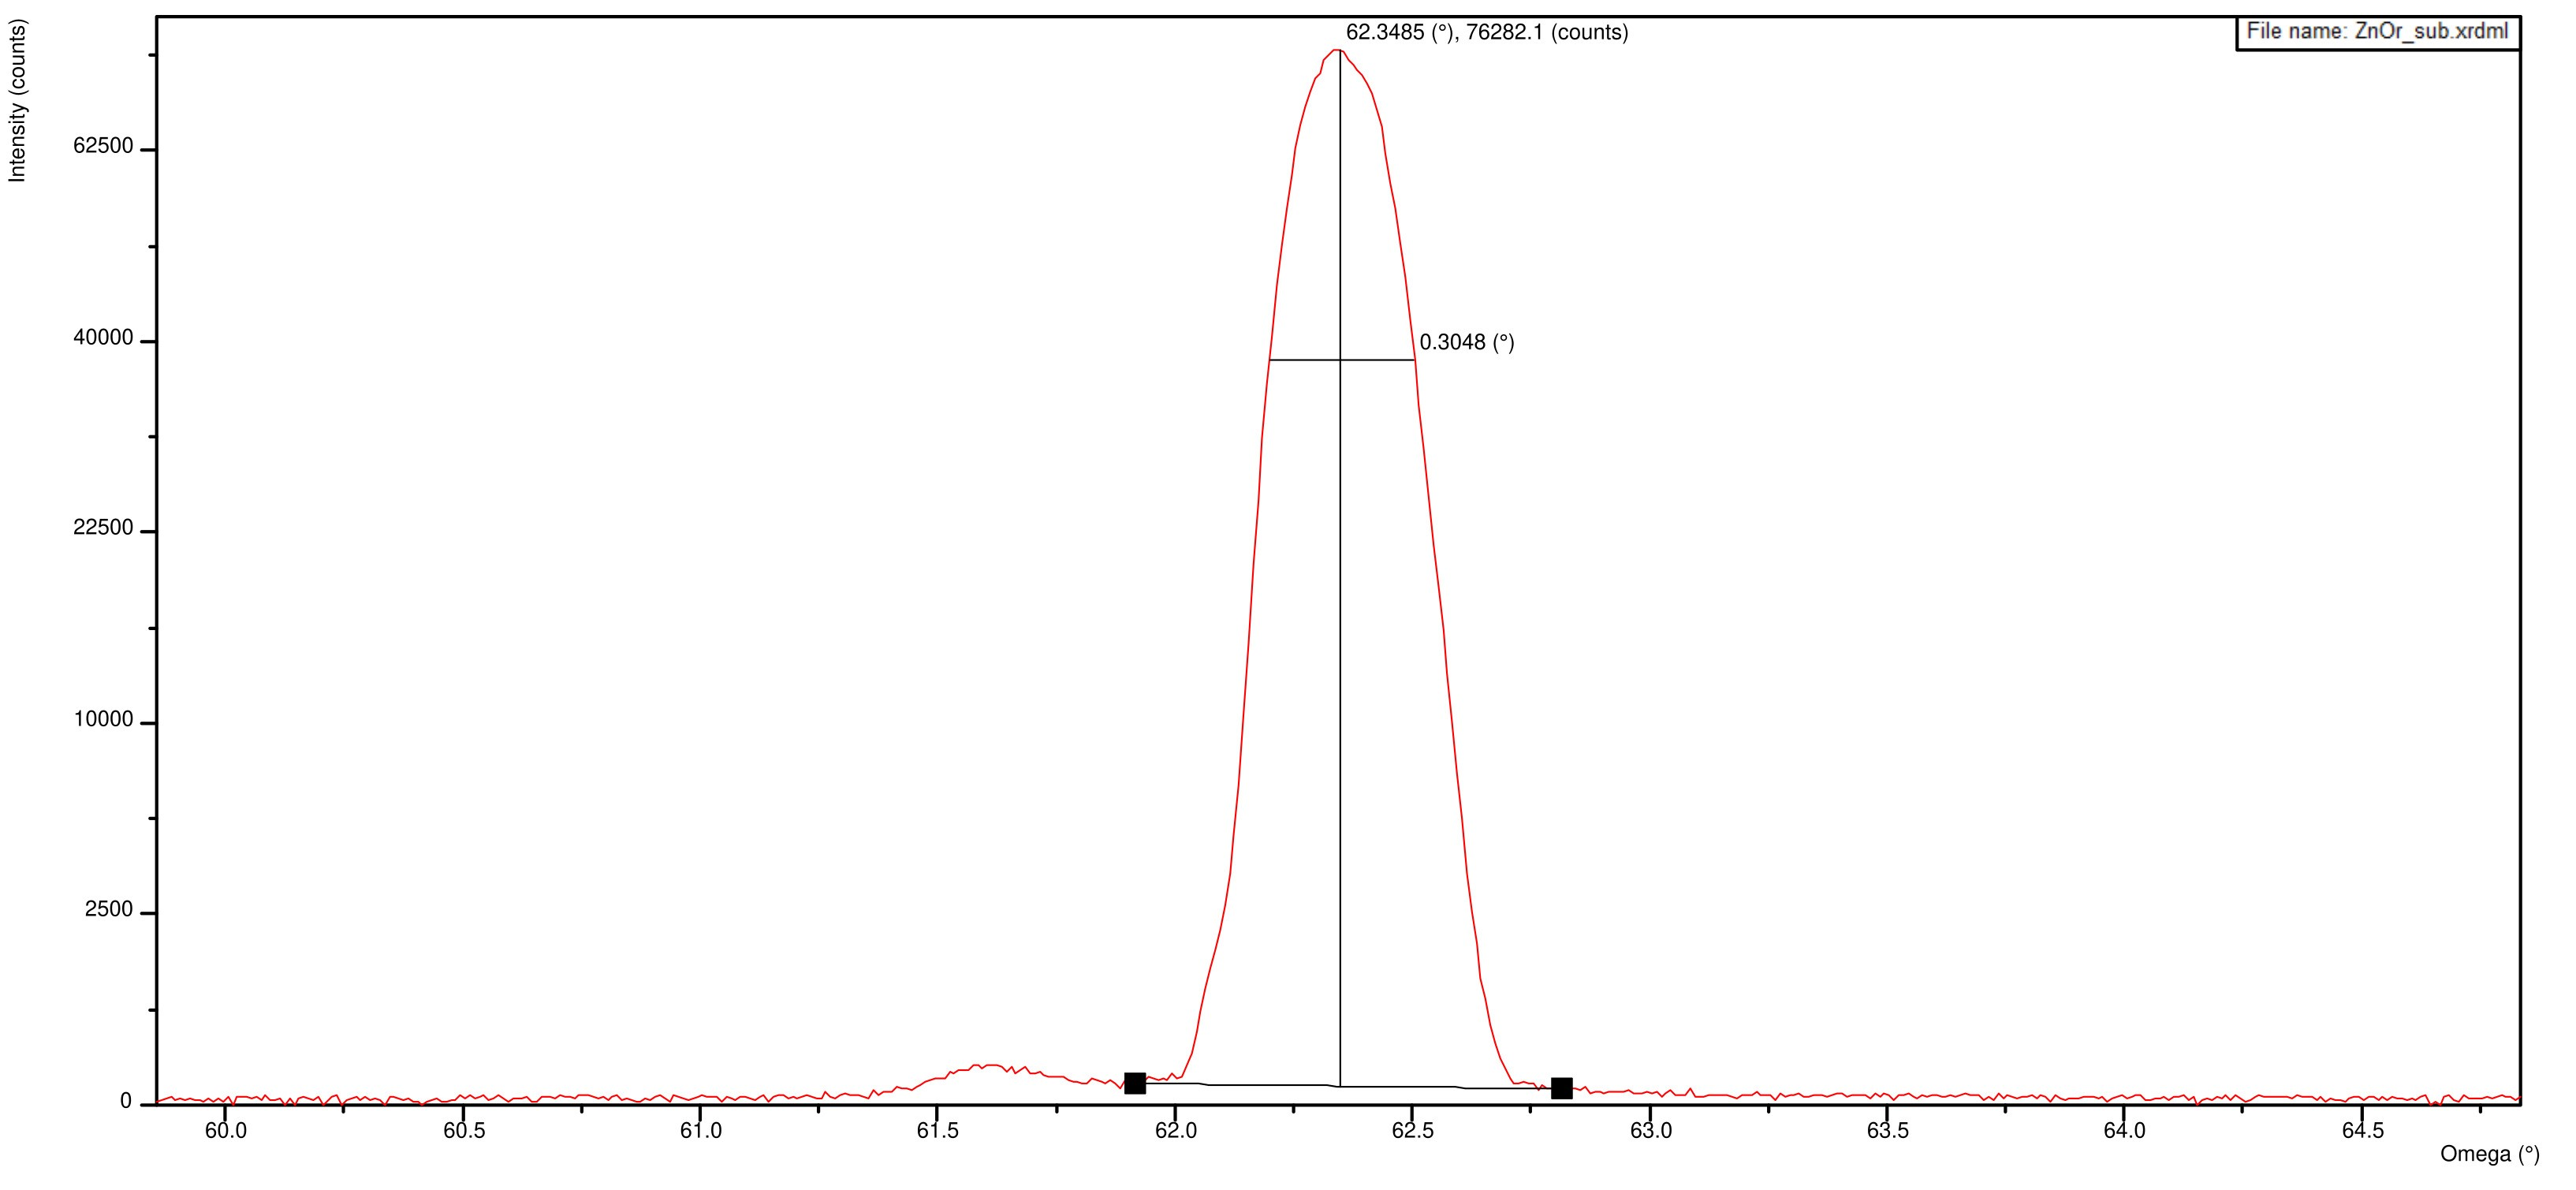
\includegraphics[width=\textwidth]{Figures/w-scan-r-plane-sapphire-peaks.jpg} % Replace with your image file
        \caption{r-plane ZnO peak}
        \label{fig:subfig3}
    \end{subfigure}
    \hfill
    \begin{subfigure}[b]{0.45\textwidth}
        \centering
        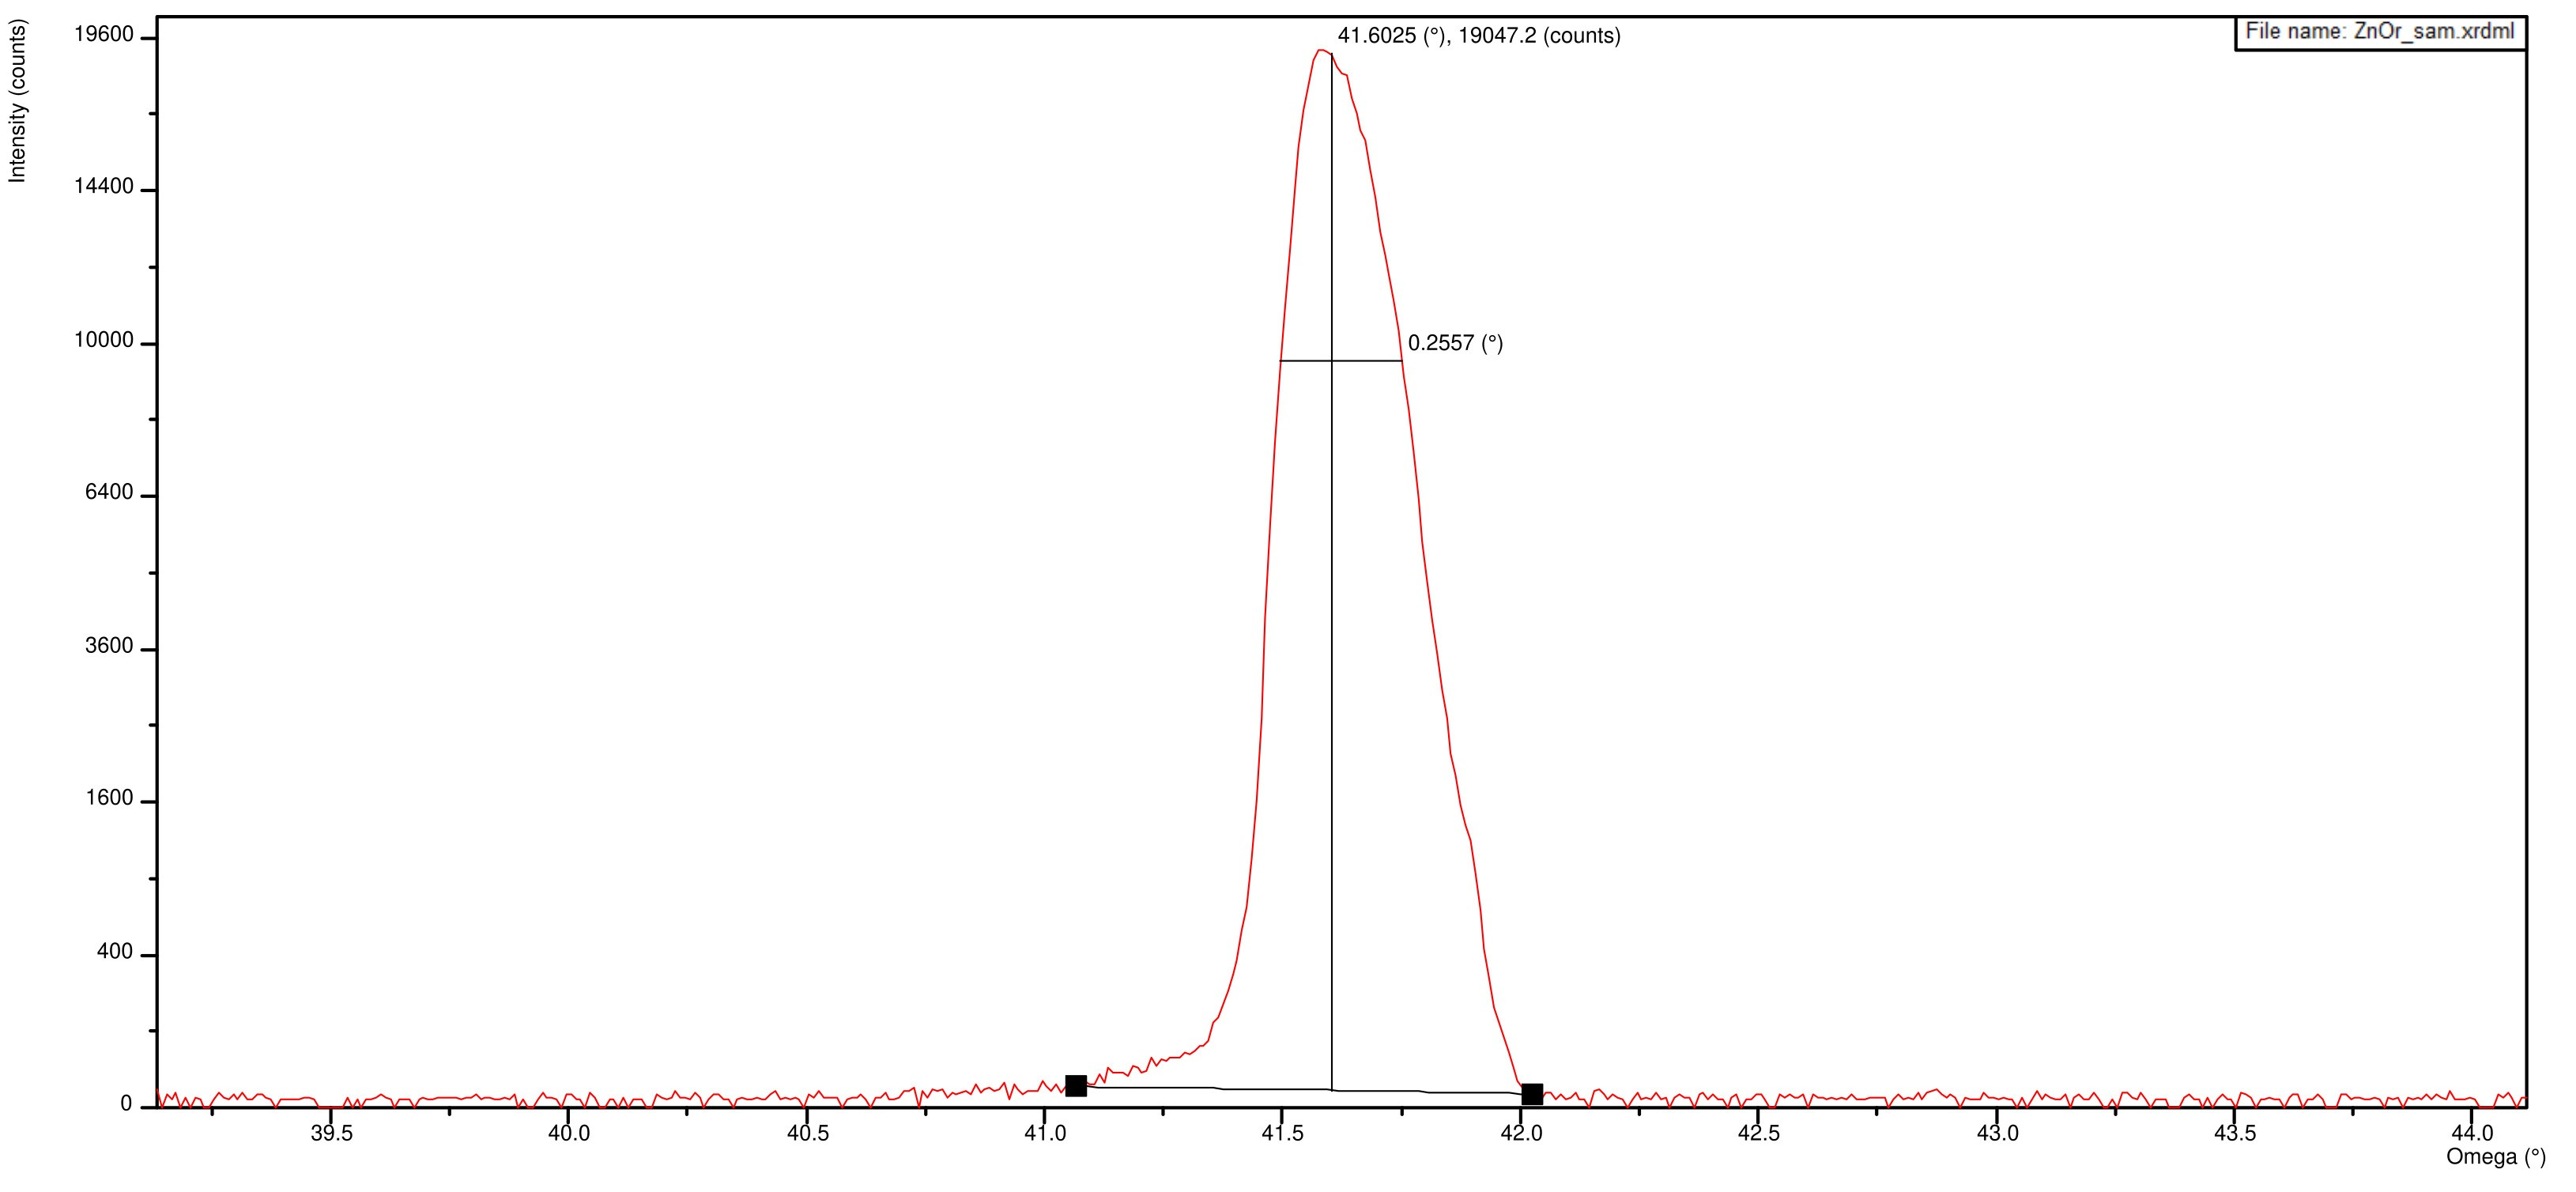
\includegraphics[width=\textwidth]{Figures/w-scan-ZnO-on-r-plane-sapphire-peaks.jpg} % Replace with your image file
        \caption{r-plane sapphire peak}
        \label{fig:subfig4}
    \end{subfigure}

    \caption{$\omega$ scans with FWHM values}
    \label{fig:grouped}
\end{figure}

The FWHMs of ZnO and sapphire peaks are shown with their respective positions  in Table 5, for the a-plane and r-plane orientations. We include the $2\theta - \omega$ for comparison. 

\begin{table}[h]
    \centering
	\begin{tabular}{|ccc|c|c|}
	\hline
	\multicolumn{3}{|c|}{}                                                             & $2 \theta - \omega$ & $\omega$   \\ \hline
	\multicolumn{1}{|c|}{\multirow{4}{*}{a plane}} & \multicolumn{1}{c|}{\multirow{2}{*}{Sapphire}} & Position & 80.671  & 40.4392 \\ \cline{3-5} 
	\multicolumn{1}{|c|}{} & \multicolumn{1}{c|}{}                          & FWHM     & 0.11          & 0.2317  \\ \cline{2-5} 
	\multicolumn{1}{|c|}{} & \multicolumn{1}{c|}{\multirow{2}{*}{ZnO}} & Position & 72.5915       & 62.8663 \\ \cline{3-5} 
	\multicolumn{1}{|c|}{} & \multicolumn{1}{c|}{}                          & FWHM     & 0.183         & 0.4042  \\ \hline
	\multicolumn{1}{|c|}{\multirow{4}{*}{r plane}} & \multicolumn{1}{c|}{\multirow{2}{*}{Sapphire}} & Position & 56.5733 & 41.6025 \\ \cline{3-5} 
	\multicolumn{1}{|c|}{} & \multicolumn{1}{c|}{}                          & FWHM     & 0.197         & 0.2557  \\ \cline{2-5} 
	\multicolumn{1}{|c|}{} & \multicolumn{1}{c|}{\multirow{2}{*}{ZnO}} & Position & 52.575        & 62.3485 \\ \cline{3-5} 
	\multicolumn{1}{|c|}{} & \multicolumn{1}{c|}{}                          & FWHM     & 0.098         & 0.3048  \\ \hline
	\end{tabular}
\end{table}



We see that the FWHMs obtained from the $2\theta - \omega$ scans are smaller than those obtained from the $\omega$ scans. This means that crystal mosaicity (in our case, tilt mosaicity) significantly affects the FWHM values. We also observe smaller FWHMs of the substrate in comparison with the sample (except for the r-plane $\omega$ scan, which is probably due to a technical error), which is because sapphire has a better order than the sample (since the sample was grown on top of it).


	The lattice parameters are calculated and shown in Table 6: 

\begin{table}[h]
\centering
\begin{tabular}{|c|c|c|}
\hline
ZnO                      & a      & c      \\ \hline
Task 1                   & 3.2493 & 5.2001 \\ \hline
Task 2                   & 3.2494 & 5.2070 \\ \hline
Theoretical PC-PDF value & 3.2499 & 5.2066 \\ \hline
\end{tabular}
\end{table}

\pagebreak{}

\subsection{Task 3}


In this task, we analyze an unknown sample (Powder No. 4) and use X'Pert Highscore to find 3 candidates and decide which one is the most likely. 

\begin{figure}[h]
	\centering
	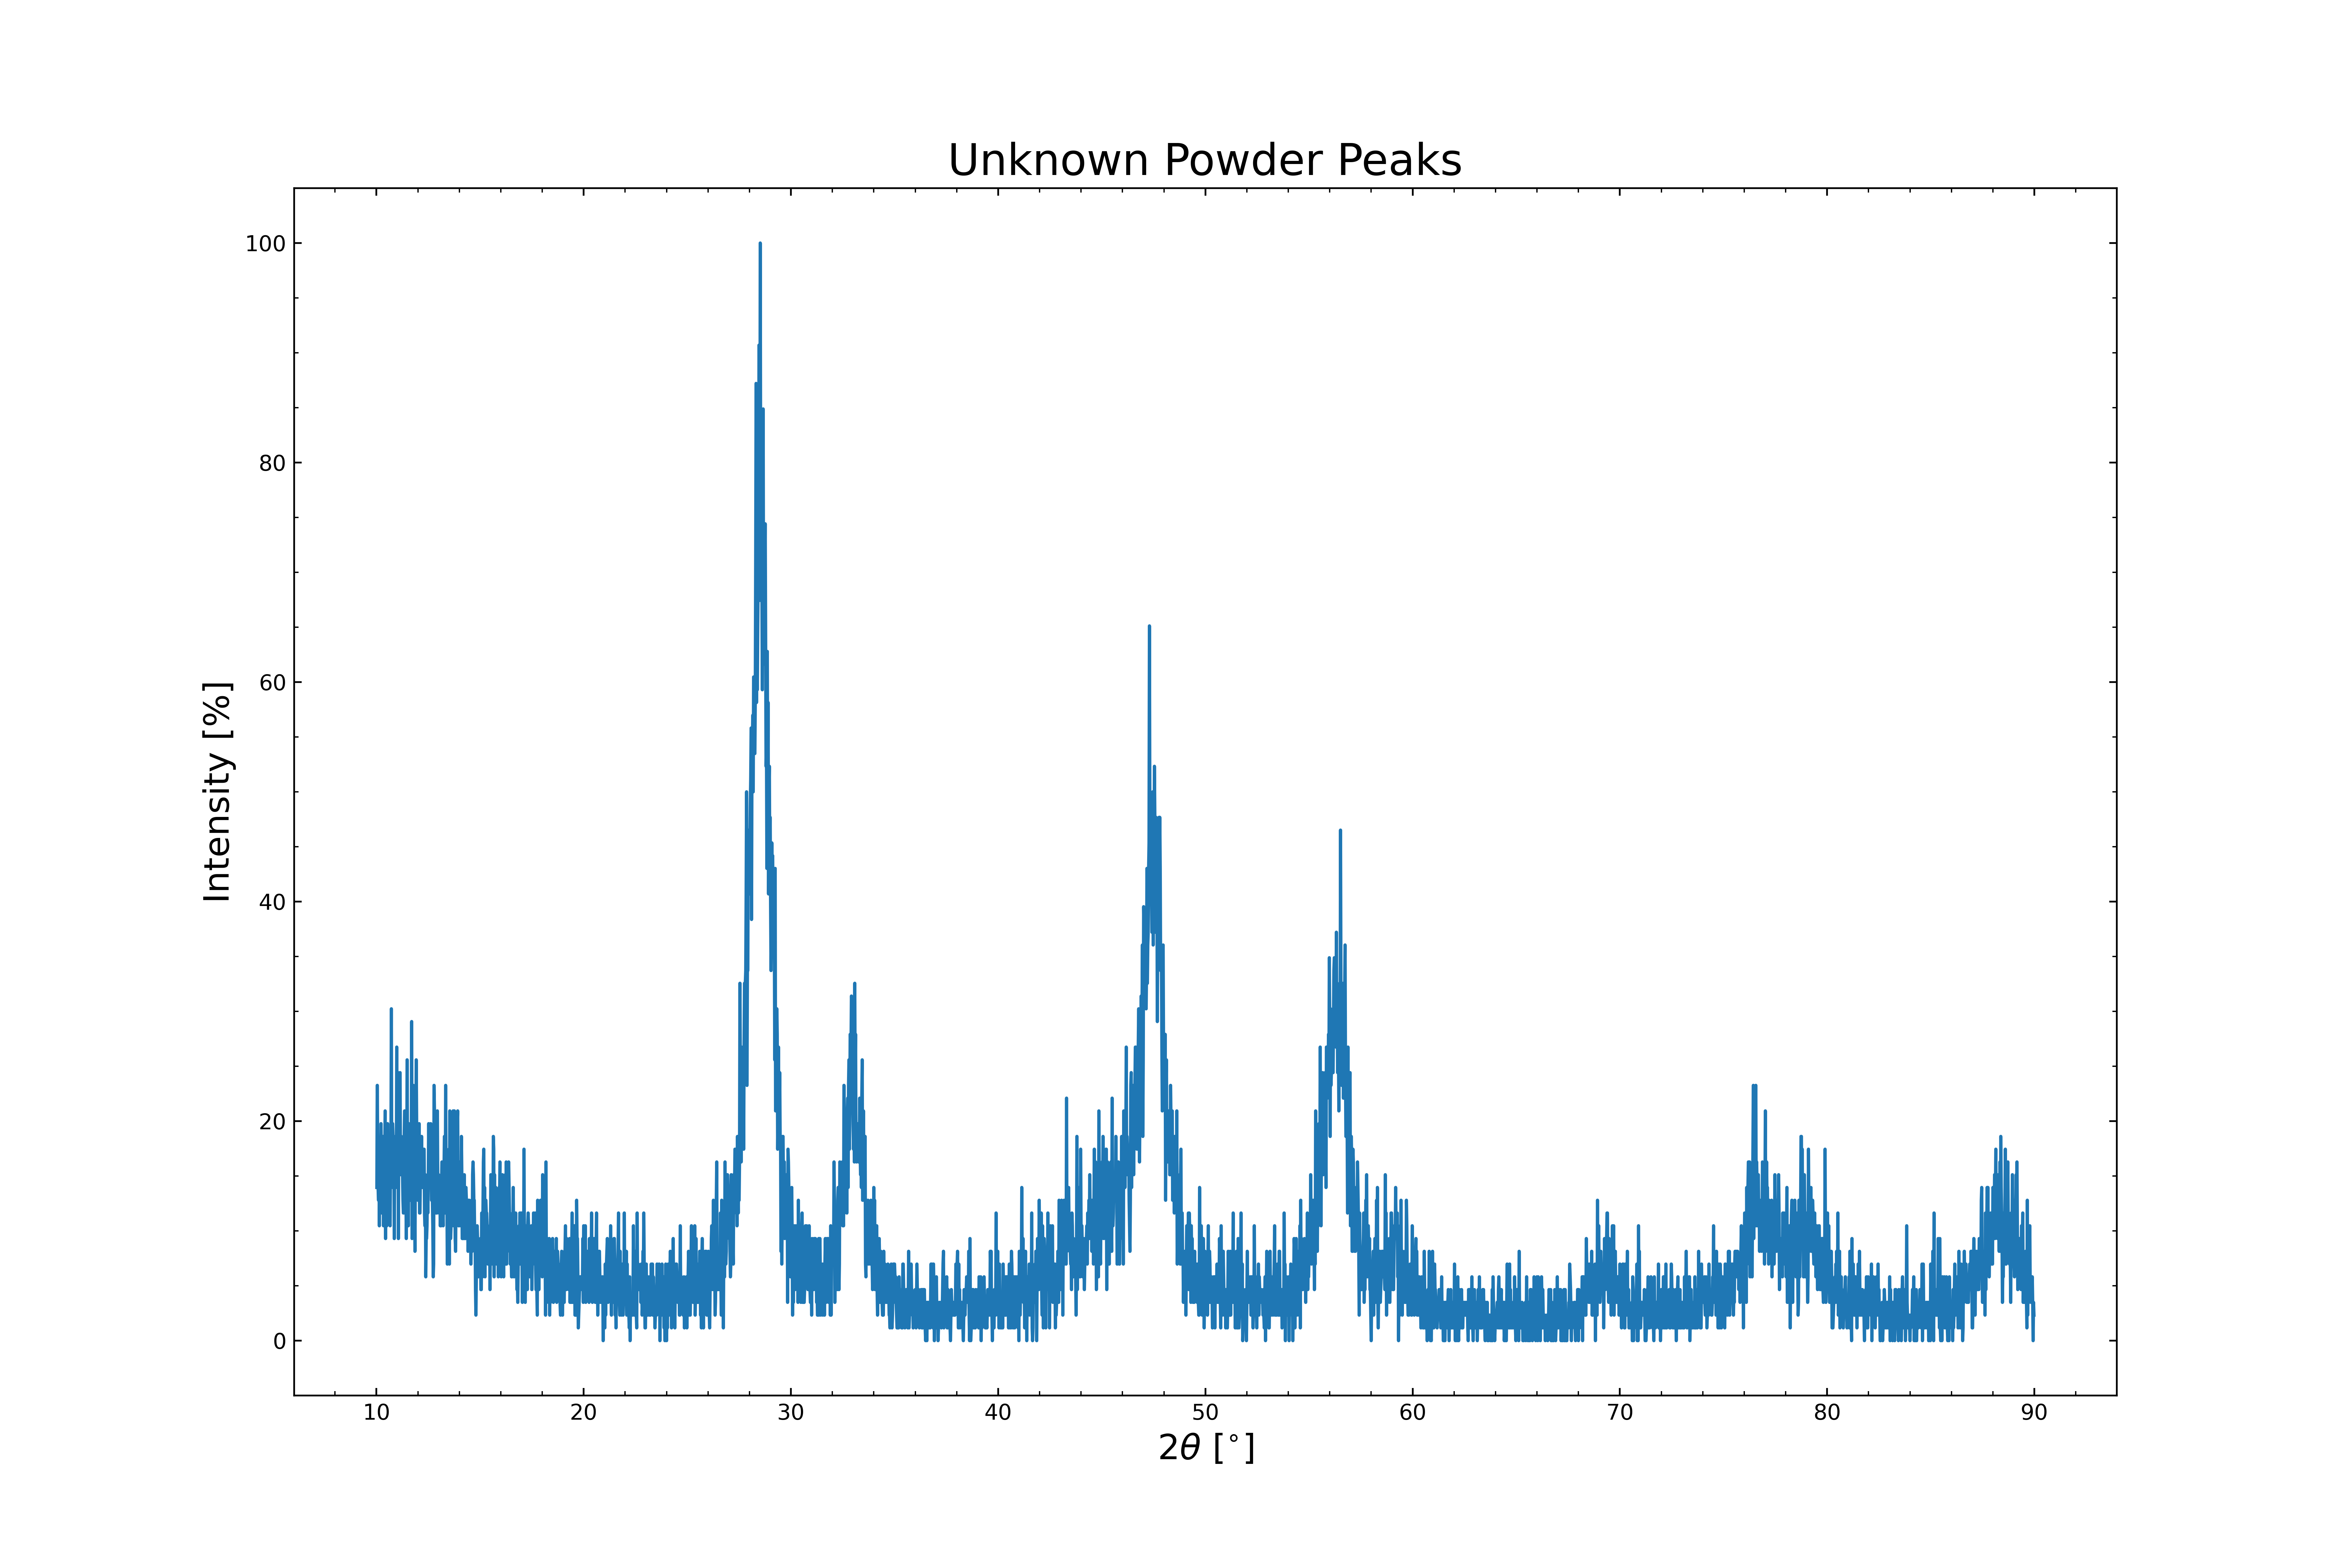
\includegraphics[width=\textwidth]{Figures/UnknownPowderPeaks.png}
	\caption{Bragg peaks of the unknown sample.}
	\label{fig:UnknownPeaks}
\end{figure}

Although this was a $2\theta - \omega$ scan done on a powder sample, the graph was noticably noisier than the ones in Task 1 (Figure [\ref{fig:BraggPeaks}]). This is probably human error; as part of the task was to manually squeeze the powder, which might not have been done properly.


	Furthermore, there are less peaks in general, which could be attributed to noise, but also to the fact that the scan was only done for $0^{\circ} \leq 2\theta \leq 90^{\circ}$
Still, the peaks compared using the $ 2 \theta $ values of the peaks from the PC-PDF database, and X'Pert Highscore found 5 possible candidates:

\begin{figure}[h]
	\centering
	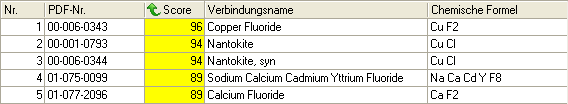
\includegraphics[width=\textwidth]{Figures/UnknownPowder.PNG}
	\caption{Table of PC-PDF database results for the unknown sample.}
	\label{fig:UnknownPowder}
\end{figure}

Of these 5, Copper Fluoride, Nantokite, and Calcium Fluoride were chosen as the 3 candidates. Nantokite, syn is the same as nantokite (just synthetic) so it was ignored. Sodium Calcium Cadmium Yttrium Fluoride had the same score as Calcium Fluoride, so Calcium Fluoride was chosen purely because it seemed like the more simple (and hence more likely for the lab to have) compound. Their peaks are shown in [\ref{appendix:PCPDFPeaks}] 

\pagebreak{}

	This is what each powder looks like:

\begin{figure}[h]
	\centering
	\begin{subfigure}{0.45\textwidth}
		\centering
		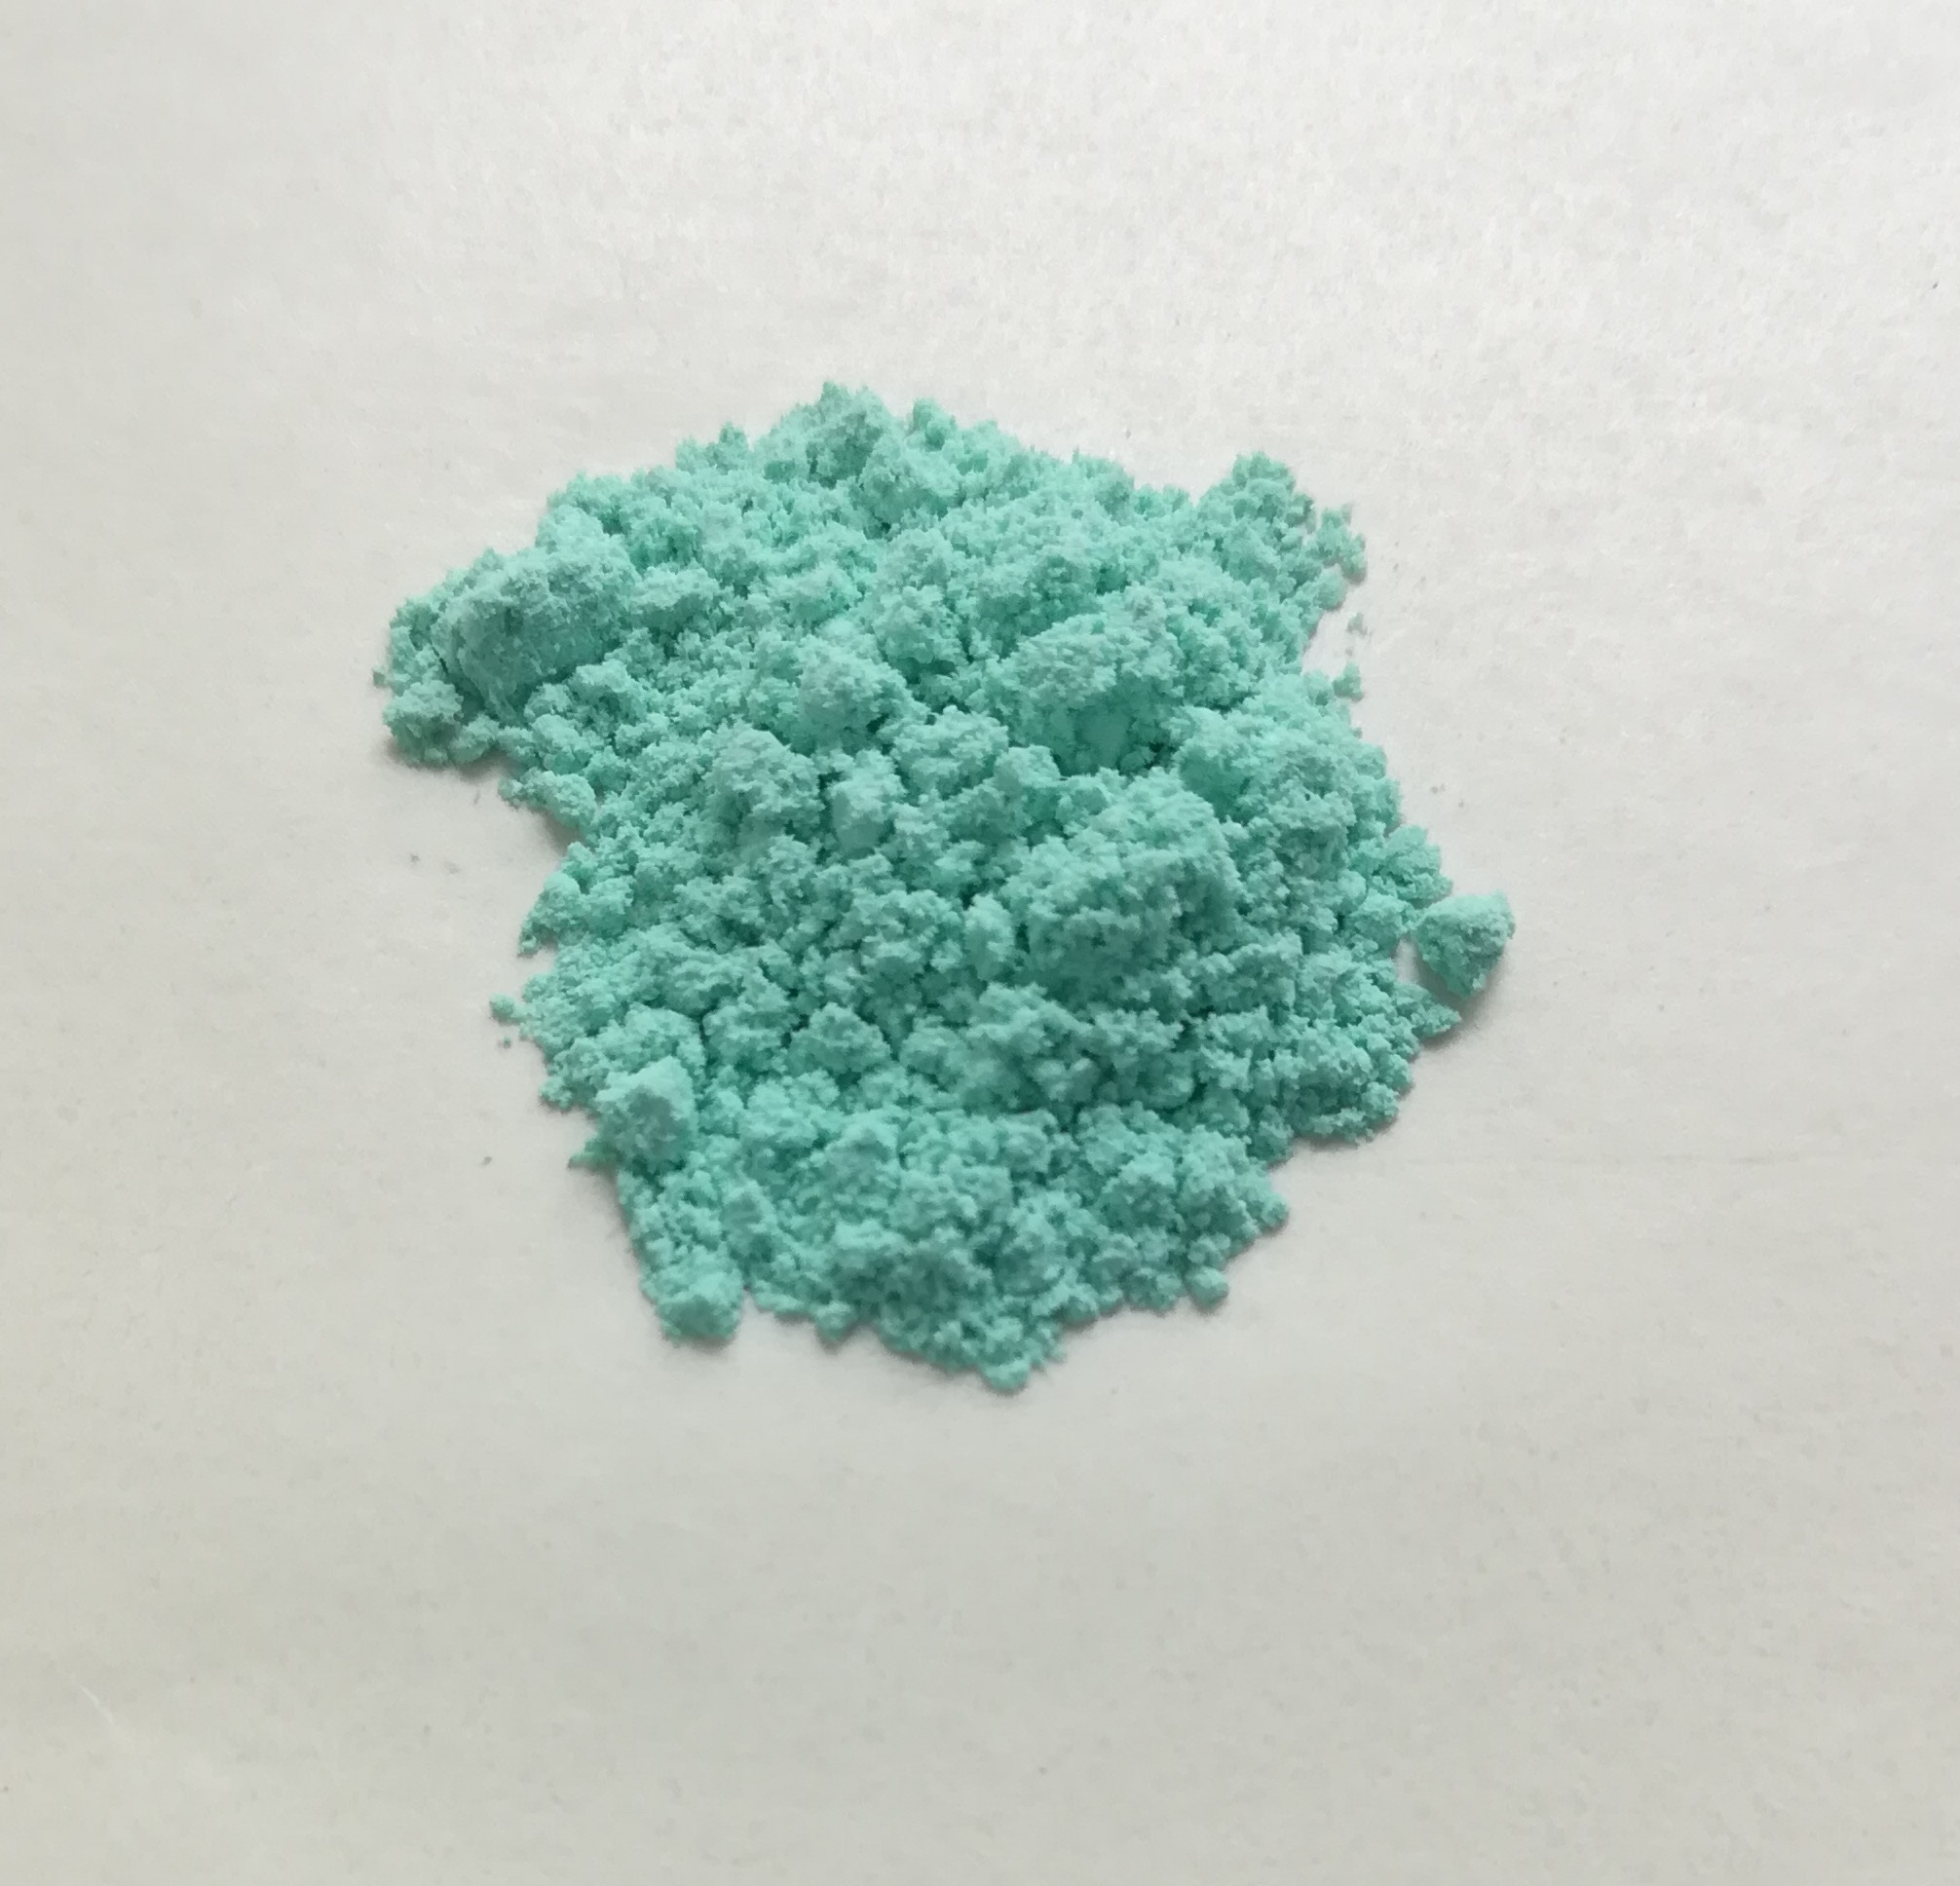
\includegraphics[width=\textwidth]{Figures/CuF2.jpg}
		\caption{Copper (II) Fluoride. \cite{leiem_2019_copperii} }
		\label{fig:CuF2}
	\end{subfigure}
	\hfill
	\begin{subfigure}{0.45\textwidth}
		\centering
		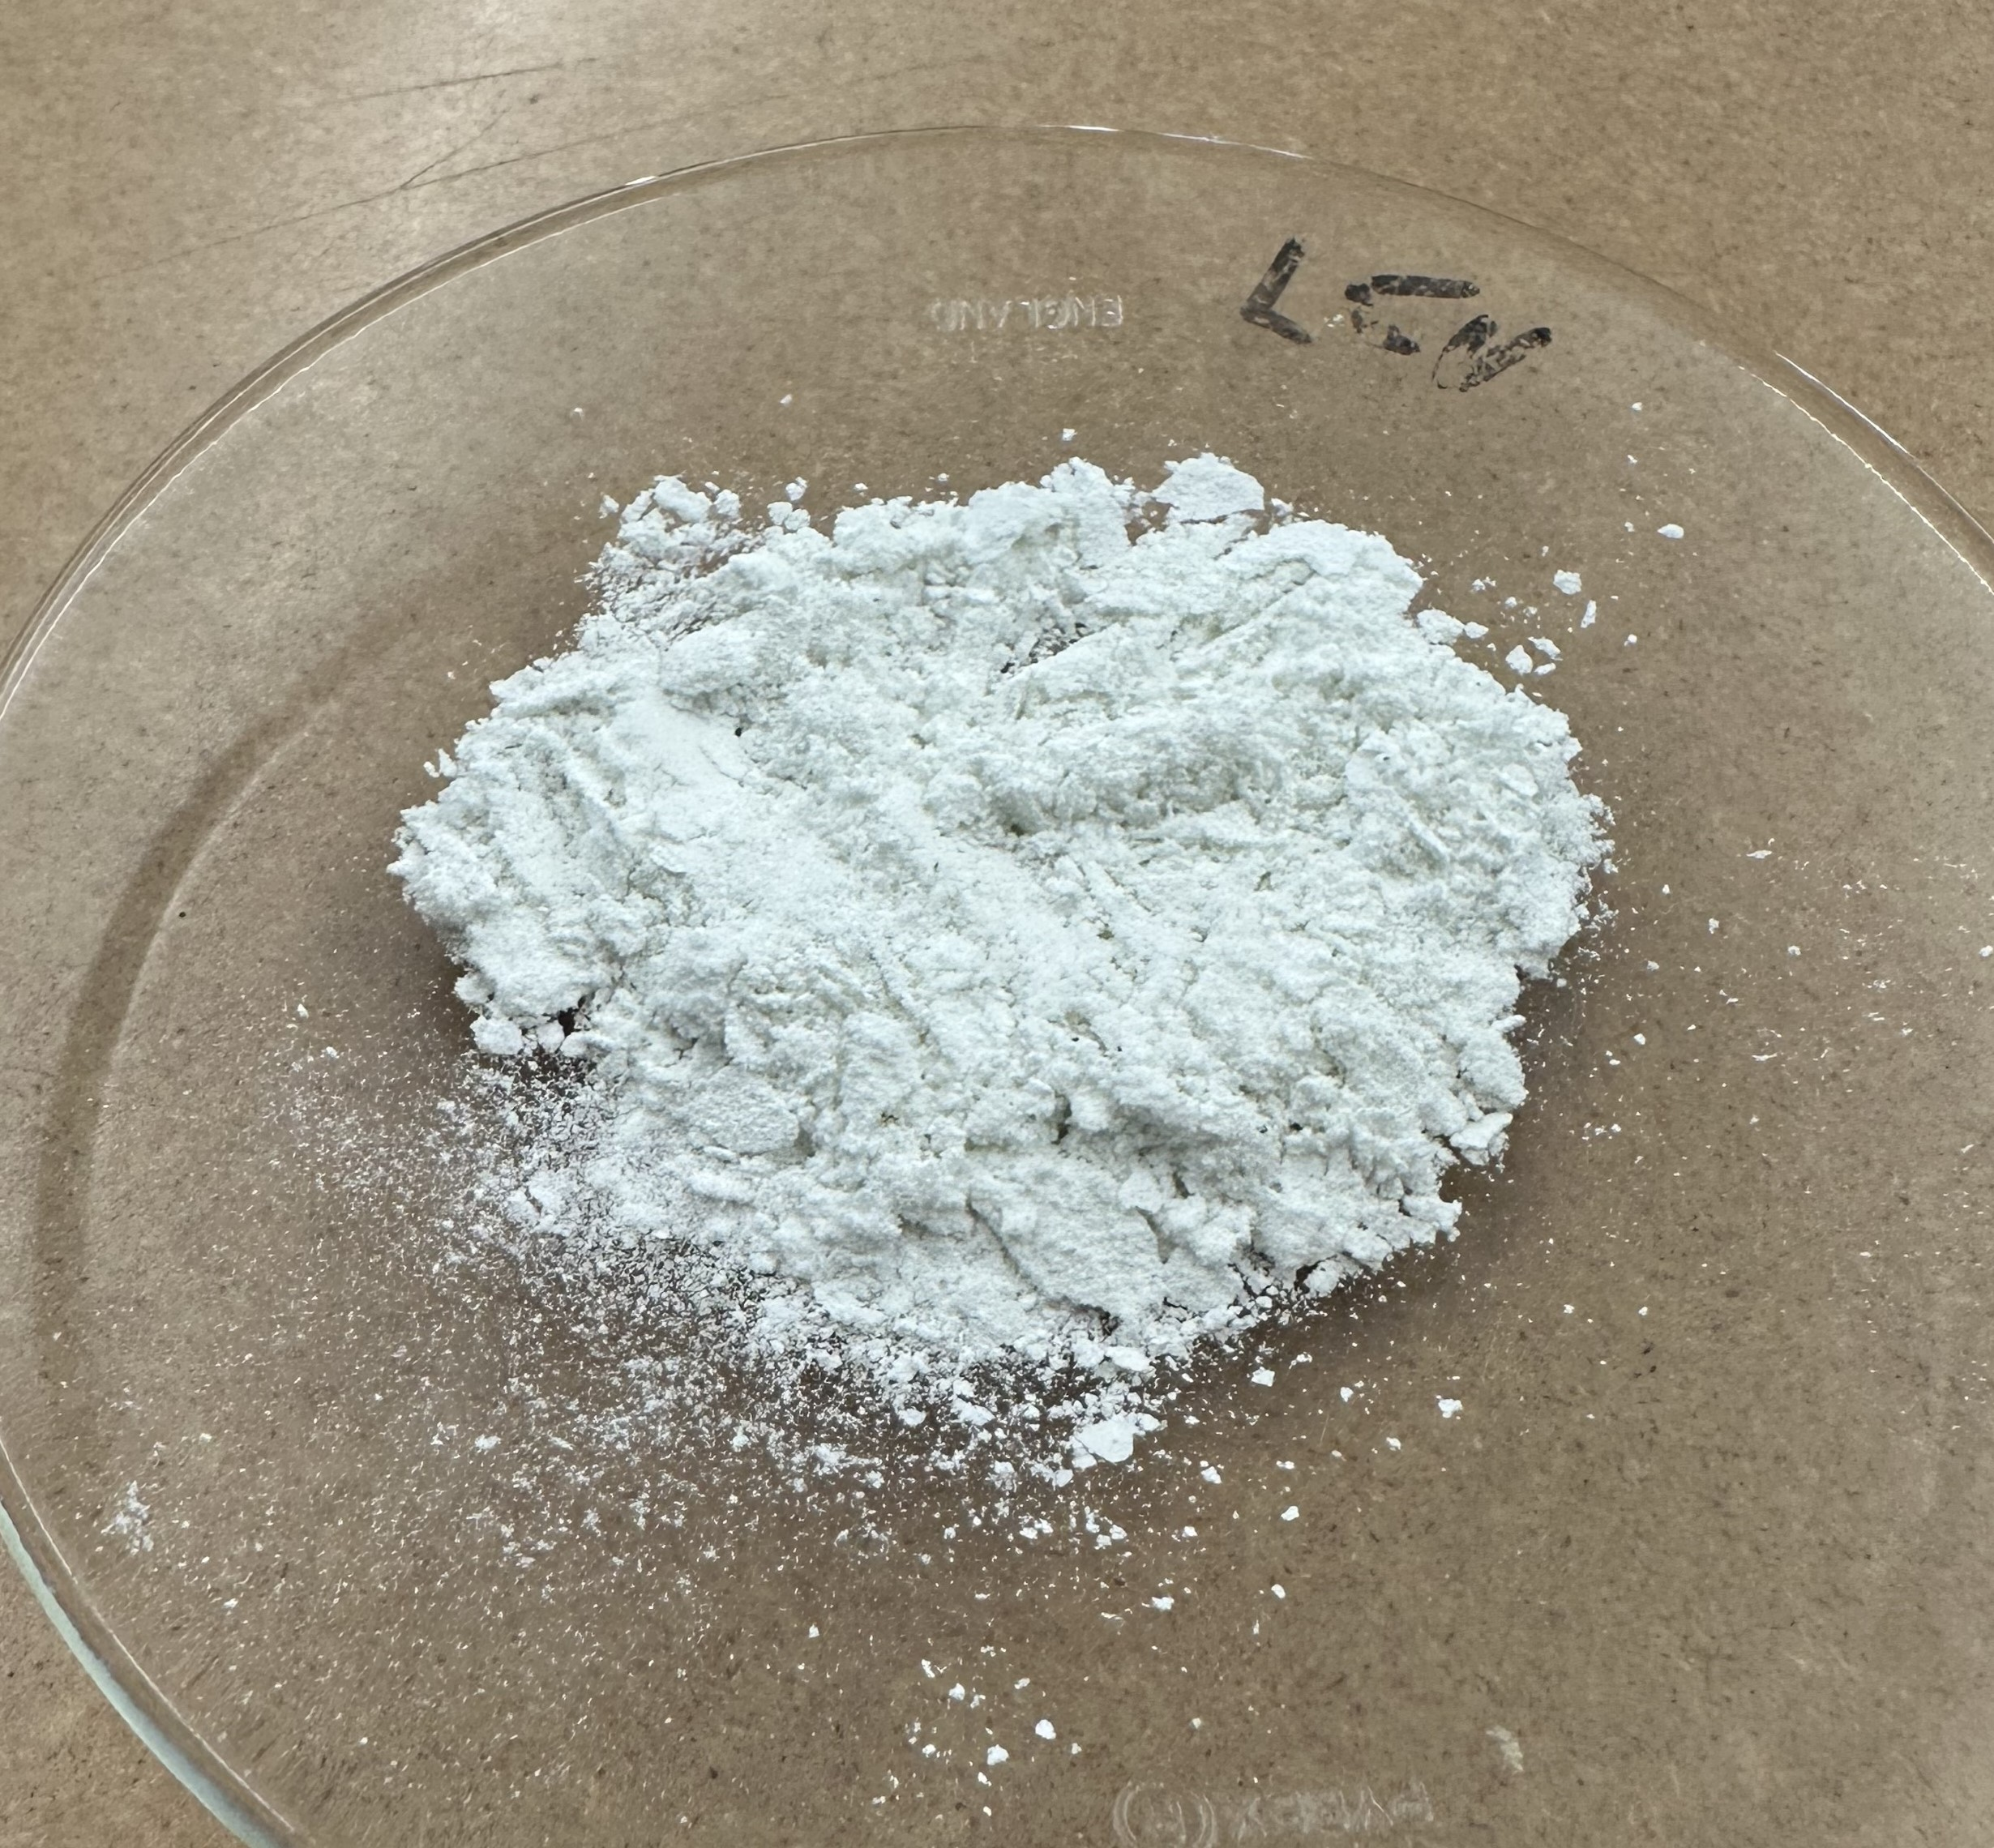
\includegraphics[width=\textwidth]{Figures/CuCl.jpg}
		\caption{Nantokite ( Copper (I) Chloride). \cite{keresluna_2023_copper}}
		\label{fig:Nantokite}
	\end{subfigure}
	\vfill
	\begin{subfigure}{0.45\textwidth}
		\centering
		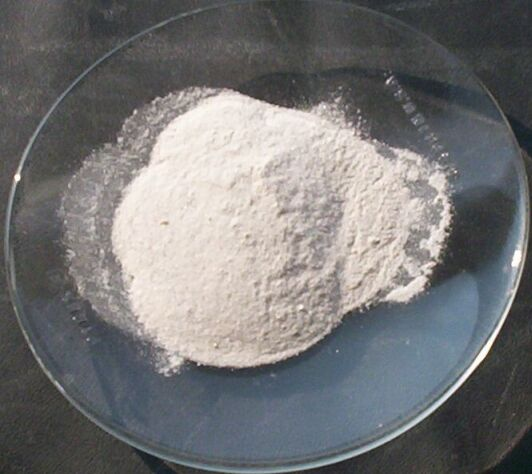
\includegraphics[width=\textwidth]{Figures/CaF2.jpg}
		\caption{Calcium Fluoride. \cite{june2005_2005_calcium}}
		\label{fig:CaF2}
	\end{subfigure}
	\label{fig:UnknownPowders}
\end{figure}

This immediately discounts Copper (II) Fluoride, as the powder that we dealed with was white in color, leaving Nantokite and Calcium Fluoride as the remaining candidates.


Nantokite had the higher score, so it reasonable to choose it as the most likely candidate. However, It could very well be Calcium Fluoride. This method of trying to know the chemical formula of an unknown compound 
is not very accurate, due to the large noise present in the data and the low range of $2\theta$ values. Both of these factors make it hard to accurately match the peaks of the unknown sample with the PC-PDF database. 


	Furthermore, looking closely at the peaks in [\ref{appendix:PCPDFPeaks}], Figure [\ref{fig:UnknownPeaks}] seems to match the Nantokite peaks more than the CaF2 peaks; since the CaF2 pattern has a 3rd peak with 100\% intensity at $2\theta \approx 47^{\circ}$, and in Figure [\ref{fig:UnknownPeaks}] the peak there is not at 100 \%. So, our sample is most likely Nantokite. Still, further analysis is needed to be certain. 
\pagebreak{}

\section{Conclusion}

In Task 1, we analyzed the diffraction patterns of two polycrystalline bulk samples, Silicon (Si) and Zinc Oxide (ZnO). By performing peak indexing and error analysis, we estimated the lattice parameters with relative errors of 0.04\% for Silicon and 0.02\% and 0.1\% for the \(a\) and \(c\) parameters of ZnO, respectively.

In Task 2, an epitaxied thin film ZnO sample was analyzed. The peaks observed for the isotropic powder sample mostly vanished in this case for both of the substrate orientations (r-plane and a-plane). Next, we carried out$\omega$ scans of the two samples for the peaks with the highest $2\theta$ values, which revealed the degree of misalignment in the two samples. We only observe a minor change for the lattice parameters values in comparison with the calculation from the powder sample.

Finally, in Task 3, we identified a structural similarity between an unknown powder sample and Nantokite. This task highlighted the significance of XRD in determining crystal structures, although it does not provide information about chemical composition.

\pagebreak{}

\begin{appendices}

\section{Equations \cite{bernarddeniscullity_2015_elements}} 
\label{appendix:Equations}
Cubic Unit Cell:

\begin{gather*}
	\label{eq:cubic}
	a = b =c, \ \alpha = \beta = \gamma = 90^{\circ} \\
	\frac{1}{d^2} = \frac{h^2 + k^2 + l^2}{a^2}
\end{gather*}

Tetragonal Unit Cell:

\begin{gather*}
	\label{eq:tetragonal}
	a = b \neq c, \ \alpha = \beta = \gamma = 90^{\circ} \\
	\frac{1}{d^2} = \frac{h^2 + k^2}{a^2} + \frac{l^2}{c^2}
\end{gather*}

Hexagonal Unit Cell:
\begin{gather*}
	\label{eq:hexagonal}
	a = b \neq c, \ \alpha = \beta = 90^{\circ}, \ \gamma = 120^{\circ} \\
	\frac{1}{d^2} = \frac{4}{3}\left(\frac{h^2 + hk + k^2}{a^2}\right) + \frac{l^2}{c^2}
\end{gather*}

Rhombohedral Unit Cell:

\begin{gather*}
	\label{eq:rhombohedral}
	a = b = c, \ \alpha = \beta = \gamma \neq 90^{\circ} \\
	\frac{1}{d^2} = \frac{(h^2 + k^2 + l^2)\sin^2 \alpha + 2(hk + hl + kl)\cos^2 \alpha - \cos \alpha}{a^2(1-3\cos^2 \alpha + 2\cos^3 \alpha)}
\end{gather*}

Orthorhombic Unit Cell:

\begin{gather*}
	\label{eq:orthorhombic}
	a \neq b \neq c, \ \alpha = \beta = \gamma = 90^{\circ} \\
	\frac{1}{d^2} = \frac{h^2}{a^2} + \frac{k^2}{b^2} + \frac{l^2}{c^2}
\end{gather*}

Monoclinic Unit Cell:

\begin{gather*}
	\label{eq:monoclinic}
	a \neq b \neq c, \ \alpha = \gamma = 90^{\circ}, \ \beta \neq 90^{\circ} \\
	\frac{1}{d^2} = \frac{1}{\sin^2(\beta)}\left(\frac{h^2}{a^2} + \frac{k^2 \sin^2\beta}{b^2}+ \frac{l^2}{c^2} - 2\frac{hl \cos \beta}{ac}\right)
\end{gather*}

Triclinic Unit Cell:

\begin{gather*}
	\label{eq:triclinic}
	a \neq b \neq c, \ \alpha \neq \beta \neq \gamma \neq 90^{\circ} \\
	\frac{1}{d^2} = \frac{1}{V^2}\left(S_{11} h^2 + S_{22} k^2 + S_{33} l^2 + 2(S_{12} hk +S_{23} kl + S_{13} hl)  \right) \\
	\begin{align*}
	\text{where} \\
	S_{11} &= b^2c^2 \sin^2 \alpha \\
	S_{22} &= a^2c^2 \sin^2 \beta \\
	S_{33} &= a^2b^2 \sin^2 \gamma \\
	S_{12} &= abc^2(\cos \alpha \cos \beta - \cos \gamma) \\
	S_{23} &= a^2bc(\cos \beta \cos \gamma - \cos \alpha) \\
	S_{13} &= ab^2c(\cos \alpha \cos \gamma - \cos \beta) \\
	V &= abc\sqrt{1 - \cos^2 \alpha - \cos^2 \beta - \cos^2 \gamma + 2\cos \alpha \cos \beta \cos \gamma}
	\end{align*}
\end{gather*}

\pagebreak{}

\section{PC-PDF Peaks}
\label{appendix:PCPDFPeaks}
\begin{figure*}[h]
	\centering
	\begin{subfigure}{0.45\textwidth}
		\centering
		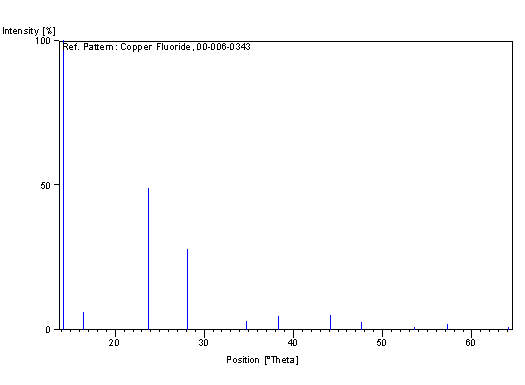
\includegraphics[width=\textwidth]{Figures/CuF2Peaks.png}
		\caption{Copper Fluoride.}
		\label{fig:CuF2Peaks}
	\end{subfigure}
	\hfill
	\begin{subfigure}{0.45\textwidth}
		\centering
		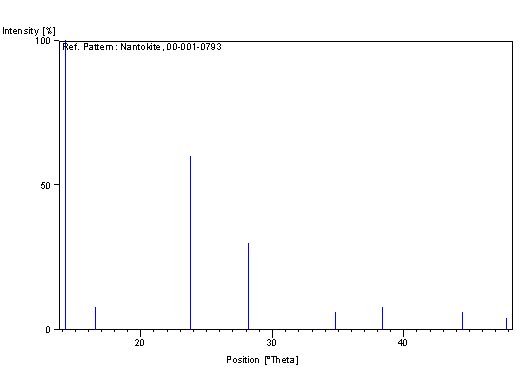
\includegraphics[width=\textwidth]{Figures/NantokitePeaks.png}
		\caption{Nantokite.}
		\label{fig:NantokitePeaks}
	\end{subfigure}
	\begin{subfigure}{0.45\textwidth}
		\centering
		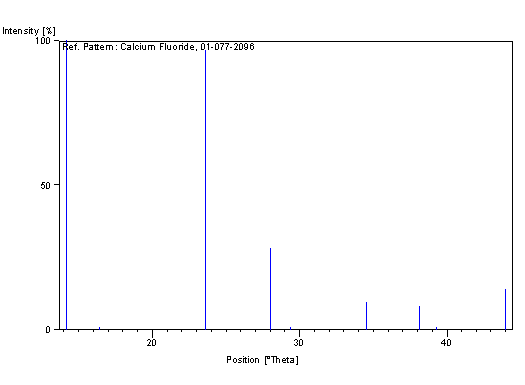
\includegraphics[width=\textwidth]{Figures/CaF2Peaks.png}
		\caption{Calcium Fluoride.}
		\label{fig:CaF2Peaks}
	\end{subfigure}
	\label{fig:PCPDFPeaks}
\end{figure*}

\end{appendices}

\pagebreak{}

\bibliographystyle{ieeetr} 
\bibliography{XRD} 

\end{document}